%%%%%%%%%%%%%%%%%%%%%%%%%%%%%%%%%%%%%%%%%%%%%%%%%%%%%%%%%%%%%%%%%%%%%%%%%%%%%%%%%%%%%
\section{Introduction}\label{sec:mtd_intro}
%%%%%%%%%%%%%%%%%%%%%%%%%%%%%%%%%%%%%%%%%%%%%%%%%%%%%%%%%%%%%%%%%%%%%%%%%%%%%%%%%%%%%

HAWC's current software suite, plugins to 3ML and HAL \cite{2021arXiv211201818M,Abeysekara_2017}, do not fully utilize computational advancements of recent decades.
Said advancements include the proliferation of Graphical Processing Units (GPUs), and multithreading on multicore processors.
The analysis described in \Cref{sec:glory_duck} took up to 3 months of wall time waiting for the full gambit of data analysis and simulation of background to compute.
Additionally, with the updated 2D energy binning scheme split by $f_\mathrm{hit}$ and estimated energy from our Neural Network (NN) method, the time needed to compute was expected to grow.
Although excessive computing time was, in part, from an intense use of a shared computing cluster, it was evident that there was room for improvement.
In HAWC's next generation dSph DM search, I decided to develop codes that would utilize the multicore processors on modern high performance computing clusters.
The results of this work are featured in this chapter and brought a human timing improvement to computation that scales approximately as $1/N$ where $N$ is the number of threads.

%%%%%%%%%%%%%%%%%%%%%%%%%%%%%%%%%%%%%%%%%%%%%%%%%%%%%%%%%%%%%%%%%%%%%%%%%%%%%%%%%%%%%
\section{Dataset and Background}\label{sec:mtd_databgd}
%%%%%%%%%%%%%%%%%%%%%%%%%%%%%%%%%%%%%%%%%%%%%%%%%%%%%%%%%%%%%%%%%%%%%%%%%%%%%%%%%%%%%

This section describes the data and background methods used for HAWC's multithreaded study of dSphs.
\Cref{sec:mtd_data,sec:mtd_tools} are most useful for fellow HAWC collaborators looking to replicate a multithreaded dSph DM search.

%%%%%%%%%%%%%%%%%%%%%%%%%%%%%%%%%%%%%%%%%%%%%%%
\subsection{Itemized HAWC files}\label{sec:mtd_data}
%%%%%%%%%%%%%%%%%%%%%%%%%%%%%%%%%%%%%%%%%%%%%%%
These files are only available within HAWC's internal documentation and collaborators.
They are not meant for public access, and are presented here so that HAWC can reproduce results accurately.

\begin{itemize}
    \item Detector Resolution: \texttt{refit-Pass5-Final-NN-detRes-zenith-dependent.root}
    \item Data Map: \texttt{Pass5-Final-NN-maptree-ch103-ch1349-zenith-dependent.root}
    \item Spectral Dictionary: \texttt{HDMSpectra\_dict\_gamma.npy}
\end{itemize}

% %%%%%%%%%%%%%%%%%%%%%%%%%%%%%%%%%%%%%%%%%%%%%%%
\subsection{Software Tools and Development}\label{sec:mtd_tools}
%%%%%%%%%%%%%%%%%%%%%%%%%%%%%%%%%%%%%%%%%%%%%%%

This analysis was performed using HAL and 3ML \cite{Abeysekara_2017, vianello2015multimission} in Python3.
I built software in collaboration with Michael Martin and Letrell Harris to implement the \emph{Dark Matter Spectra from the Electroweak to the Planck Scale} (HDM) \cite{Rodd:HDM_spec} and dSphs spatial model from \cite{DM_Strigari20} for HAWC analysis.
A NumPy dictionary of HDM, \texttt{HDMSpectra\_dict\_gamma.npy}, was made for portability within the collaboration.
These dictionaries were generated from the \href{https://github.com/nickrodd/HDMSpectra/tree/master}{git repository} \cite{Rodd:HDM_spec}.
The analysis was performed using the Neural Network energy estimator for Pass 5.F.
A description of this estimator was provided in \cref{sec:hawc_nn}. Its key, relevant improvements are an improved energy estimation and improved sensitivities at higher zenith angles.
All other software used for data analysis, DM profile generation, and job submission to SLURM are kept in my sandbox in the \href{https://gitlab.com/hawc-observatory/sandboxes/salaza82/dark_matter_hawc}{Dark Matter HAWC} project.
The above repository also incorporates the model inputs used previously in Glory Duck, described in \Cref{sec:glory_duck}, so Glory Duck remains compatible with modern software.

%%%%%%%%%%%%%%%%%%%%%%%%%%%%%%%%%%%%%%%%%%%%%%%
\subsection{Data Set and Background Description} \label{sec:mtd_data_bkgd}
%%%%%%%%%%%%%%%%%%%%%%%%%%%%%%%%%%%%%%%%%%%%%%%

The HAWC data maps used for this analysis contain 2565 days of data between runs 2104 and 7476.
They were generated from pass 5.F reconstruction.
The analysis is performed using the NN energy estimator with nominal bin list:

\begin{itemize}
    \item[] \texttt{B1C0Ea}, \texttt{B1C0Eb}, \texttt{B1C0Ec}, \texttt{B1C0Ed}, \texttt{B1C0Ee}, \texttt{B2C0Ea}, \texttt{B2C0Eb}, \texttt{B2C0Ec}, \texttt{B2C0Ed}, \texttt{B2C0Ee}, \texttt{B3C0Ea}, \texttt{B3C0Eb}, \texttt{B3C0Ec}, \texttt{B3C0Ed}, \texttt{B3C0Ee}, \texttt{B3C0Ef}, \texttt{B4C0Eb}, \texttt{B4C0Ec}, \texttt{B4C0Ed}, \texttt{B4C0Ee}, \texttt{B4C0Ef}, \texttt{B5C0Ec}, \texttt{B5C0Ed}, \texttt{B5C0Ee}, \texttt{B5C0Ef}, \texttt{B5C0Eg}, \texttt{B6C0Ed}, \texttt{B6C0Ee}, \texttt{B6C0Ef}, \texttt{B6C0Eg}, \texttt{B6C0Eh}, \texttt{B7C0Ee}, \texttt{B7C0Ef}, \texttt{B7C0Eg}, \texttt{B7C0Eh}, \texttt{B7C0Ei}, \texttt{B8C0Ee}, \texttt{B8C0Ef}, \texttt{B8C0Eg}, \texttt{B8C0Eh}, \texttt{B8C0Ei}, \texttt{B8C0Ej}, \texttt{B9C0Ef}, \texttt{B9C0Eg}, \texttt{B9C0Eh}, \texttt{B9C0Ei}, \texttt{B9C0Ej}, \texttt{B10C0Eg}, \texttt{B10C0Eh}, \texttt{B10C0Ei}, \texttt{B10C0Ej}, \texttt{B10C0Ek}, \texttt{B10C0El}
\end{itemize}
Bin 0 was excluded as it has substantial hadronic contamination and poor angular resolution.
This list was cut down depending on the declination of the source because the Point Spread Function (PSF) of these bins were too large, or the statistics were too low.

Background considerations and source selection was identical to \cref{sec:gs_data_bkgd}, and no additional arguments are provided here.
Many of the HAWC systematics explored in \cref{sec:hawc_systematic} also apply for this DM search and are not discussed here.

%%%%%%%%%%%%%%%%%%%%%%%%%%%%%%%%%%%%%%%%%%%%%%%%%%%%%%%%%%%%%%%%%%%%%%%%%%%%%%%%%%%%%
\section{Analysis}\label{sec:mtd_analysis}
%%%%%%%%%%%%%%%%%%%%%%%%%%%%%%%%%%%%%%%%%%%%%%%%%%%%%%%%%%%%%%%%%%%%%%%%%%%%%%%%%%%%%

The analysis and its systematics are almost identical to \cref{sec:gd_analysis}.
Importantly, the same \cref{eq:id_dm_flux,eq:jfactor} for estimating the gamma-ray flux at HAWC from our sources are used here.

This analysis improves on \Cref{sec:glory_duck} in the following ways.
The particle physics model used for gamma-ray spectra was updated to accommodate recent measurements and constraints in particle physics.
For this study, HAWC samples DM masses up to $10$ PeV, where previously it stopped at 1 TeV.
Additionally, we use a new DM density profile catalog.
Finally, the gamma-ray ray dataset is much larger, almost double the size of the data used in \Cref{sec:glory_duck}.

%%%%%%%%%%%%%%%%%%%%%%%%%%%%%%%%%%%%%%%%%%%%%%%%%%
\subsection{$\frac{dN_\gamma}{dE_\gamma}$ - Particle Physics Component}\label{sec:mtd_particlephysics}
%%%%%%%%%%%%%%%%%%%%%%%%%%%%%%%%%%%%%%%%%%%%%%%%%%

For these spectra, we import HDM with Electroweak (EW) corrections and additional corrections for neutrinos above the EW scale \cite{Rodd:HDM_spec}.
The spectra are implemented as a model script in astromodels for 3ML.
A comprehensive description of EW corrections and neutrino considerations are provided later in \cref{sec:nu_duck}.

\begin{figure}[t]
    \centering{
        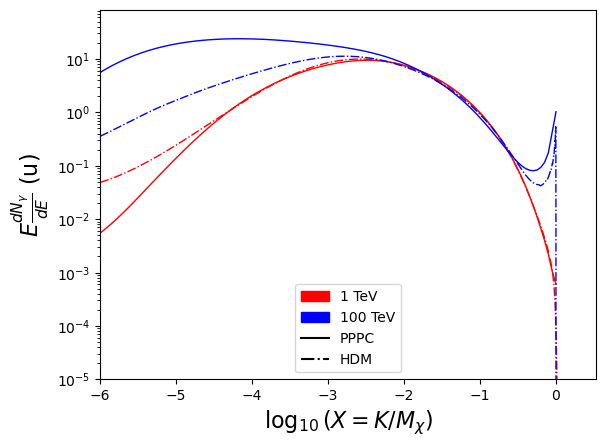
\includegraphics[scale=0.8]{figures/mtd_hawc_dm/pppc_vs_hdm.png}
    }
    \caption{Spectral hypotheses from PPPC \cite{Cirelli_2011} and HDM \cite{Rodd:HDM_spec} for DM annihilation: $\chi\chi \rightarrow W^-W^+$. Solid lines are spectral models with EW corrections from the PPPC. Dash-dot lines are spectral models from HDM. Red lines are models for $M_\chi = 1$ TeV. Blue lines represent models for $M_\chi = 100$ TeV.}
    \label{fig:pppc_vs_hdm}
\end{figure}

\Cref{fig:pppc_vs_hdm} demonstrates the impact of changes implemented in HDM on DM
annihilation to W bosons.
A class in astromodels was developed to include HDM and is aptly named \texttt{HDMSpectra} within \texttt{DM\_models.py}.
The SM DM annihilation channels studied here are $\chi\chi \rightarrow$:
\begin{itemize}
    \item[] $e^+e^-$, $\mu^+\mu^-$, $\tau^+\tau^-$,$b\bar{b}$, $t\bar{t}$, $gg$, $W^+W^-$, $ZZ$, $c\bar{c}$, $u\bar{u}$, $d\bar{d}$, $s\bar{s}$, $\nu_e \overline{\nu_e}$, $\nu_\mu \overline{\nu_\mu}$, $\nu_\tau \overline{\nu_\tau}$, $\gamma\gamma$, $hh$.
\end{itemize}
For $\gamma\gamma$ and $ZZ$, a substantial fraction of the signal photons are expected to have $E_\gamma = m_\chi$ \cite{Rodd:HDM_spec}.
This introduces a $\delta$-function in the tested spectra, referred to as a spectral line, that is much narrower than the energy resolution of the HAWC detector.
To ensure that this feature is not lost in the likelihood fits, the `line' feature is convolved with a Gaussian kernel with a $1\sigma$ width of $0.05 \cdot m_\chi$ and total kernel window of $\pm4\sigma$.
The kernel width was chosen based on the choices made from HAWC's previous gamma-line study \cite{HAWC_dm_gammalines} and the observed energy resolution of the NN energy estimator \cite{100TEV_Crab_HAWC}.
This differs from HAWC's previous line study where 30\% of HAWC's energy resolution was used for the kernel \cite{HAWC_dm_gammalines}.
The NN energy estimator's improved energy resolution compared to $f_\mathrm{hit}$ at low gamma-ray energy enables narrower kernels \cite{Rodd:HDM_spec} (see \cref{sec:hawc_nn}).
The annihilation spectra after Gaussian smoothing for $\chi\chi \rightarrow \gamma\gamma$ and $ZZ$ spectral hypotheses are shown in \cref{fig:hdm_gamma_lines}.
We did not explore how well we reconstruct injected signal events for various kernels widths.
This is a systematic that should be tested before publication in a journal.
Spectral models for the remaining annihilation channels are plotted for each $m_\chi$ in \Cref{fig:apdx_mtd_spectra}.

\begin{figure}[h]
    \centering{
    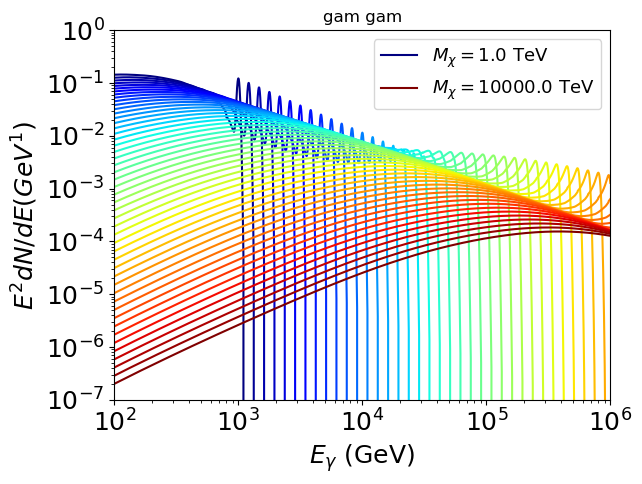
\includegraphics[scale=0.5]{figures/mtd_hawc_dm/hdm_gammagamma.png}
    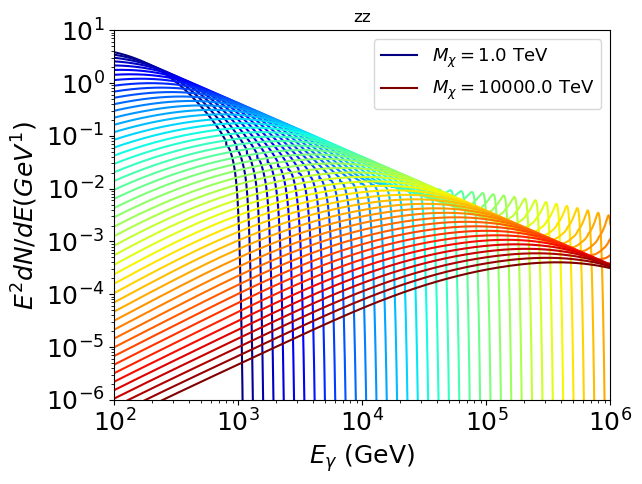
\includegraphics[scale=0.5]{figures/mtd_hawc_dm/hdm_zz.png}
    }
    \caption{Photon spectra for $\chi\chi \rightarrow \gamma\gamma$ (left) and $\chi\chi \rightarrow ZZ$ (right) after Gaussian convolution of line features. Both spectra have $\delta$-features at photon energies equal to the DM mass. Bluer lines are annihilation spectra with lower DM mass. Redder lines are spectra from larger DM mass. All spectral models are sourced from the Heavy Dark Matter models \cite{Rodd:HDM_spec}. Axes are drawn roughly according to the energy sensitivity of HAWC.}
    \label{fig:hdm_gamma_lines}
\end{figure}

%%%%%%%%%%%%%%%%%%%%%%%%%%%%%%%%%%%%%%%%%%%%%%%%%%
\subsection{\J Astrophysical Components}\label{sec:mtd_spatialmodel}
%%%%%%%%%%%%%%%%%%%%%%%%%%%%%%%%%%%%%%%%%%%%%%%%%%

The J-factor profiles for each source are imported from Louis Strigari et al. (referred to with \LS) \cite{DM_Strigari20}.
The \LS catalog fits a Navarro–Frenk–White (NFW) \cite{NFWProfile} spatial DM distributions to the dSphs which has a DM density of
\nfwProfile
$\rho_0$ and the scale radius, $R_s$ are free parameters fit for each dSph.
$r$ is the distance from the center of the dSph.
Because the \LS catalog uses fewer parameters for the DM density fits, they are able to fit on ultra-faint dSphs.
This increases the number of available profiles to 43.
The updated catalog was considered useful for a future combination with the IceCube neutrino observatory, and is a significant reason we selected this catalog.

Profiles in $\frac{d\J}{d\Omega} (\theta)$ up to an angular separation $\theta = 0.5^{\circ}$ were provided directly by the authors.
Map generation from these profiles were almost identical to \cref{sec:gd_spatialmodel} except that a higher order trapezoidal integral was used for the normalization of the square, uniformly-spaced map:
\TrapIntegral
$p$ is the angular side of one pixel in the map.
$w_{i,j}$ is a weight assigned the following ways:
\begin{itemize}
    \item[] $w_{i,j} = 1$ if $(\theta_{i,j}, \phi_{i,j})$ is fully within the region of integration
    \item[] $w_{i,j} = 1/2$ if $(\theta_{i,j}, \phi_{i,j})$ is on an edge of the region of integration
    \item[] $w_{i,j} = 1/4$ if $(\theta_{i,j}, \phi_{i,j})$ is on a corner of the region of integration
\end{itemize}
\Cref{fig:ls20_jfac_maps} shows the median and $\pm1\sigma$ maps used as input for this DM annihilation study.

\begin{figure}[t]
    \centering{
    \begin{tabular}{cccc}
        &
        $-1 \sigma$ &
        Median &
        $+1 \sigma$ \\

        \rotatebox[origin=c]{90}{Coma Berenices} &
        \raisebox{-.5\height}{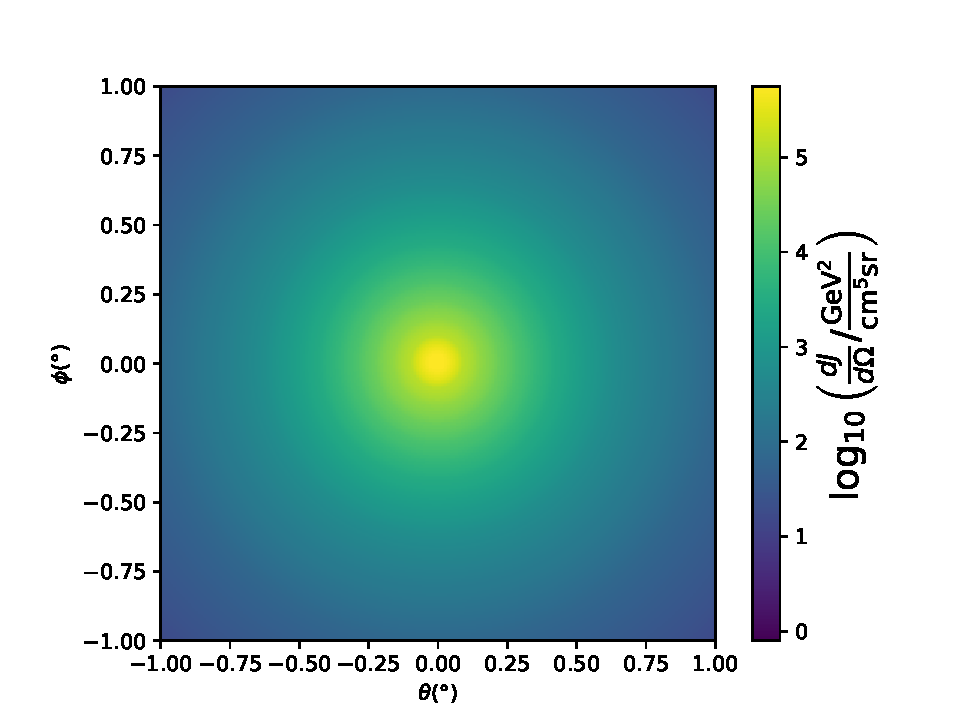
\includegraphics[scale=0.275]{figures/mtd_hawc_dm/ComaBerenices_Jm1_plot.pdf}} &
        \raisebox{-.5\height}{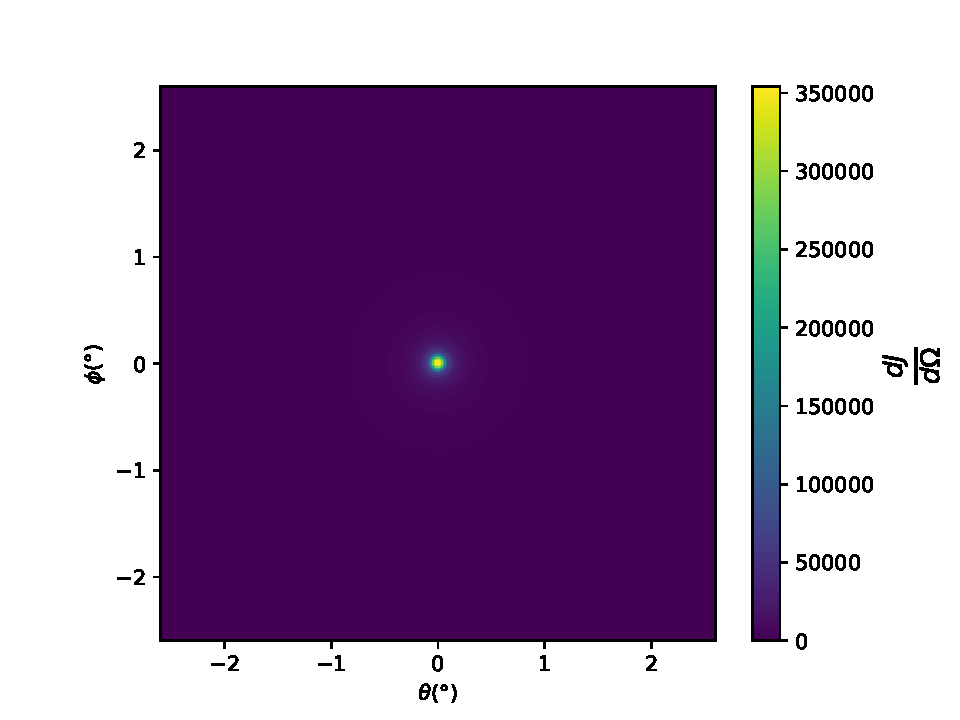
\includegraphics[scale=0.275]{figures/mtd_hawc_dm/ComaBerenices_J_plot.pdf}} &
        \raisebox{-.5\height}{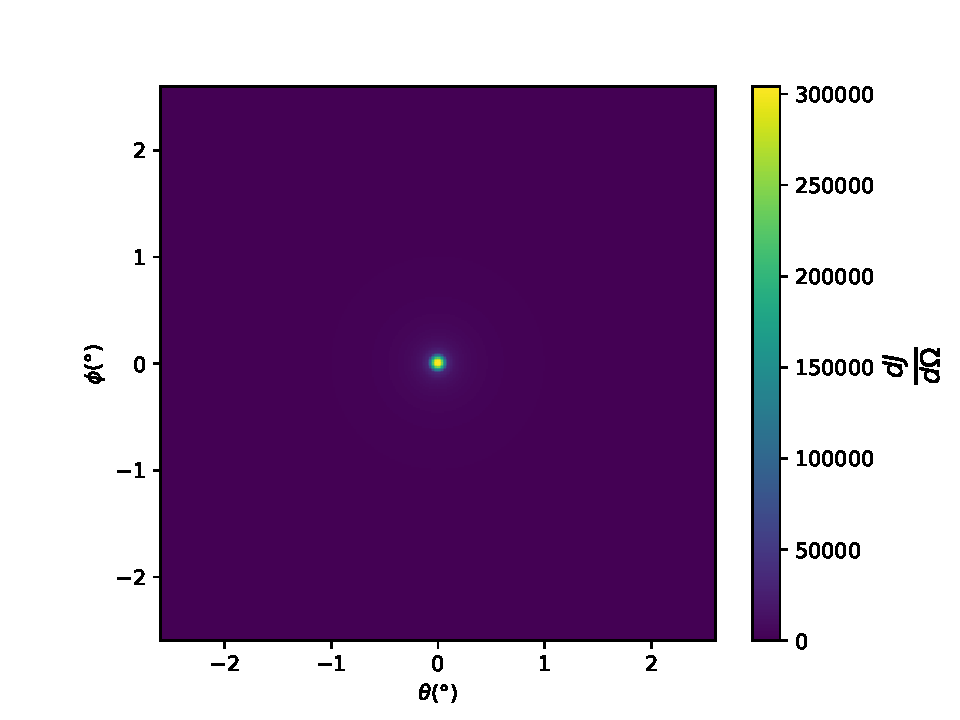
\includegraphics[scale=0.275]{figures/mtd_hawc_dm/ComaBerenices_Jp1_plot.pdf} }\\

        \rotatebox[origin=c]{90}{Segue1} &
        \raisebox{-.5\height}{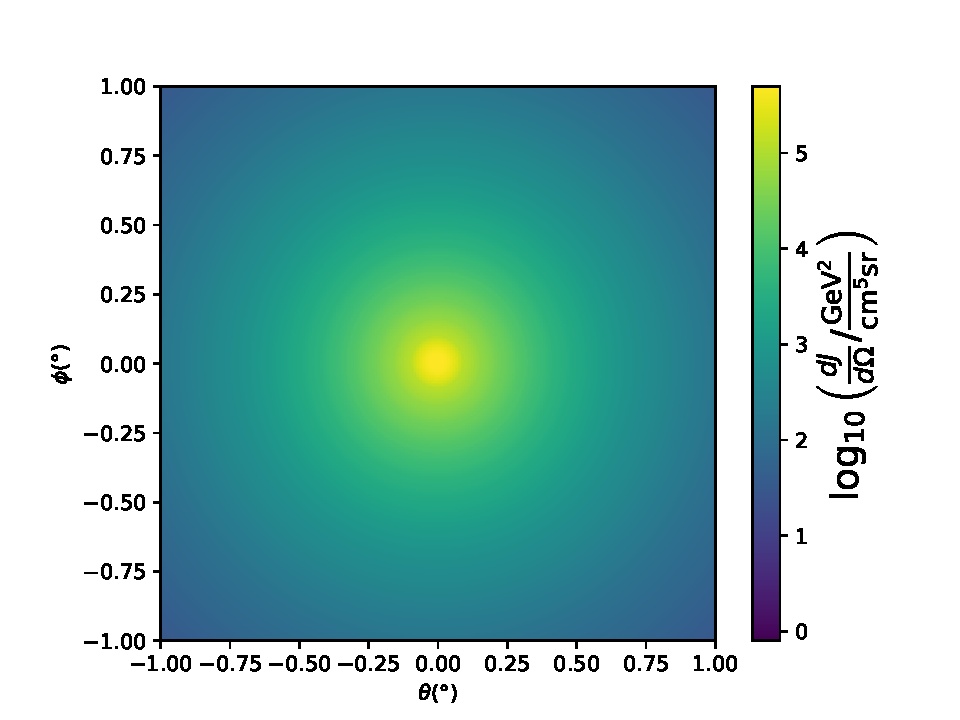
\includegraphics[scale=0.275]{figures/mtd_hawc_dm/Segue1_Jm1_plot.pdf}} &
        \raisebox{-.5\height}{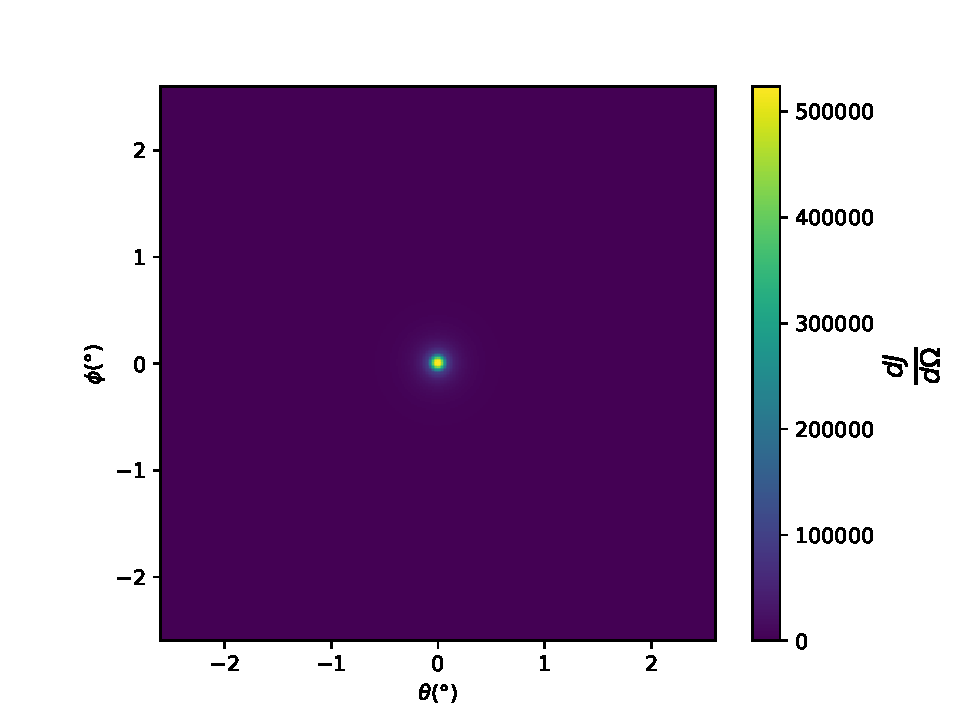
\includegraphics[scale=0.275]{figures/mtd_hawc_dm/Segue1_J_plot.pdf}} &
        \raisebox{-.5\height}{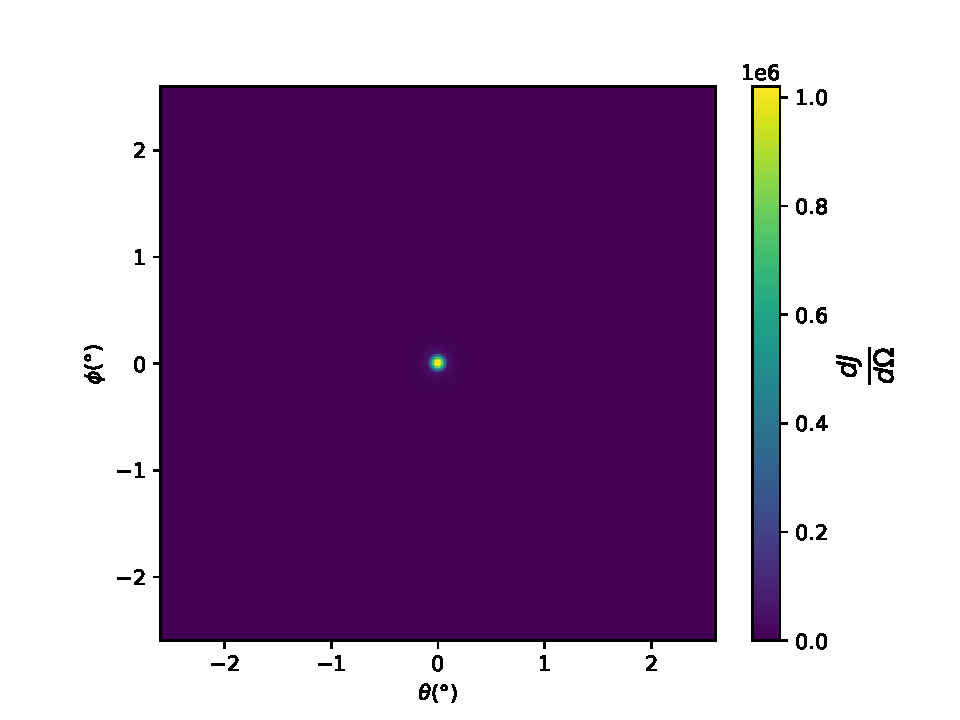
\includegraphics[scale=0.275]{figures/mtd_hawc_dm/Segue1_Jp1_plot.pdf}} \\

        \rotatebox[origin=c]{90}{Sextans} &
        \raisebox{-.5\height}{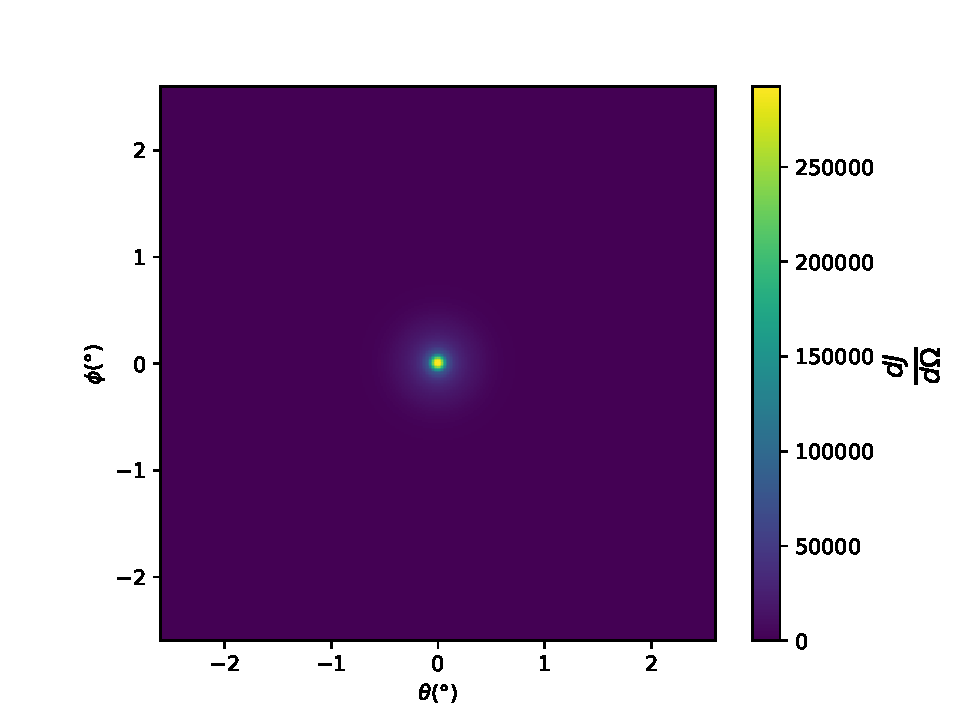
\includegraphics[scale=0.275]{figures/mtd_hawc_dm/Sextans_Jm1_plot.pdf}} &
        \raisebox{-.5\height}{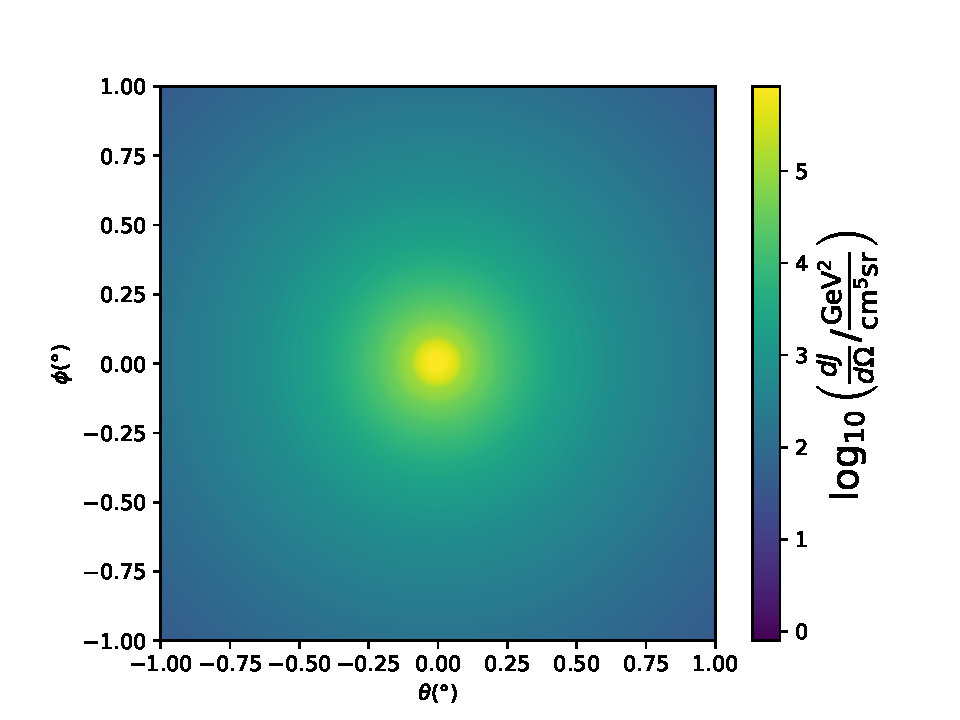
\includegraphics[scale=0.275]{figures/mtd_hawc_dm/Sextans_J_plot.pdf}} &
        \raisebox{-.5\height}{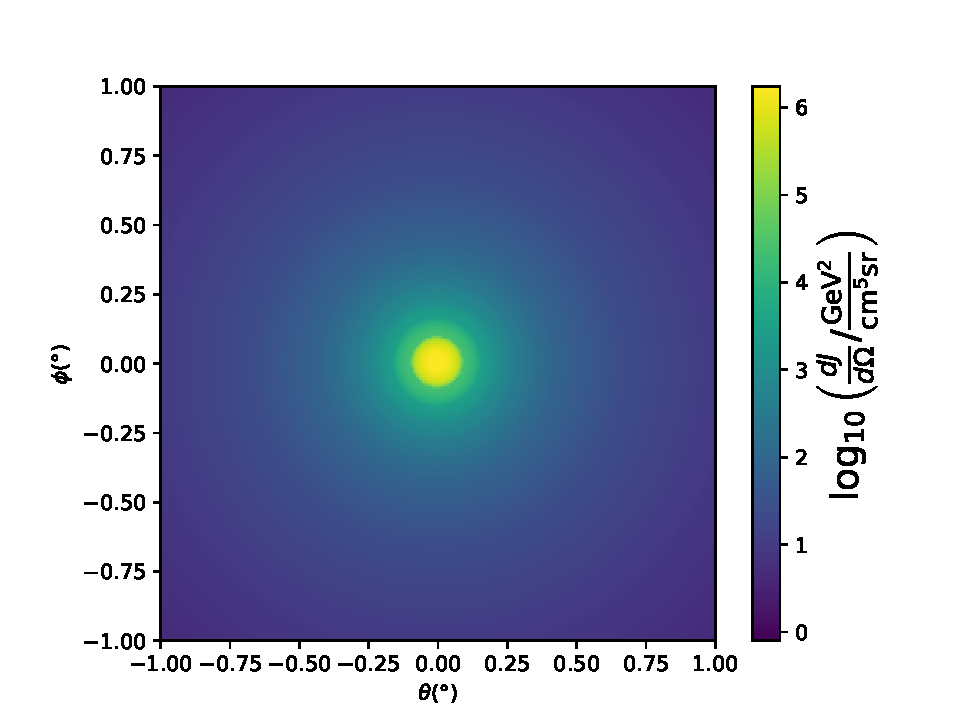
\includegraphics[scale=0.275]{figures/mtd_hawc_dm/Sextans_Jp1_plot.pdf}} \\
    \end{tabular}
    }
    \caption{$\frac{d\J}{d\Omega}$ maps for Coma Berenices, Segue1, and Sextans. Columns are divided for the $\pm1 \sigma$ uncertainties in $d\J/d\Omega$ around the mean value from \LS \cite{DM_Strigari20}. Origin is centered on the specific dwarf spheroidal galaxies (dSph). $\theta$ and $\phi$ axes are the angular separation from the center of the dwarf. Profiles are truncated at 1$^\circ$ and flattened beyond.}
    \label{fig:ls20_jfac_maps}
\end{figure}

%%%%%%%%%%%%%%%%%%%%%%%%%%%%%%%%%%%%%%%%%%%%%%%%%%
\subsection{Source Selection and Annihilation Channels}\label{sec:mtd_srcs_y_chan}
%%%%%%%%%%%%%%%%%%%%%%%%%%%%%%%%%%%%%%%%%%%%%%%%%%

HAWC's sources for this multithreaded analysis include Coma Berenices, Segue 1, and Sextans.
\LS estimated the DM distributions of 43 sources in its publication, however only 4 of the best fit profiles within HAWC's field of view were provided at the time this thesis was written.
A full description of each source used in this analysis is found in \cref{tab:mtd_J_factor}.

\begin{table}[b]
\centering
    \small{\begin{tabular}{cccc}
    \hline
    \hline
    \CellTopTwo{}
    Name & Distance & $l, b$ & $\log_{10}J$~(\LS set)\\
    & \scriptsize{(kpc)} &  \scriptsize{($\degree$)} & \scriptsize{$\log_{10}(\mathrm{GeV}^2 \mathrm{cm}^{-5}\mathrm{sr})$} \\
    \hline
    \CellTopTwo{}
    Coma Berenices & $44$ & $241.89,\: 83.61$ & $19.00^{+0.36}_{-0.35}$ \\
    \CellTopTwo{}
    Segue I & $23$ & $220.48,\: 50.43$ & $19.12^{+0.49}_{-0.58}$ \\
    \CellTopTwo{}
    Sextans & $86$ & $243.50,\: 42.27$ & $17.73^{+0.13}_{-0.12}$ \\
    \hline
    \hline
    \CellTopTwo{}
\end{tabular}}
    \caption{Summary of the relevant properties of the dSphs used in the present work. Column 1 lists the dSphs. Columns 2 and 3 present their heliocentric distance and galactic coordinates, respectively. Column 4 reports the \J-factors of each source given from the \LS studies and estimated $\pm 1\sigma$ uncertainties. The values $\log_{10}J$~(\LS set) \cite{DM_Strigari20} correspond to the mean \J-factor values  for a source extension truncated at $0.5^\circ$.}
    \label{tab:mtd_J_factor}
\end{table}

This analysis improves on \Cref{sec:glory_duck} in the following ways.
Previously, the particle physics model used for gamma-ray spectra from DM annihilation was from the PPPC \cite{Cirelli_2011} which missed important considerations relevant for the neutrino sector.
HDM is used to account for this shortfall \cite{Rodd:HDM_spec}.
HDM also models DM to the Planck scale which permits HAWC to probe PeV scale DM.
For this study, we sample DM masses: $1$ TeV - $10$ PeV with 6 mass bins per decade in DM mass.
In the case of line spectra ($\chi\chi \rightarrow \gamma\gamma$, or $ZZ$), we double the mass binning to 12 DM mass bins per decade in DM mass.

\LS published 25 sources' \J-factors within HAWC's field of view.
Additionally, NFW \cite{NFWProfile} DM distributions have fewer parameters than Zhao \cite{Zhao:1995cp}, so \LS fits ultra-faint dwarves which expands the number of sources.
However, all sources were not provided by the authors in time for the completion of this dissertation.
Draco was provided by the authors.
However, Draco is not included in this study as the PSF of the bins at its declination were wider than what is reasonable for a point source analysis.
Finally, the gamma-ray ray dataset is much larger.
The study performed here analyzes 2565 days of data compared to 1017 days analyzed in \Cref{sec:glory_duck}.

%%%%%%%%%%%%%%%%%%%%%%%%%%%%%%%%%%%%%%%%%%%%%%%%%%%%%%%%%%%%%
\section{Likelihood Methods} \label{sec:mtd_ll_methods}
%%%%%%%%%%%%%%%%%%%%%%%%%%%%%%%%%%%%%%%%%%%%%%%%%%%%%%%%%%%%%

These are identical to \cref{sec:gd_hawc_llh} and no additional changes are made to the likelihood.
Bins in this analysis are expanded to include HAWC's NN energy estimator.

%%%%%%%%%%%%%%%%%%%%%%%%%%%%%%%%%%%%%%%%%%%%%%%%%%%%%%%%%%%%%
\section{Computational Methods: Multithreading} \label{sec:mtd_comp_methods}
%%%%%%%%%%%%%%%%%%%%%%%%%%%%%%%%%%%%%%%%%%%%%%%%%%%%%%%%%%%%%

Previously, as in \cref{sec:gd_analysis}, the likelihood was minimized for one model at a time.
One model in this case representing a DM annihilation channel (\texttt{CHAN}), DM mass ($m_\chi$), and dSph (\texttt(SOURCE)).
In an effort to conserve human and CPU time, jobs submitted for high performance computing contained a list of $m_\chi$ to iterate over for likelihood fitting.
Jobs were then trivially parallelized for each permutation of the two lists: \texttt{CHANS} and \texttt{SOURCES}.
The lists for \texttt{CHANS} and \texttt{SOURCES} are found in \cref{sec:mtd_particlephysics,tab:mtd_J_factor}, respectively.
Initially, 11 $m_\chi$ were serially sampled for one job defined by a [\texttt{CHAN}, \texttt{SOURCE}] tuple.
Computing the likelihoods would take between 1.5 to 2 hrs, stochastically, for a job.
We expect to compute likelihoods for data and 300 Poisson background trials.
The estimated CPU time based on the above for all \texttt{CHAN} (N = 17) and \texttt{SOURCE} (M = 25) was estimated to be $127,925$ jobs.
In total, $1,407,175$ likelihood fits and profiles would be computed for the 11 mass bins we wished to study.
The estimated CPU time ranged between $8$k CPU days to $10$k CPU days.
Human time is more challenging to estimate as job allocation is stochastic and highly dependent on what other users are submitting.
Yet, it is unlikely that all jobs would run simultaneously.
Therefore, we can expect human time to be about as long as was seen in \Cref{sec:glory_duck}, which was on the order of months to fully compute a smaller analysis.
A visual aid to describe how jobs were organized is provided in \cref{fig:mtd_gd_workflow}.

\begin{figure}[h]
    \centering{
        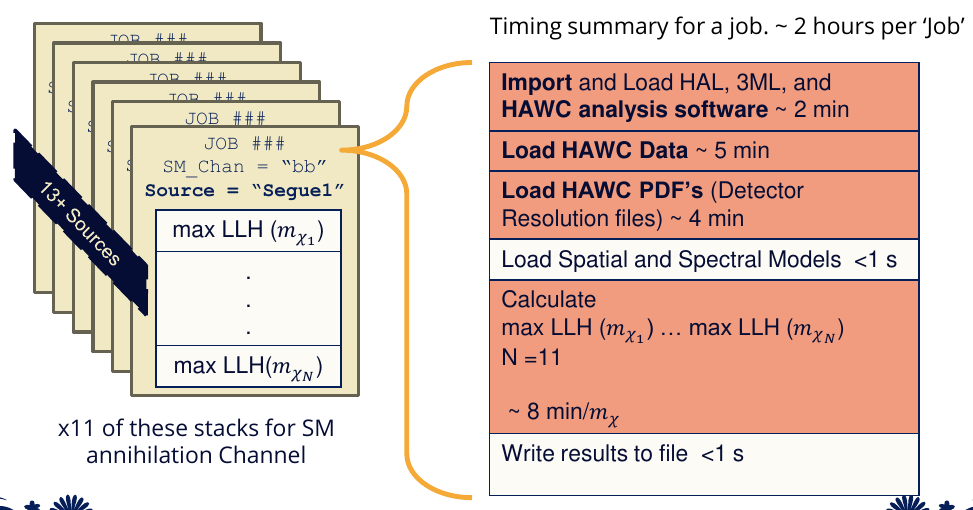
\includegraphics[scale=0.6]{figures/mtd_hawc_dm/gd_workflow.png}
    }
    \caption{Infographic on how jobs and DM computation was organized in \Cref{sec:gd_analysis}. Jobs were built for each permutation of \texttt{CHANS} and \texttt{SOURCES} shown by the left block in the figure. Each job, which took on the order 2 hrs to compute, had the following work flow: 1. Import HAWC analysis software, 2 min to run. 2. Load HAWC count maps, 5 min to run. 3. Load HAWC energy and spatial resolutions, 4 min. 5. Load DM spatial source templates and spectral models, less than 1 s. 6. Perform likelihood fit on data and model, about 8 min per DM mass. 7. Write results to file, less than 1s.}
    \label{fig:mtd_gd_workflow}
\end{figure}

The computational needs for this next generation DM analysis are extreme and is unlike other analyses performed on HAWC.
It became clear that there was a lot to gain from optimizing how the likelihoods are computed.
This section discusses how multi-threading was applied to solve and reduce HAWC's computing of likelihoods for large parameter spaces like in DM searches.

%%%%%%%%%%%%%%%%%%%%%%%%%%%%%%%%%%%%%%%%%%%%%%%%%%%%%%%%%%%%%
\subsection{Relevant Foundational Information}\label{sec:mtd_foundation}
%%%%%%%%%%%%%%%%%%%%%%%%%%%%%%%%%%%%%%%%%%%%%%%%%%%%%%%%%%%%%

The profiling of the likelihood for HAWC is done via gradient descent where the normalization of \Cref{eq:id_dm_flux} (linearly correlated with \sv) is rescaled in the descent.
Additionally, we sample the likelihood space for a defined list of \sv's described in \Cref{sec:gd_joint_llh}.
The time to compute these values is not predictable or consistent because many variables can change across the full model-space.
Comprehensively, these variables are:
\begin{itemize}
    \item $m_\chi$ : DM rest mass
    \item \texttt{CHAN} : DM annihilation channel in SM.
    \item \texttt{SOURCE} : dSph. Involves a spatial template AND coordinate in HAWC data.
    \item \sv: Proportional to the flux normalization and free parameter in the likelihood fit.
\end{itemize}
Therefore, an asynchronous, functional-parallel coding pattern was developed.
Asynchronous means the instructions within a function are independent and permitted to be out of sync with sibling computations.
Functional-parallel means that instructions are the subject of parallelization rather than threading the likelihood computation.
This is close to trivial parallelization seen in \cref{fig:mtd_gd_workflow} except that jobs are joined in the loading stages (software, data, and detector resolution loading).
Multiple asynchronous threads are expected to reduce total serial processing time and total overhead across the entire project in addition to saving human time.

\begin{figure}[h]
    \centering{
        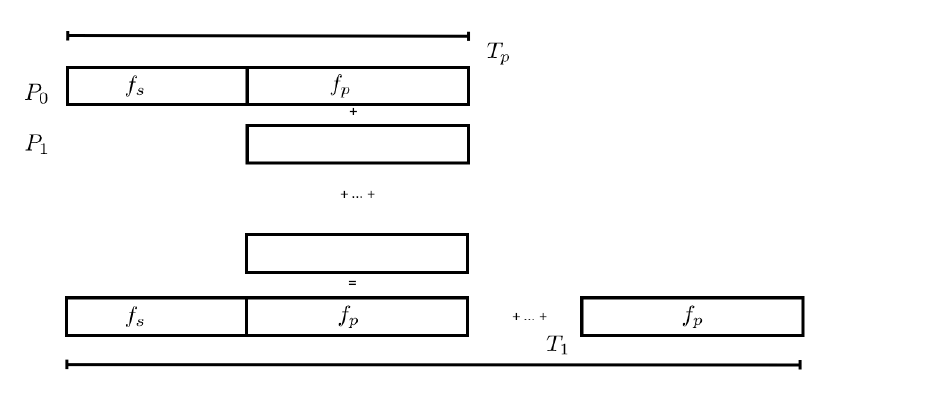
\includegraphics[scale=0.65]{figures/mtd_hawc_dm/gufstafson_coding_pattern.png}
    }
    \caption{Graphic of Gustafson parallel coding pattern. $f_s$ is the fraction of a program, in time, spent on serial computation. $f_p$ is the fraction of computing time that is parallelizable. $T_p$ is the total time for a parallel program to run. $T_1$ is the total time for a parallel program to run if only 1 processor is allocated. $P_N$ is the $N$-th processor where it's row is the computation the processor performs. The Gustafson pattern is most similar to what is implemented for this analysis. Figure is pulled from \cite{ArtofHPC}.}
    \label{fig:mtd_gufsta}
\end{figure}

A way to measure and compare the expected speedup and efficiency gain is needed for this asynchronous coding pattern.
Inspiration for timing measurement was pulled from \cite{ArtofHPC} and used \textit{Amdahl's law with hybrid programming}.
Hybrid programming meaning that the computation is a mix of distributed and shared memory programming.
Assuming the code is fully parallelizable over $p$ processors and $c$ threads, the ideal speedup is simply $pc$, and ideal run-time is $T_1/(pc)$.
$T_1$ is the total time for a parallel program to run if only 1 processor is allocated.
However, the coding pattern contains some amount of unavoidable serial computation, as shown in \Cref{fig:mtd_gufsta}.
In this case, the run time, $T_{p,c}$, is estimated to be
\amdahl
$F_s$ is the fraction of CPU time dedicated to serial computation.
The expected speedup, $S_{p,c}$, is
\amdahlSpeed
From \Cref{eq:amdahlSpeed}, we can see that the speed-up scales with $p/F_s$.
We are free to minimize $F_s$ asymptotically by enlarging the total models that are submitted to the thread pool, thereby shrinking the CPU fraction dedicated to serial operation.
We are also free to define exactly how many threads and processors we utilize, yet eventually hit a hard cap at the hardware available on our computing cluster.
HAWC uses Intel Xeon\texttrademark processors with 48 cores and 96 threads.
We see that a successful code will scale well as the expected speedup is inversely correlated with $F_s$.
As the total number of models sampled grows, the speedup will also.

%%%%%%%%%%%%%%%%%%%%%%%%%%%%%%%%%%%%%%%%%%%%%%%%%%%%%%%%%%%%%
\subsection{Implementation}\label{sec:mtd_implementation}
%%%%%%%%%%%%%%%%%%%%%%%%%%%%%%%%%%%%%%%%%%%%%%%%%%%%%%%%%%%%%

\begin{figure}[h]
    \centering{
        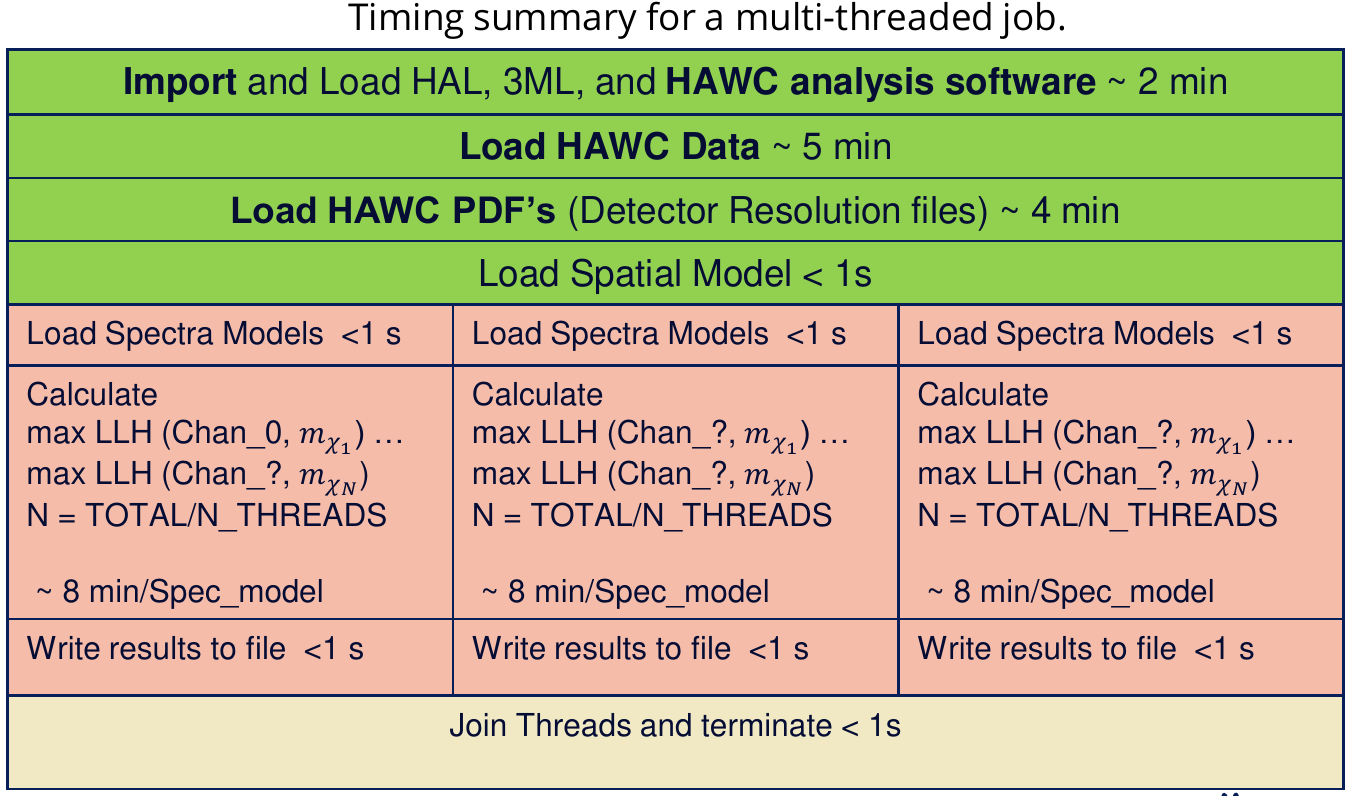
\includegraphics[scale=0.4]{figures/mtd_hawc_dm/mult-threaded_hawc.png}
    }
    \caption{Task chart for one multithreaded job developed for this project. Green blocks indicate a shared resource across the threads AND computation performed serially. Red blocks indicate functional parallel processing within each thread. 3 threads are represented here, yet many more can be employed during the full analysis. Jobs are defined by the \texttt{SOURCE} as these require unique maps to be loaded into the likelihood estimator. The $m_\chi$, \texttt{CHAN}, and \sv~variables are entered into the thread pool and allocated as evenly as possible across the threads.}
    \label{fig:mtd_multithreads}
\end{figure}

The multithreaded code was written in Python3 and is documented in the \href{https://gitlab.com/hawc-observatory/sandboxes/salaza82/dark\_matter\_hawc}{\texttt{dark\_matter\_hawc} repository} within the script named \texttt{mpu\_analysis.py}.
A version of the script as of April 15 is also provided in \Cref{sec:apx_mpu_script}.
It has many dependencies including the HAWC analysis software.
\Cref{fig:mtd_multithreads} displays the workflow of a job with 3 threads.
Within a job, \texttt{SOURCE} is kept fixed and \texttt{CHANS} remains 17 elements long.
More $m_\chi$ are sampled from 11 bins up to 49 (for $\gamma\gamma$ and $ZZ$) and 25 (for remaining \texttt{CHANS}) which amounts to 12 or 6 mass bins per decade.
$m_\chi$ and \texttt{CHANS} are permuted into a 473 element list which is split evenly across N threads where N is [2, 8, 16].
For each $m_\chi$-\texttt{CHAN} tuple, 1001 \sv~values are sampled in the likelihood, and the value of \sv~that maximizes the likelihood is found.
Although rare, fits that failed are handled on a case by case basis.

%%%%%%%%%%%%%%%%%%%%%%%%%%%%%%%%%%%%%%%%%%%%%%%%%%%%%%%%%%%%%
\subsection{Performance}\label{sec:mtd_performance}
%%%%%%%%%%%%%%%%%%%%%%%%%%%%%%%%%%%%%%%%%%%%%%%%%%%%%%%%%%%%%

\begin{table}[h]
    \centering
    {\begin{tabular}{c ? c  c  c  c }
    & \multicolumn{4}{c}{$T_{p,c}$ (hr:min:s)} \\
    \hline
    \hline
    M Tasks & $T_{1,1}$ & $T_{1,2}$ & $T_{1,8}$ & $T_{1,16}$ \\
    \hline
    50 & 1:40:37.5 & 0:52:43.7 & 0:19:13.8 & 0:13:44.0 \\
    74 & 2:22:30.0 & 1:15::00.6 & 0:25:21.3 & 0:15:49.8 \\
    100 & (3:07:51.9) & 1:40:10.5 & 0:30:44.4 & 0:20:01.4 \\
    200 & (6:02:20.6) & - & &  \\
    473 & (13:58:40.3) & - & & 1:09:42.9 \\
    \end{tabular}}
    \caption{ Timing summaries for analyses for serial and multithreaded processes. M tasks is the number of functional-parallel tasks ran for the computation. $T_{p,c}$ is a single run time in hours:minutes:seconds for runs utilizing $p$ nodes and $c$ threads. Runs are run interactively on the same computer to maximize consistency. Empty entries are indicated with '-'. $(\cdot)$ entries are estimated entries extrapolated from data earlier in the column.}\label{tab:mtd_timing_study}
\end{table}

A significant reduction to wall time is needed for the dSphs analysis to run.
\Cref{tab:mtd_timing_study} shows the timing summaries for analyses of different sizes and thread counts.
Additionally, the efficiency gained when consolidating the serial loading of data is also apparent in our ability to study many more tasks in about the same amount of wall time as a smaller serial computation.
Trials represented in the table were run on an AMD Opteron\textsuperscript{\textregistered} processor 6344 with 48 cores, 2 threads per core; 2.6 GHz clock.
This is not the same architecture used for analysis on the HAWC computing cluster however they are similar enough that results shown here are reasonably representative of computing on the HAWC computing cluster.
\Cref{tab:mtd_timing_study} is used for the inferences and conclusions made in the following paragraphs.

First, we want to find $T_s$, the time of serial computation.
From \cref{fig:mtd_gufsta}, the timing for our coding pattern can be written as
\TimingAll
$M$ is the number of functional-parallel tasks (represented as column 1 of \cref{tab:mtd_timing_study}), and $t_p$ is the average time to complete a single parallel task.
$T^M_{1,1}$ is the total time for a parallel program to run if only 1 processor is allocated for M parallel task.
With two runs of different M ($M1$ and $M2$), we can use a system of equations to compute
% \TsfromMs
% We also extract $t_p$ using the same methods:
% \TpfromMs
% From \cref{tab:mtd_timing_study}, we set $M1 = 50$ and $M2 = 74$ and take their corresponding $T_{1,1}$ from the table to calculate $T_s$ and $t_p$.
\TsTp{803.1}{104.6}
Now, we have specific estimation for the fraction of serial computing time, $F_s$:
\specificFs{803.1}{104.6}
The maximum M for this study is 473 which evaluates to: $F_s = 0.016$ or 1.6\% of computing time.
\Cref{tab:mtd_speedup_study} shows the resulting speedups.
\begin{table}[h]
    \centering
    {\begin{tabular}{c c ? c c c}
    & \multicolumn{3}{c}{$S_{p,c}$} \\
    \hline
    \hline
    M Tasks & $F_s$ & $S_{1,2}$ & $S_{1,8}$ & $T_{1,16}$ \\
    \hline
    50  & & 1.90 [1.76] & 5.23 [4.14] & 6.35 [5.34] \\
    74  & & 1.90 [1.83] & 5.62 [4.82] & 9.00 [6.64] \\
    100 & & & & \\
    200 & & - & & \\
    473 & & - & & 1:09:42.9 \\
    \end{tabular}}
    \caption{ Speed up summaries for analyses for serial and multithreaded processes. M tasks is the number of functional-parallel tasks ran for the computation. $S_{p,c}$ is a single speedup comparison for runs utilizing $p$ nodes and $c$ threads. $[\cdot]$ are the estimated speedups calculated from \cref{tab:mtd_timing_study}, \cref{eq:specificFs}, and \cref{eq:amdahlSpeed}. Empty entries are indicated with '-'.}\label{tab:mtd_speedup_study}
\end{table}

A speedup that generally exceeds expectations from \cref{eq:amdahlSpeed} is seen for real trail runs.
There are also diminishing returns as the number of threads increases.
For small jobs with large $c$, both the expected and observed speedup are significantly smaller than $c$.
One thing not considered in \cref{eq:amdahlSpeed} is the time incurred via communication latency.
Communication latency increases with the number of threads and contributes to diminishing returns.
Additionally, these values are for single runs and do not consider the stochastic variation expected in a shared high performance computing resource.
Therefor, these results are not strictly conclusive, yet demonstrate the merits of multi-threading.
There is a lot to gain, and this new coding pattern will expand HAWC's analysis capabilities.

%%%%%%%%%%%%%%%%%%%%%%%%%%%%%%%%%%%%%%%%%%%%%%%%%%%%%%%%%%%%%
\section{Analysis Results}\label{sec:mtd_results}
%%%%%%%%%%%%%%%%%%%%%%%%%%%%%%%%%%%%%%%%%%%%%%%%%%%%%%%%%%%%%

Three of the 43 \LS dSphs are considered for the multithreaded analysis.
These dSph are analyzed for emission from DM annihilation according to the likelihood method described in \Cref{sec:gd_ll_methods}.
The three likelihood profiles are then stacked to synthesize a combined limit on the dark matter annihilation cross-section, \sv.
This combination is done for each of the 17 SM annihilation channels.
\Cref{fig:mtd_limits_1of2} and \cref{fig:mtd_limits_2of2} show the combined limits for all annihilation channels with HAWC's observations.
Test statistics of the best fit \sv~values for each $m_\chi$ and \texttt{CHAN} are shown in \cref{fig:mtd_TS_1of2} and \cref{fig:mtd_TS_2of2}.
These limits are compared to HAWC's Glory Duck limits from \cref{sec:hawc_results} and shown in \cref{fig:mtd_compare2gd} for all the DM annihilation channels studied for Glory Duck.
A full comparison is provided in \Cref{apdx:mtd_supp_figures} in \crefrange{fig:mtd_compare_ComaB}{fig:mtd_compare_Sextans}.
Here, we show updated limits for $\chi\chi \rightarrow$ \parpar{b}, \parpar{e}, \parpar{\mu}, \parpar{\tau}, \parpar{t}, $W^+W^-$, \pp{\gamma} and \pp{Z}.
For the first time ever, we show limits for $\chi\chi \rightarrow$ \parpar{c}, \parpar{s}, \parpar{u}, \parpar{d}, \parpar{\nu_e}, \parpar{\nu_\mu}, \parpar{\nu_\tau}, \pp{g}, and \pp{h}.

\begin{figure}[h]
\centering{
    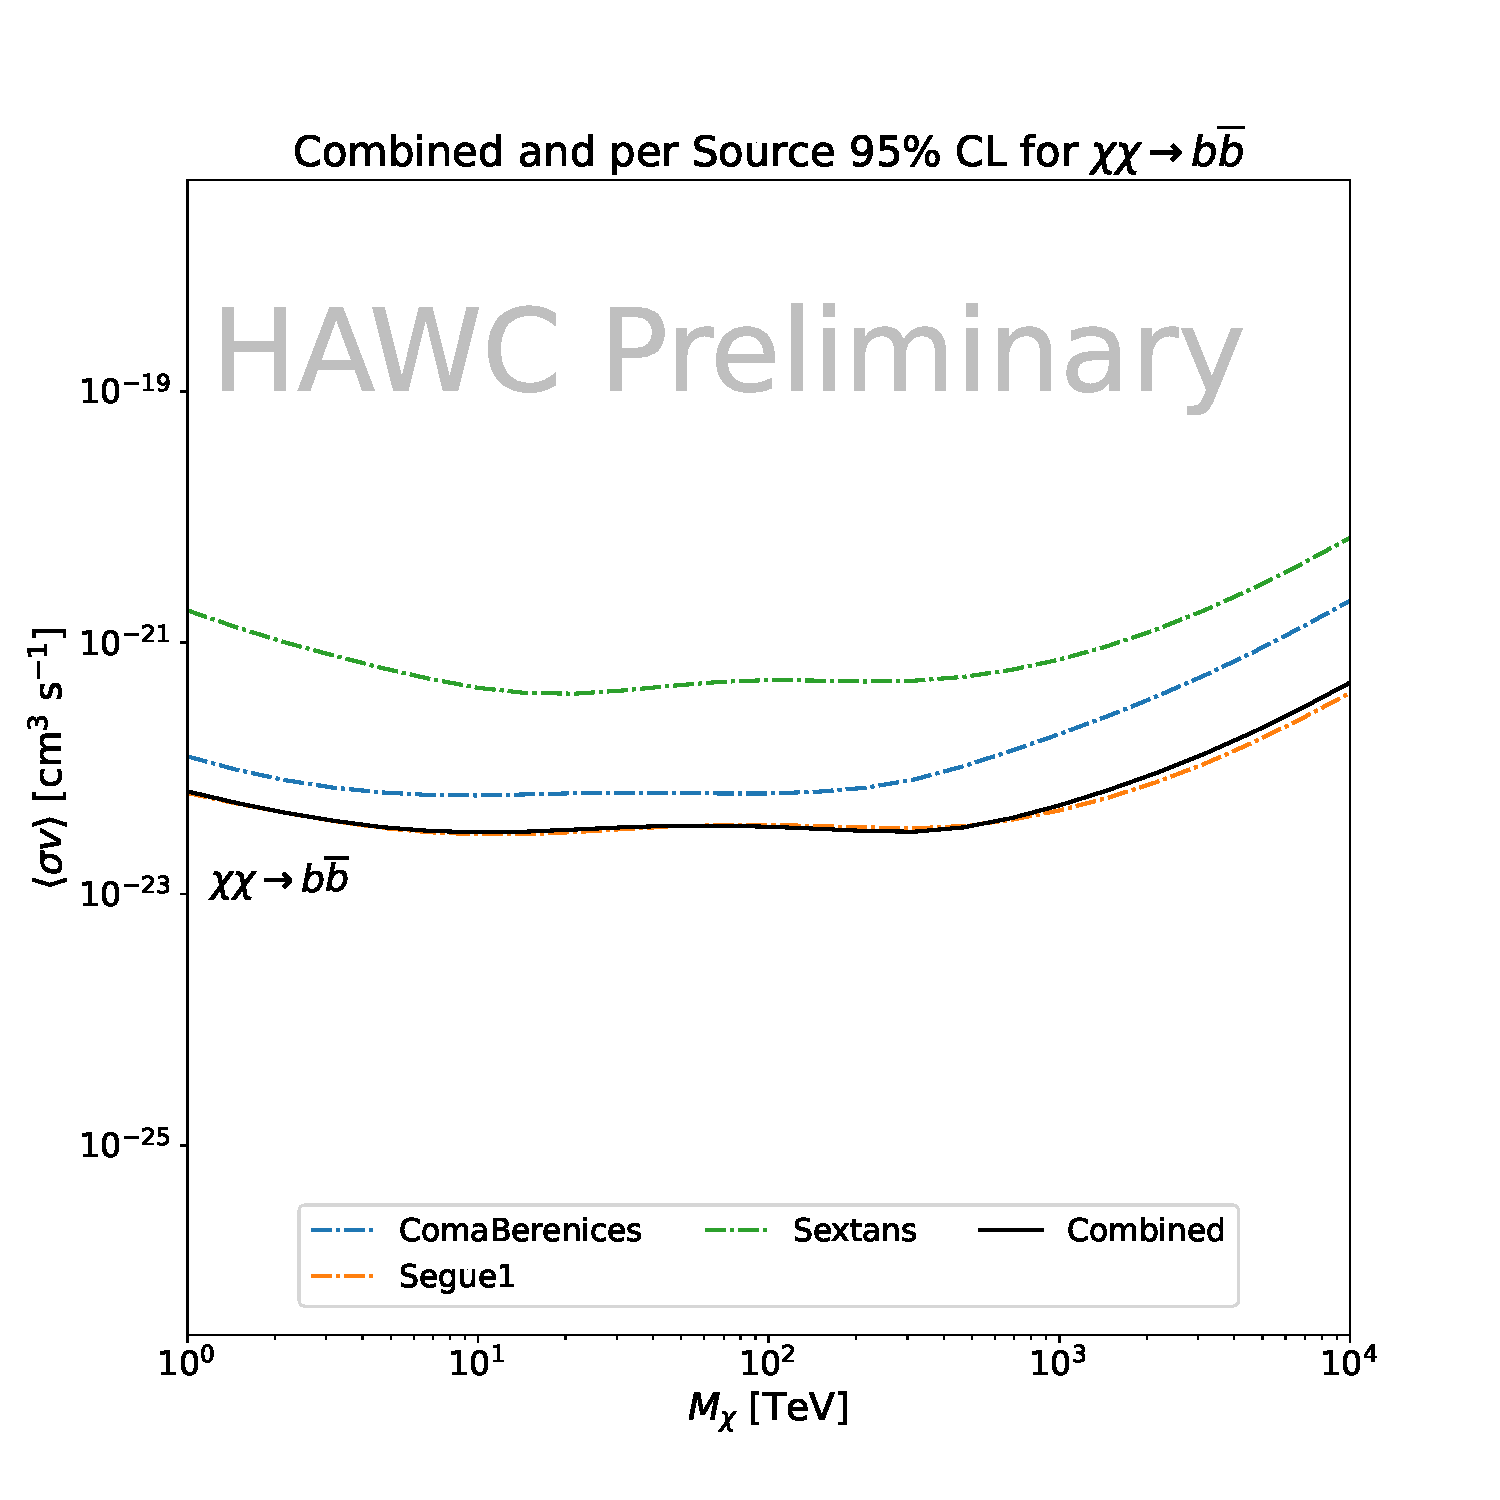
\includegraphics[scale=0.21]{figures/mtd_hawc_dm/results/Combined95_New_duck_bb_.pdf}
    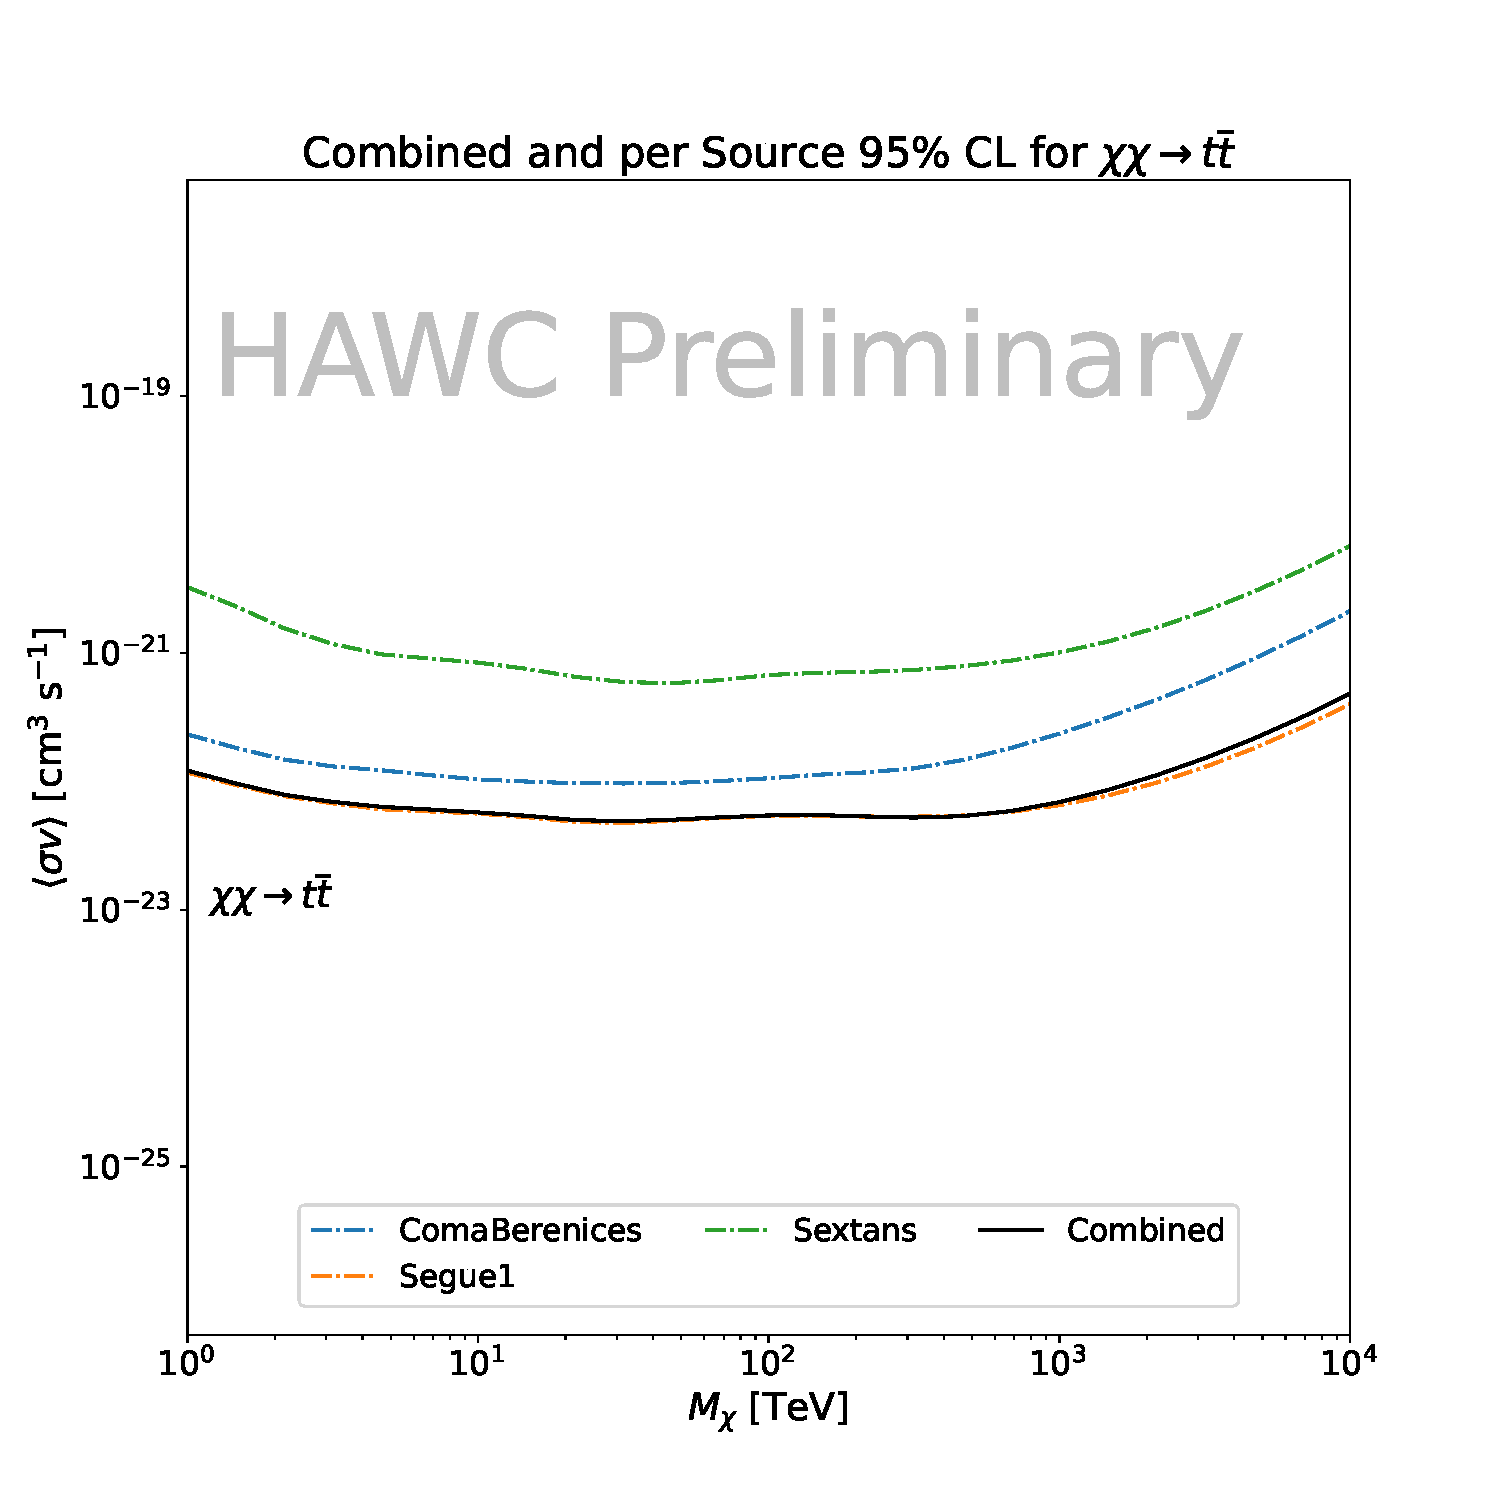
\includegraphics[scale=0.21]{figures/mtd_hawc_dm/results/Combined95_New_duck_tt_.pdf}
    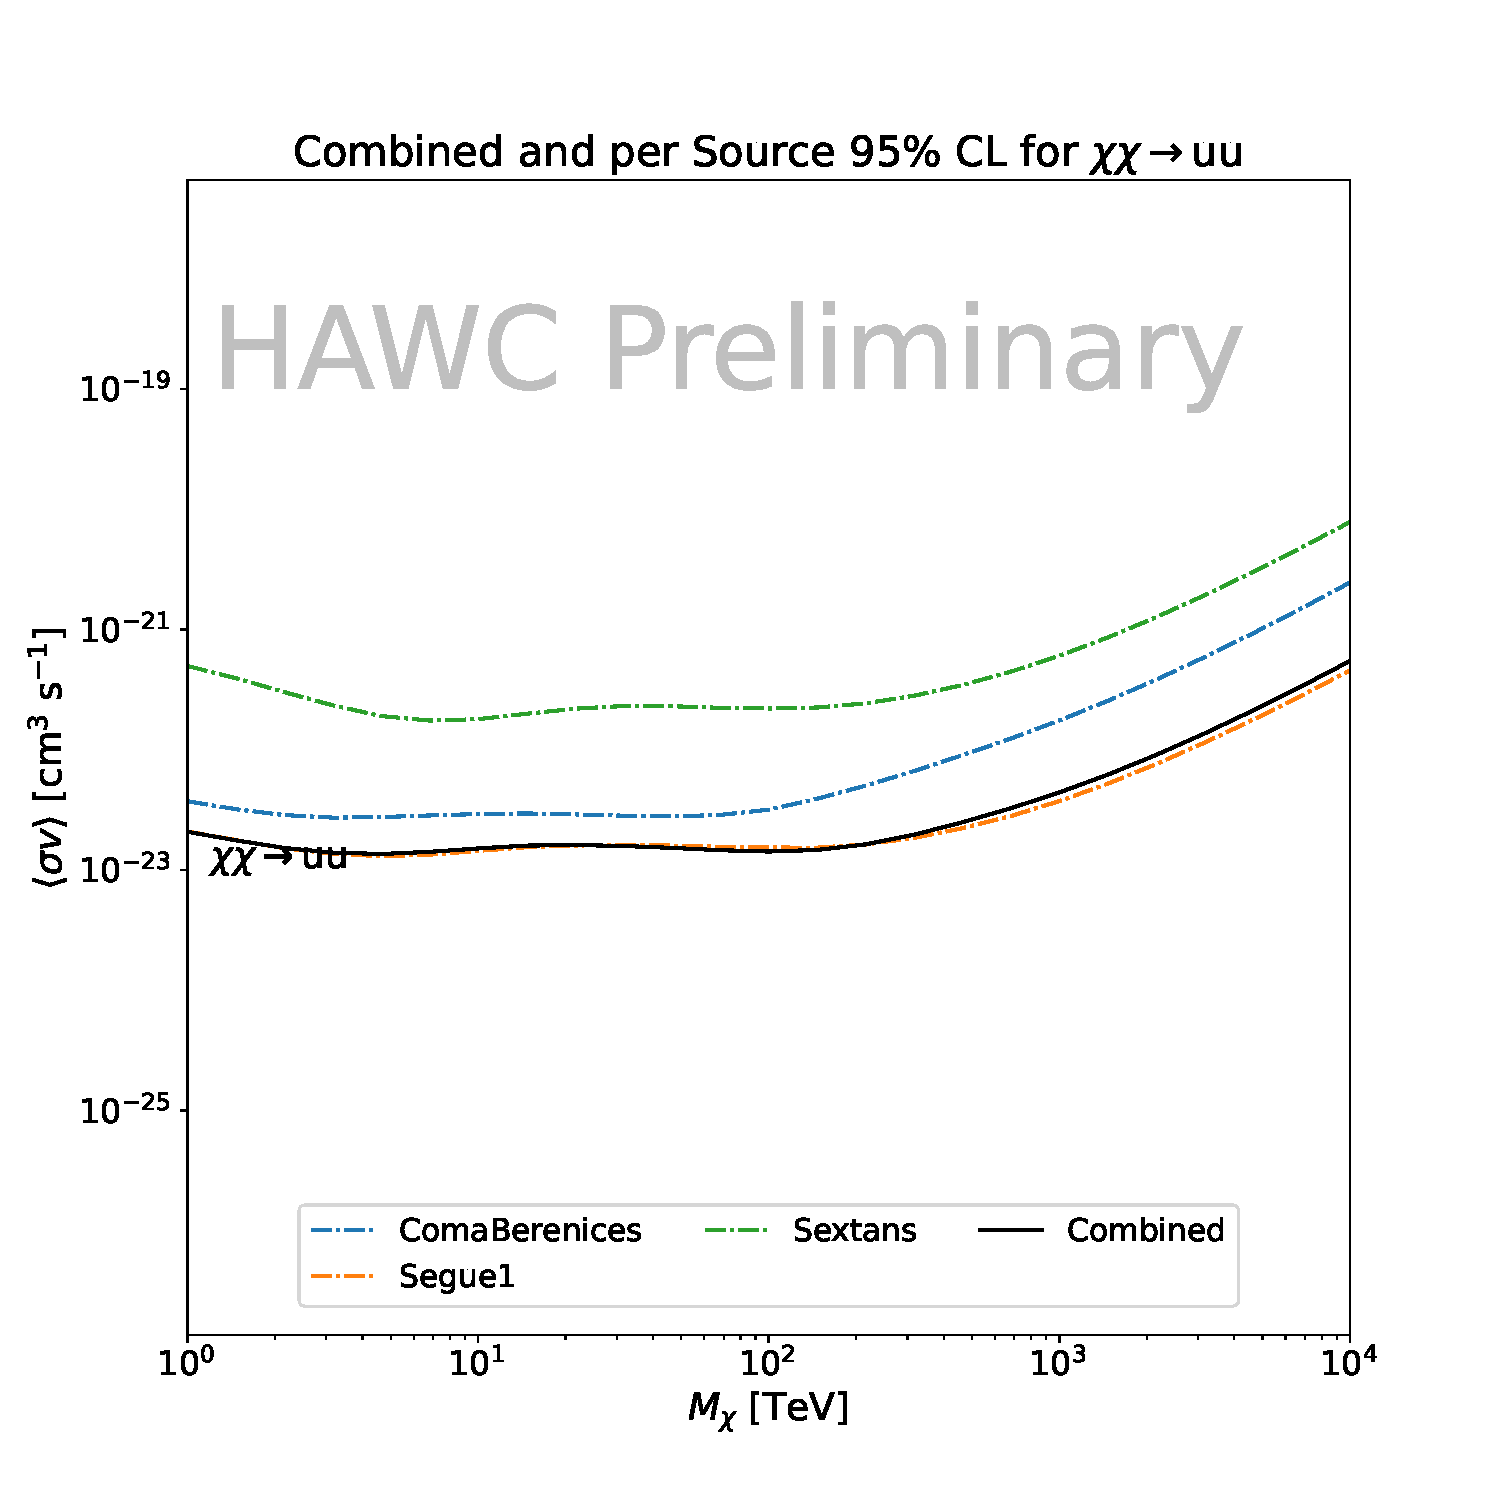
\includegraphics[scale=0.21]{figures/mtd_hawc_dm/results/Combined95_New_duck_uu_.pdf}
    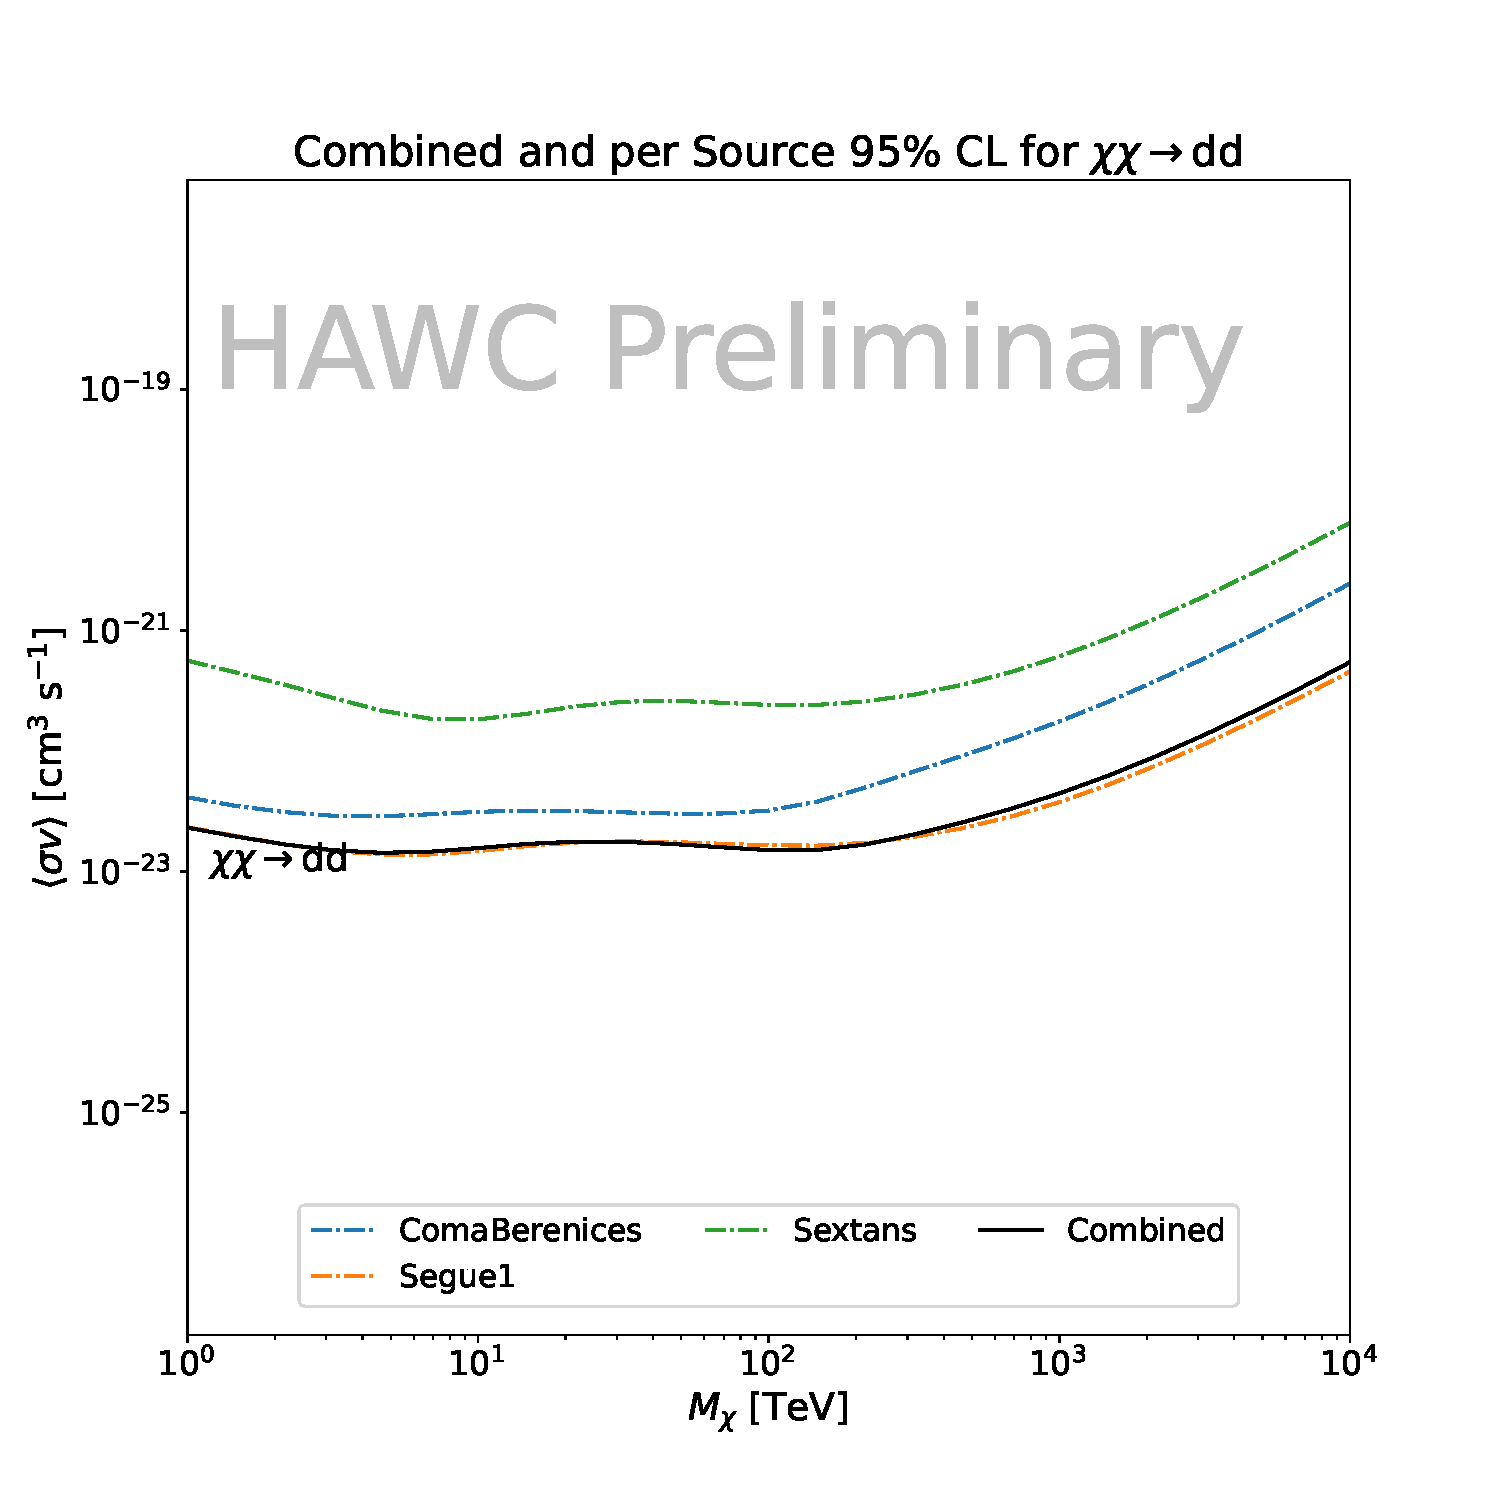
\includegraphics[scale=0.21]{figures/mtd_hawc_dm/results/Combined95_New_duck_dd_.pdf}
    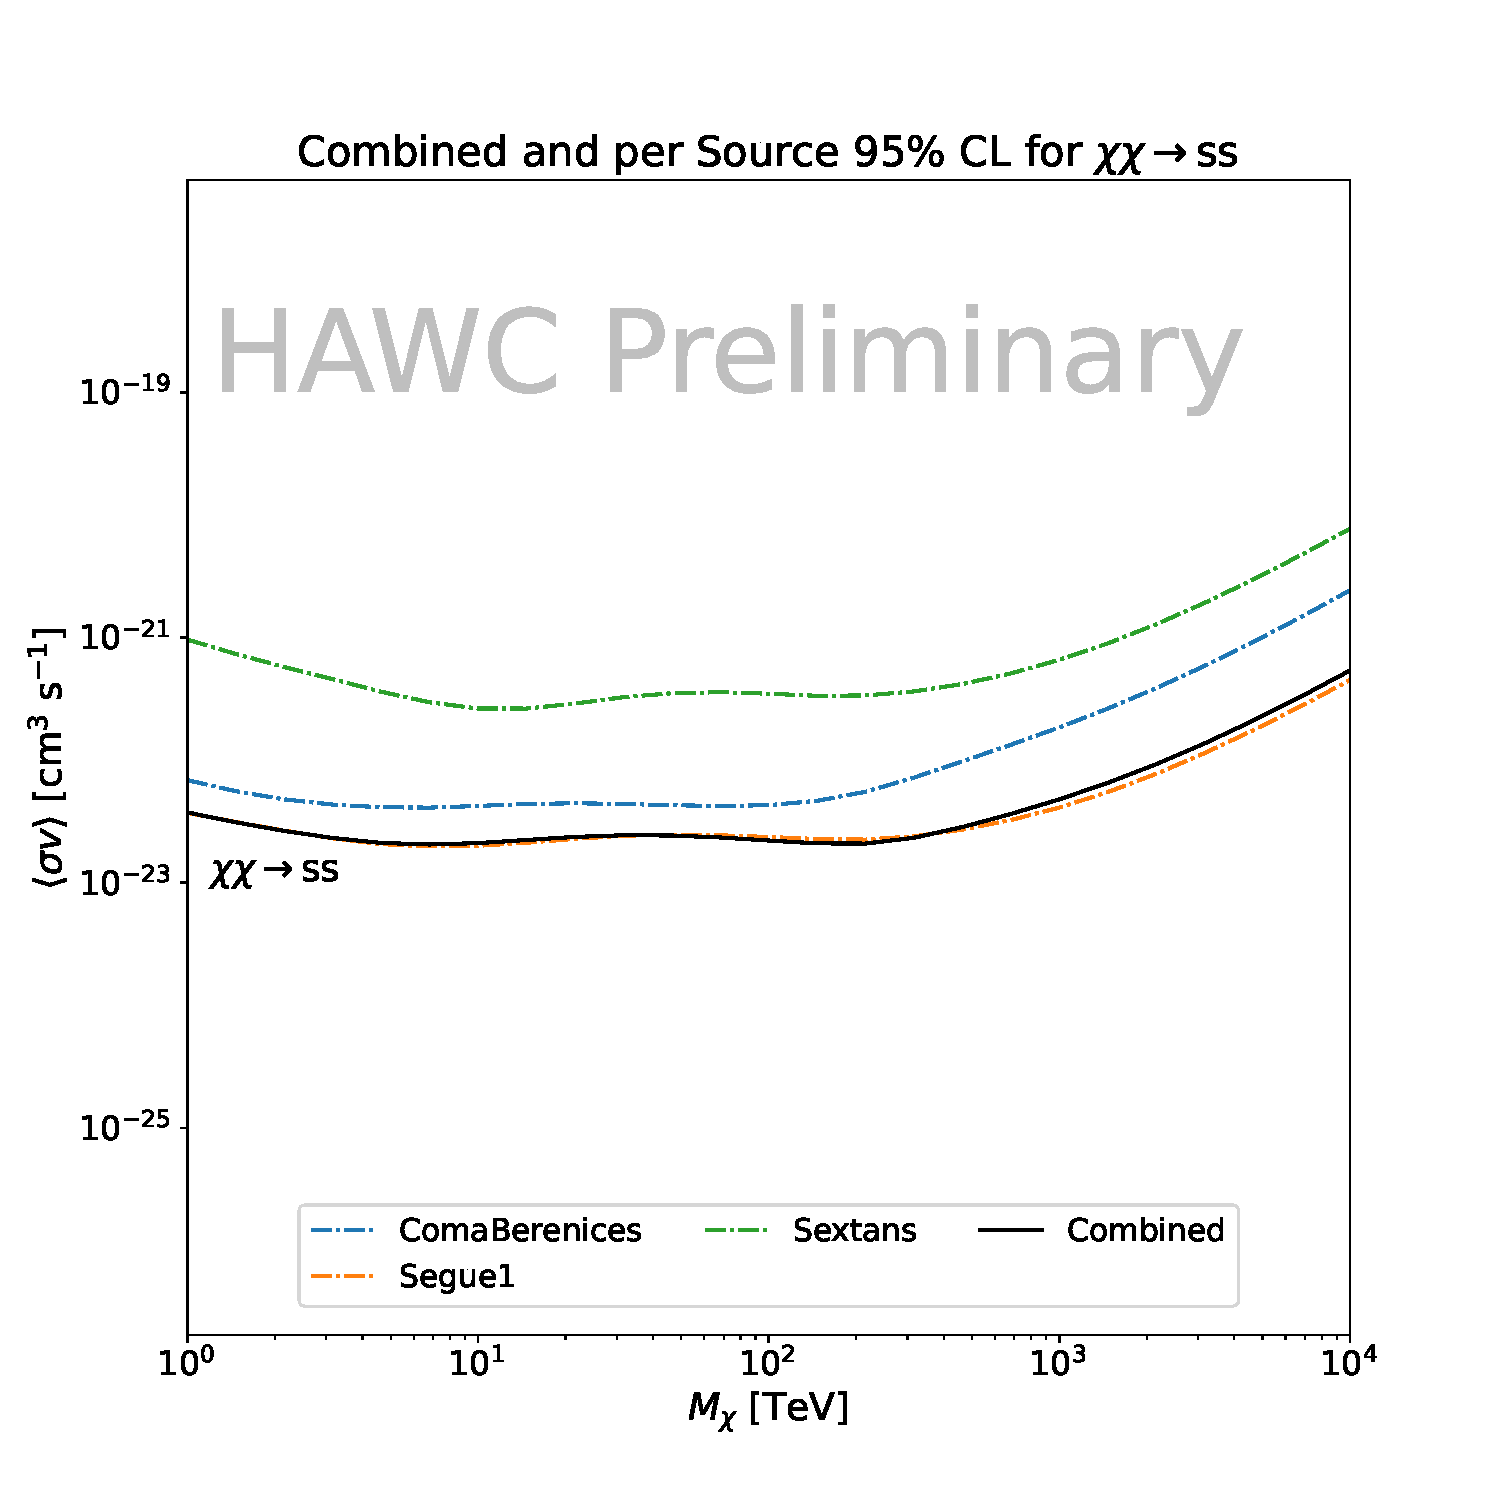
\includegraphics[scale=0.21]{figures/mtd_hawc_dm/results/Combined95_New_duck_ss_.pdf}
    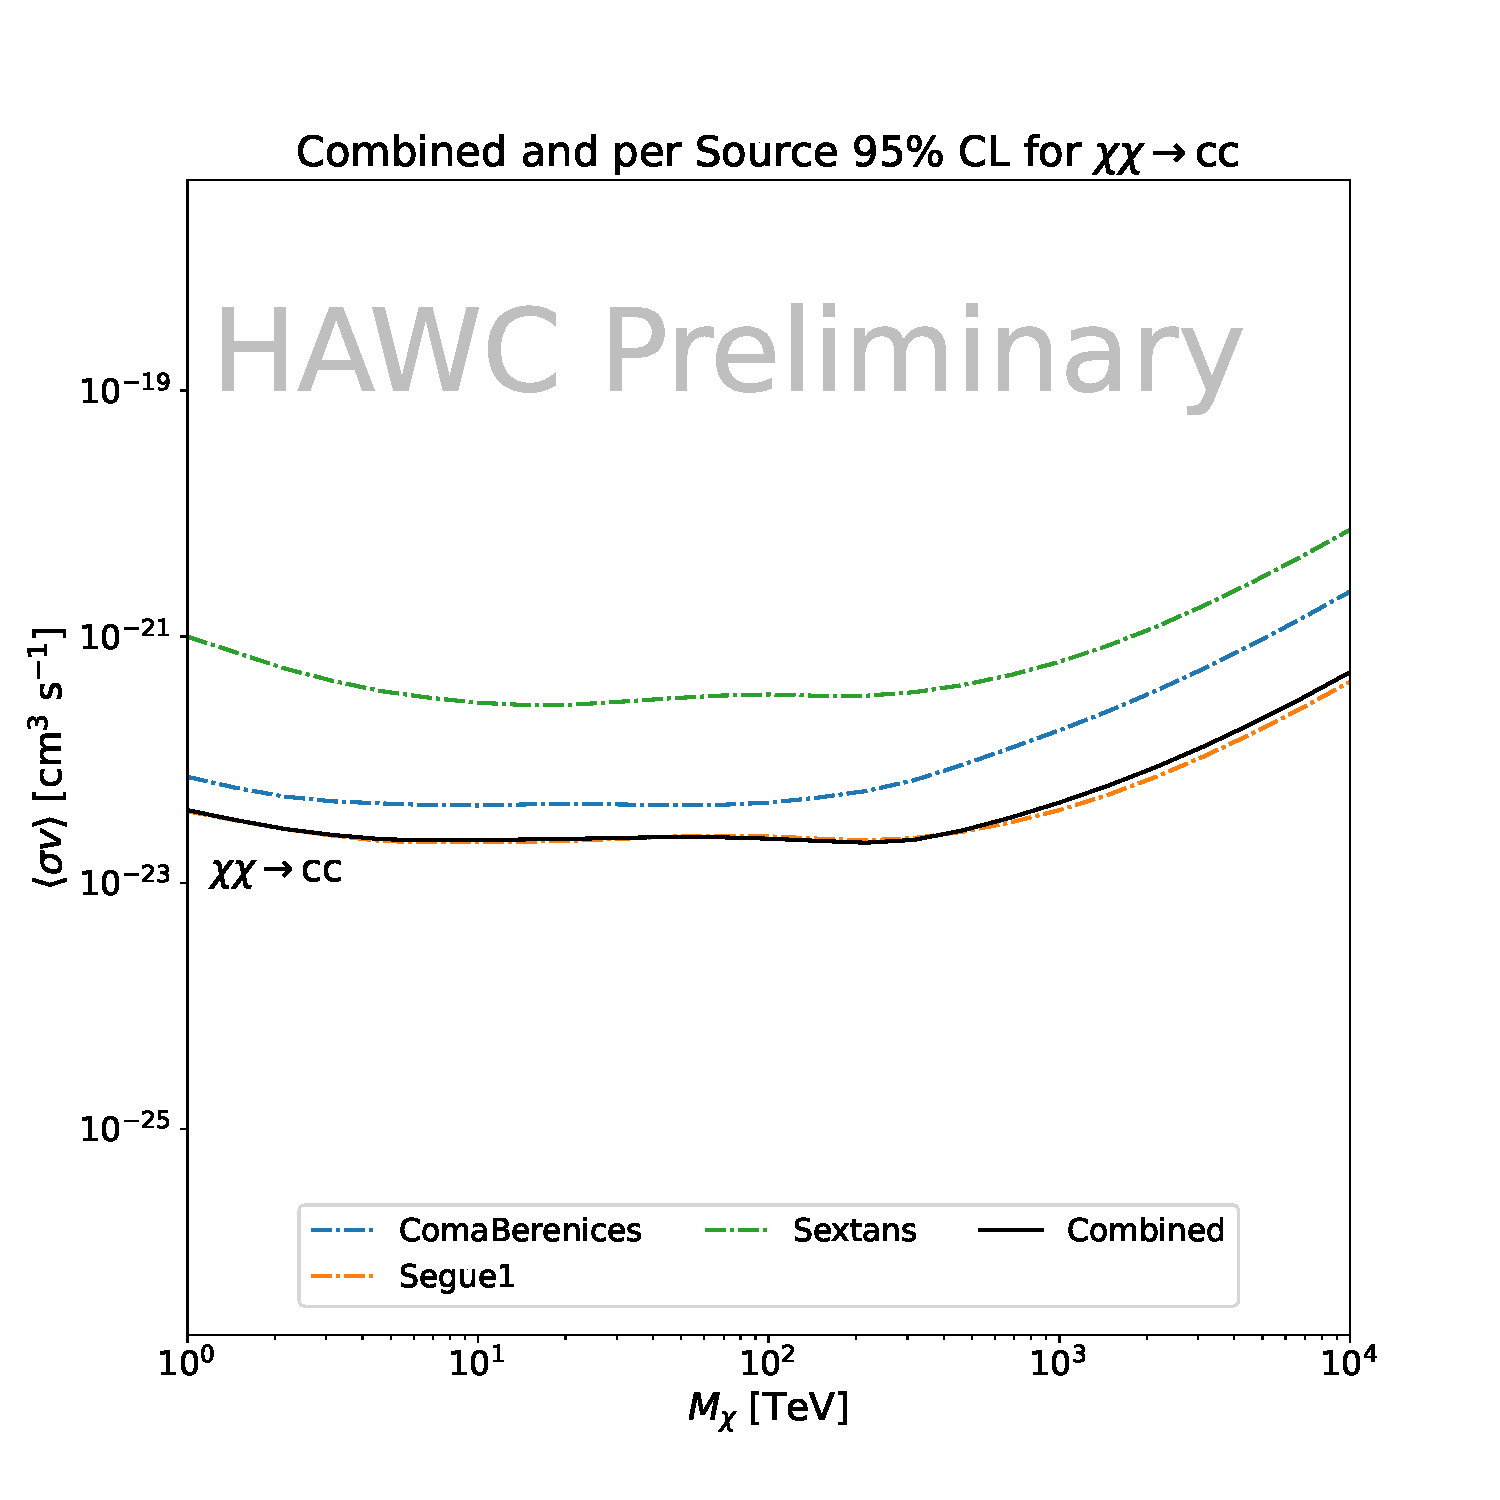
\includegraphics[scale=0.21]{figures/mtd_hawc_dm/results/Combined95_New_duck_cc_.pdf}
    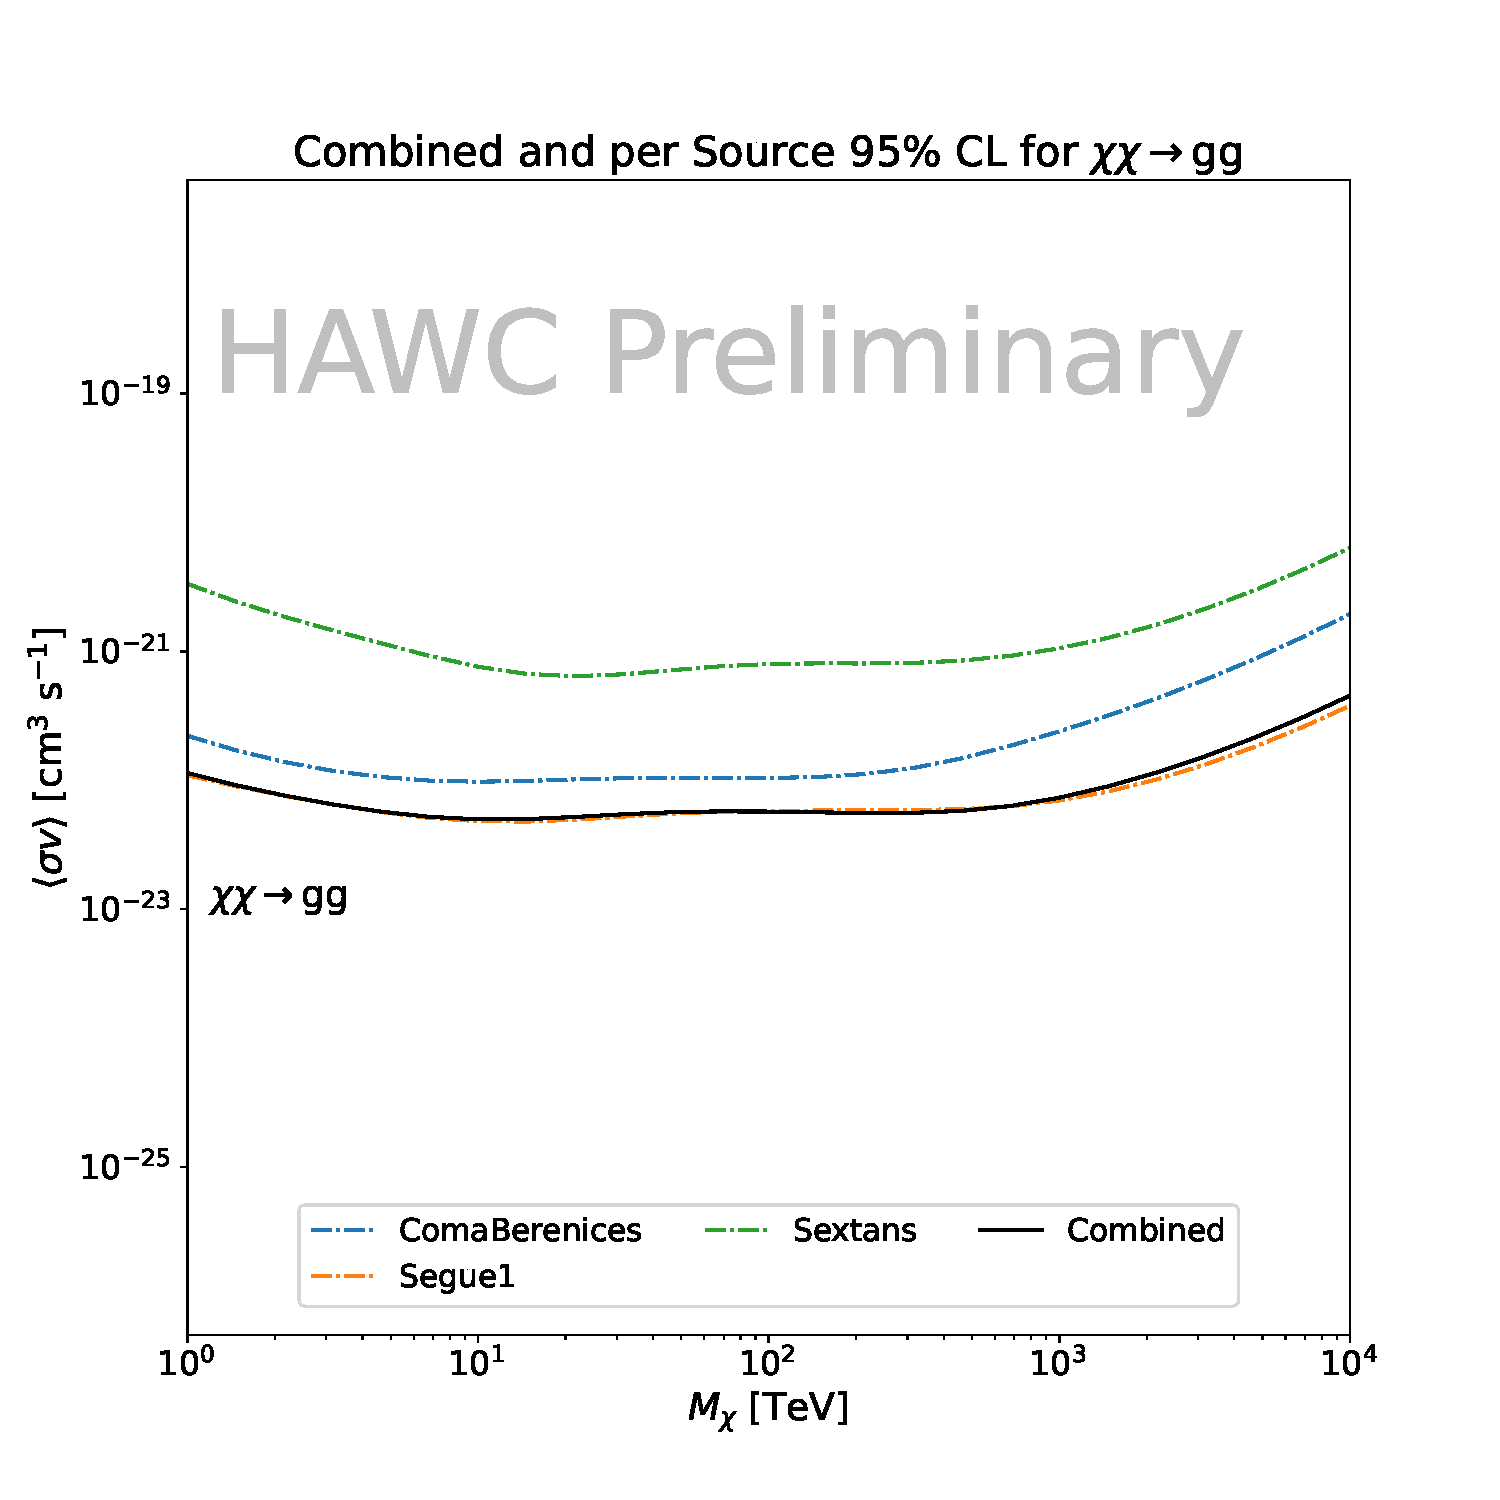
\includegraphics[scale=0.21]{figures/mtd_hawc_dm/results/Combined95_New_duck_gg_.pdf}
    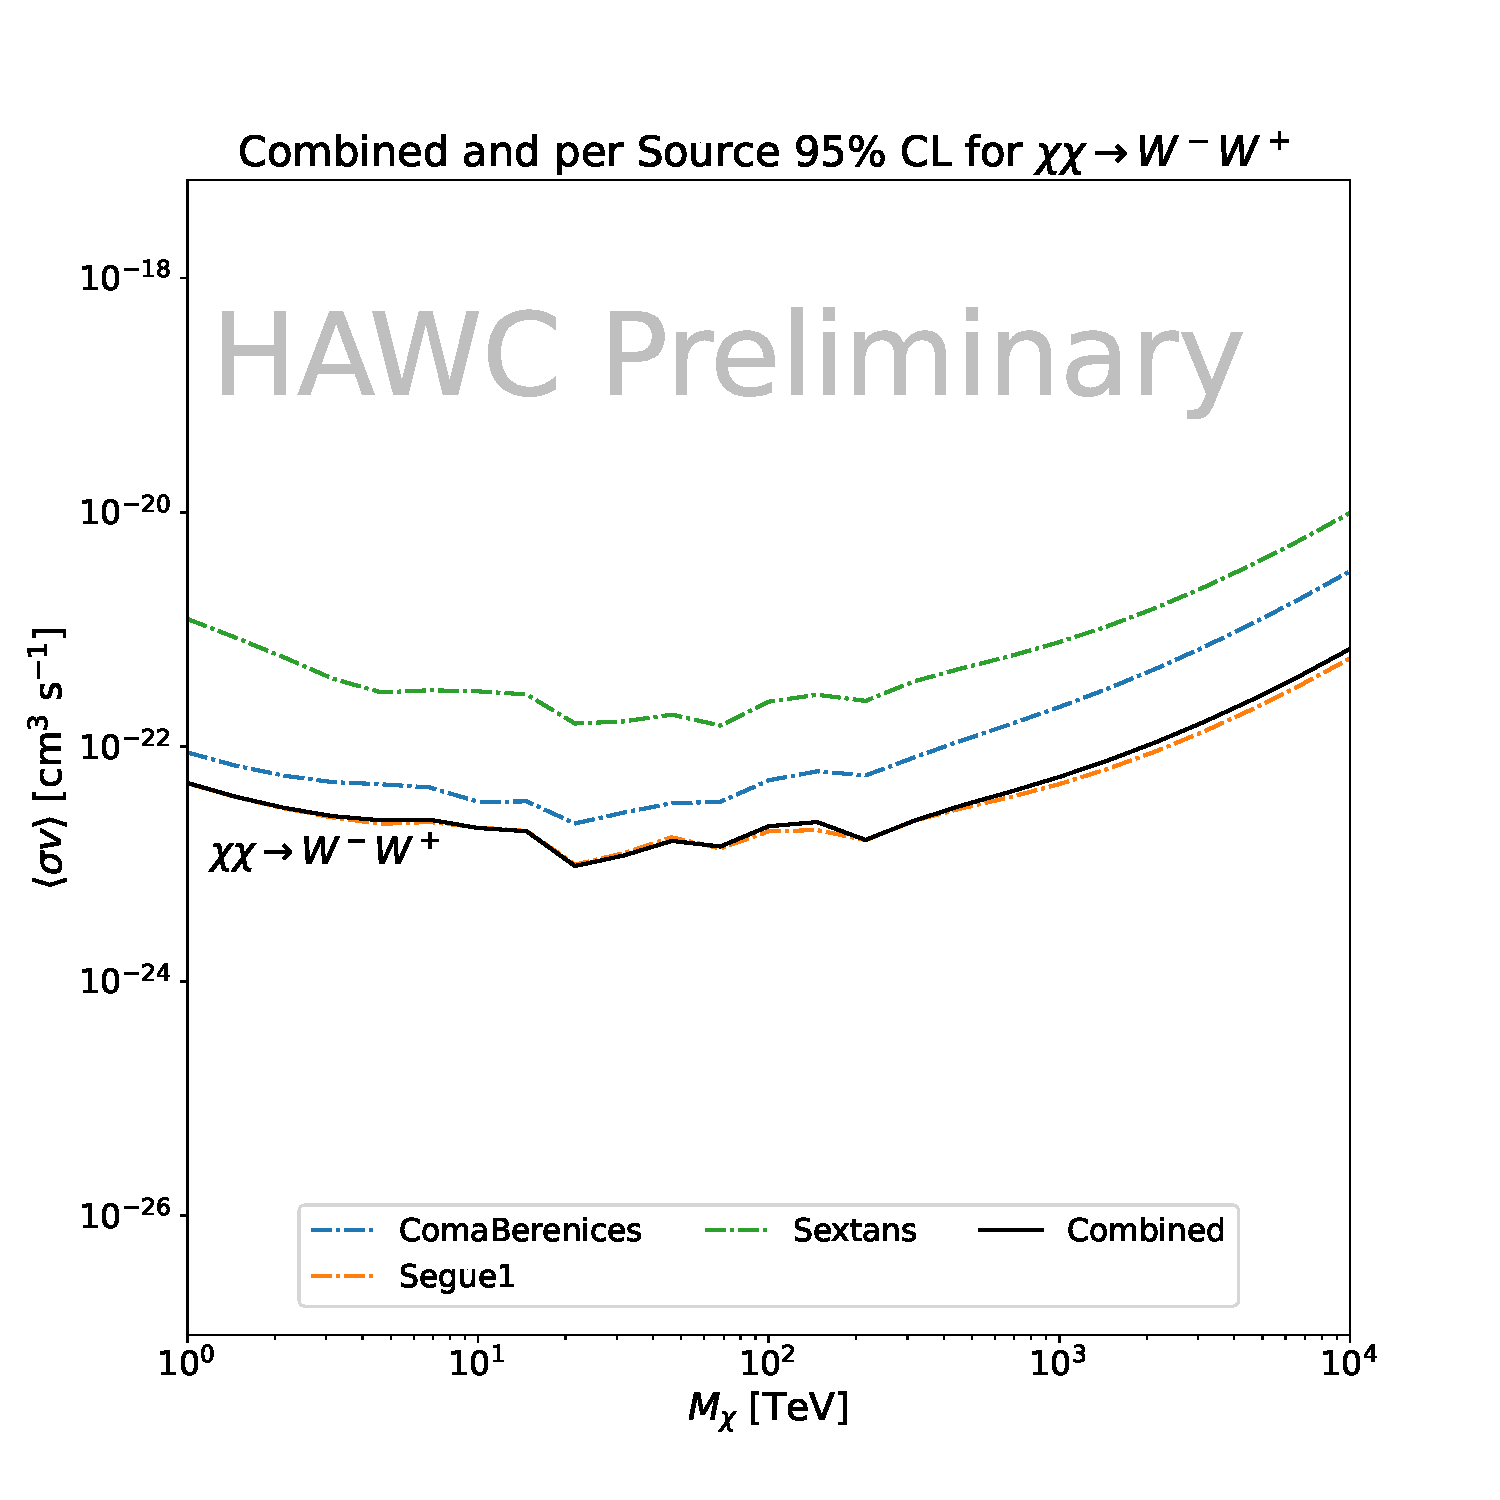
\includegraphics[scale=0.21]{figures/mtd_hawc_dm/results/Combined95_New_duck_ww_.pdf}
    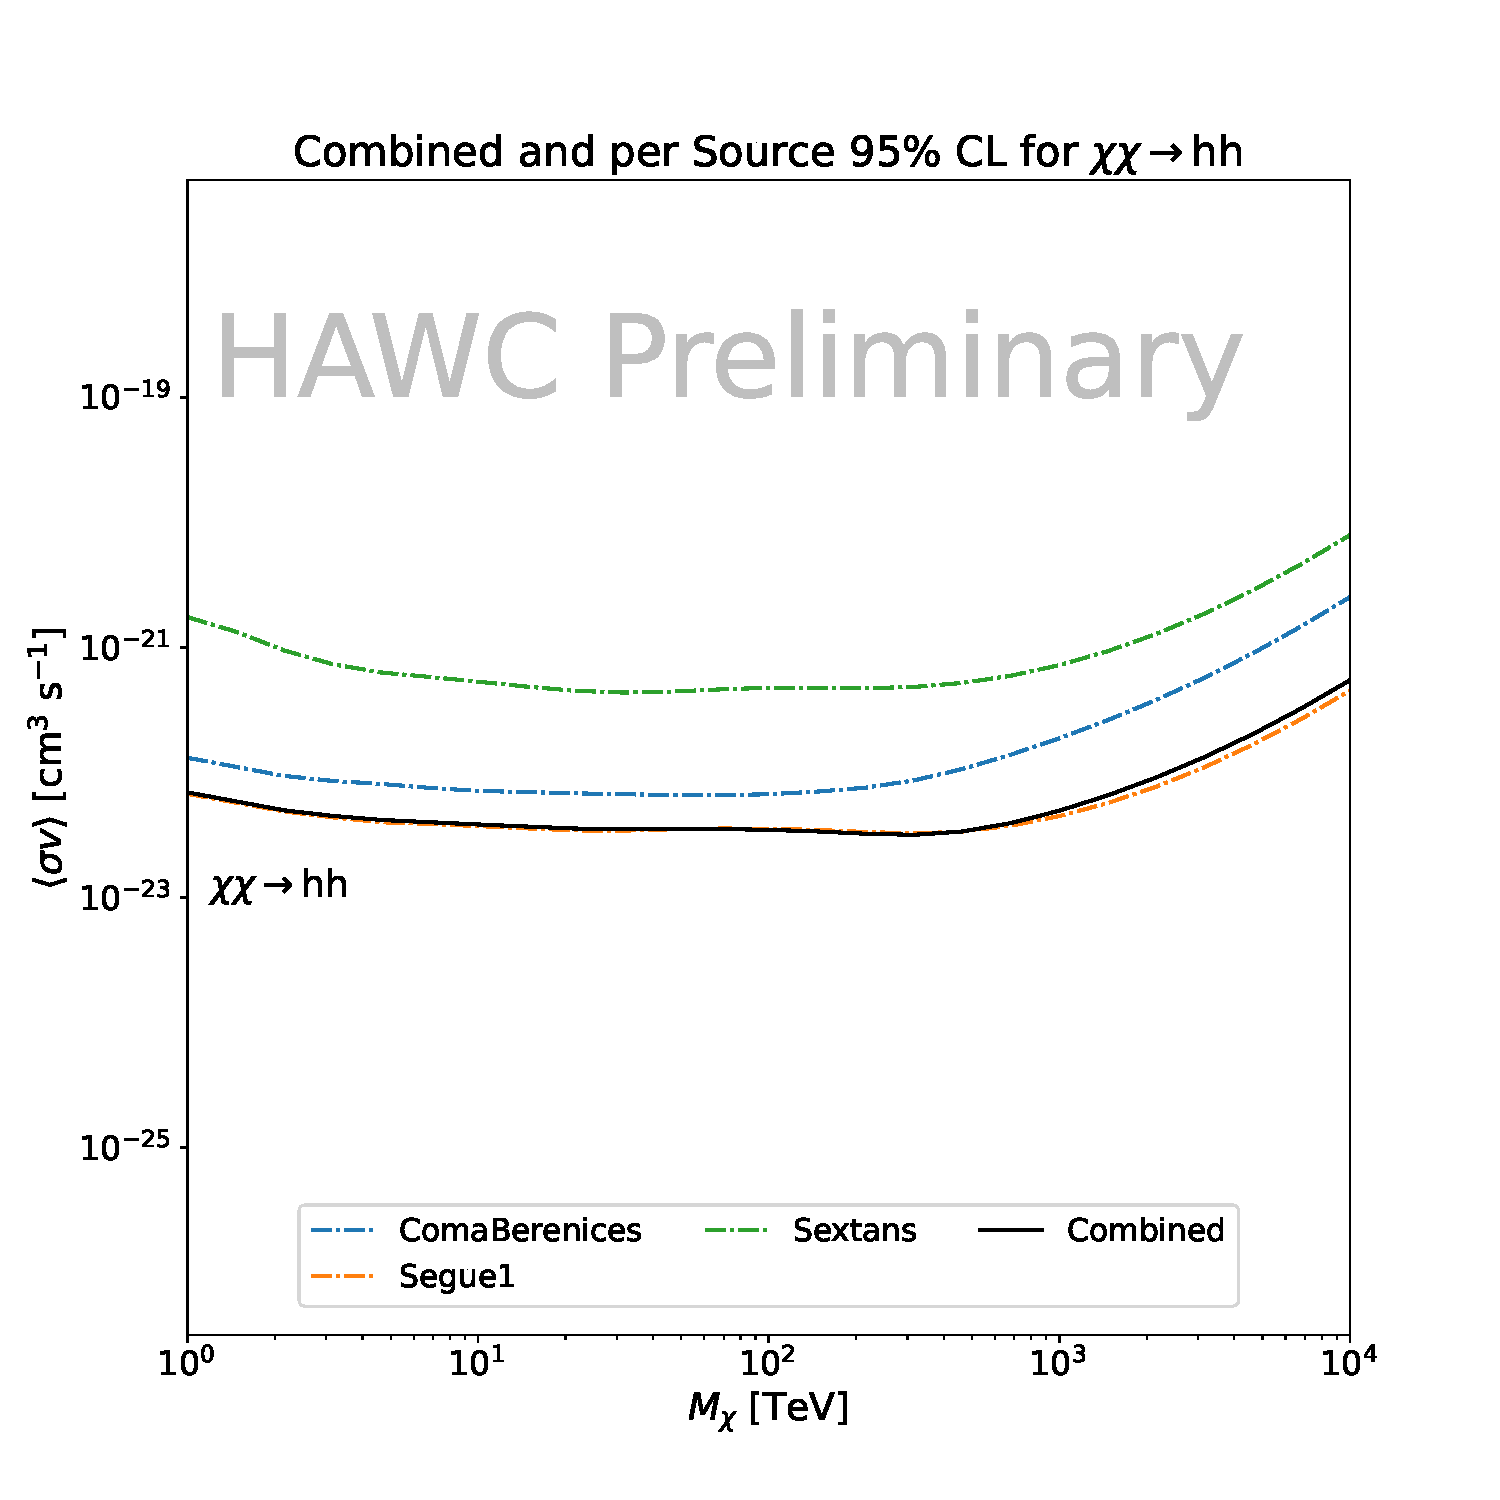
\includegraphics[scale=0.21]{figures/mtd_hawc_dm/results/Combined95_New_duck_hh_.pdf}
    }
    \caption{HAWC upper limits at 95\% confidence level on \sv~versus $m_\chi$ for $\chi\chi \rightarrow $ \parpar{b}, \parpar{t}, \parpar{u}, \parpar{d}, \parpar{s}, \parpar{c}, \pp{g}, $W^+ W^-$, and \pp{h}. Limits are with \LS \J-factors \cite{DM_Strigari20}. The solid line represents the observed combined limit. Dashed lines represent limits from individual dSphs.}
\label{fig:mtd_limits_1of2}
\end{figure}

\begin{figure}[h]
\centering{
    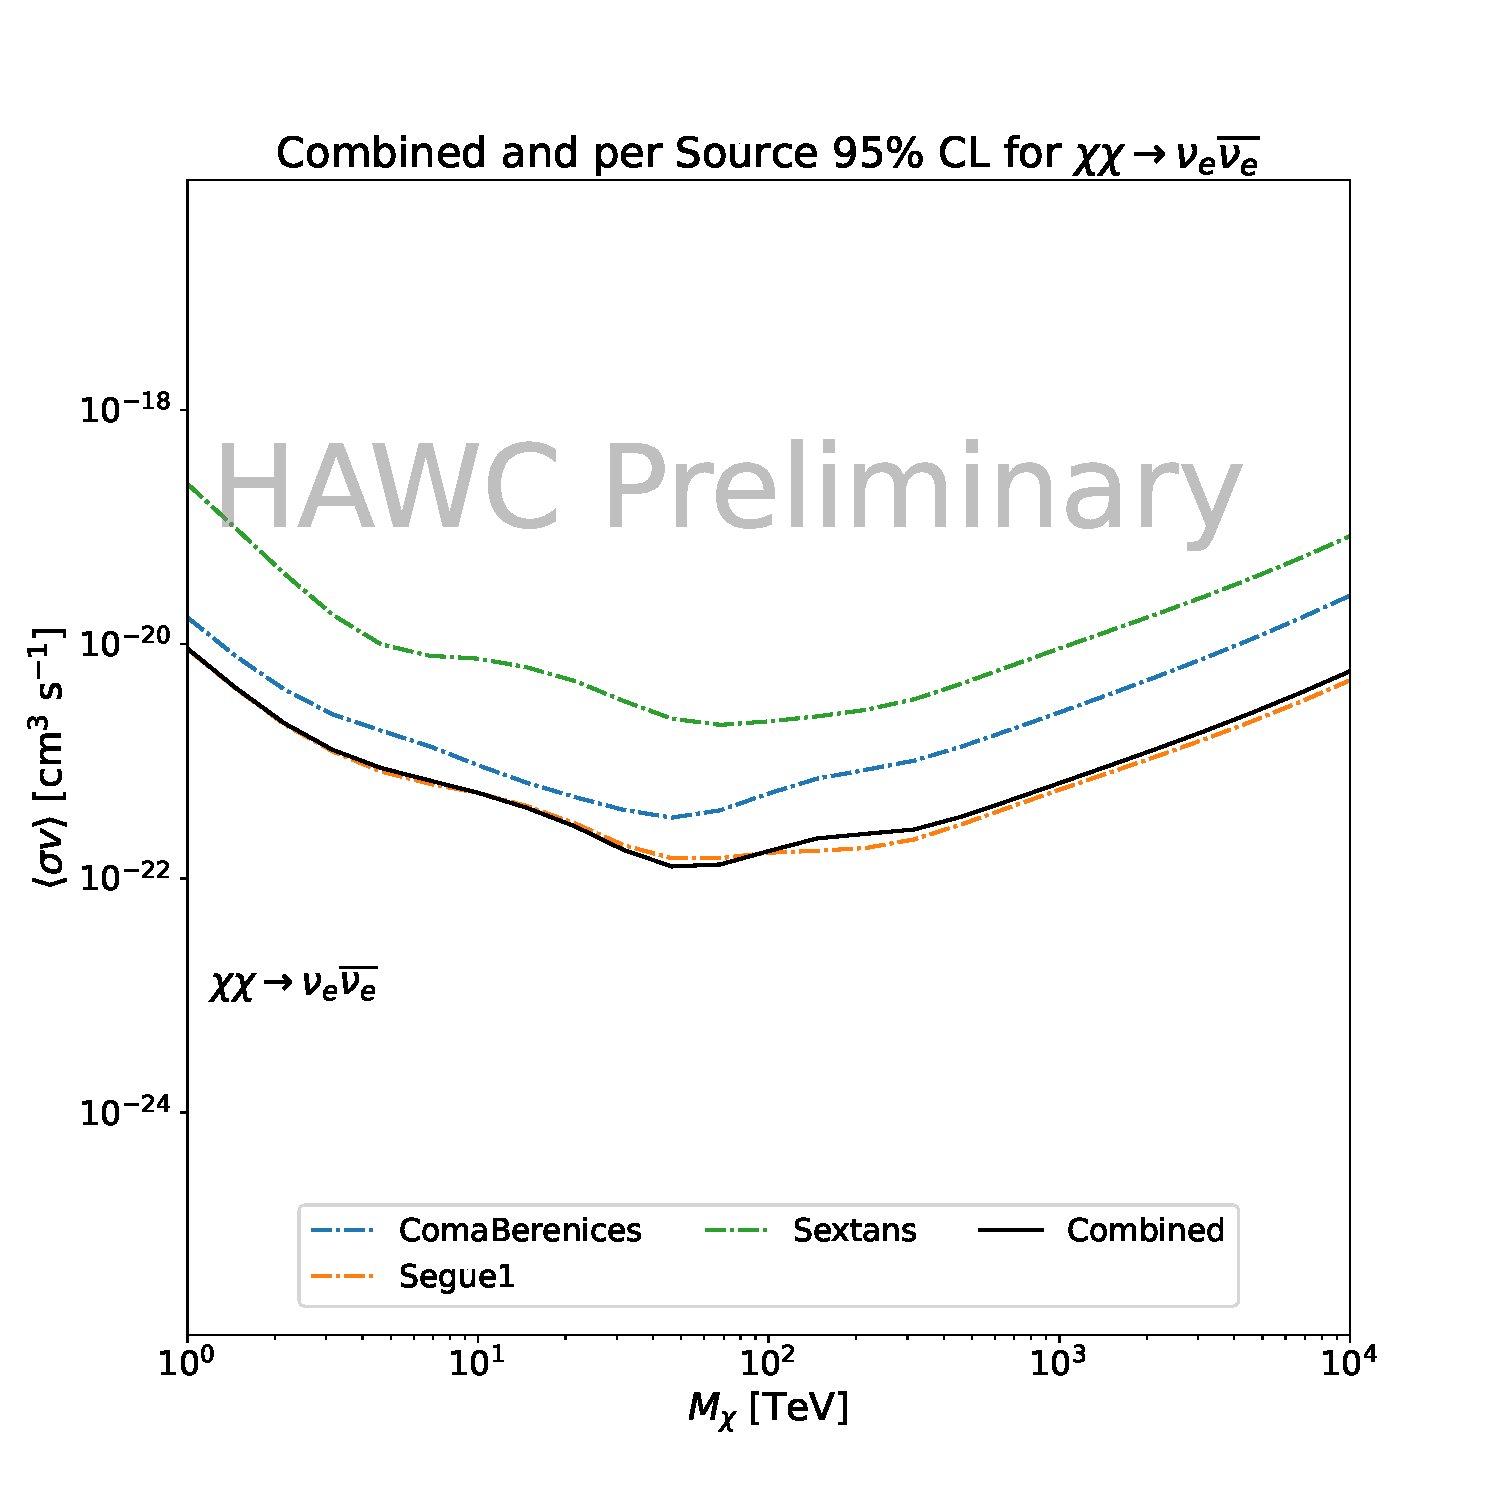
\includegraphics[scale=0.21]{figures/mtd_hawc_dm/results/Combined95_New_duck_nuenue_.pdf}
    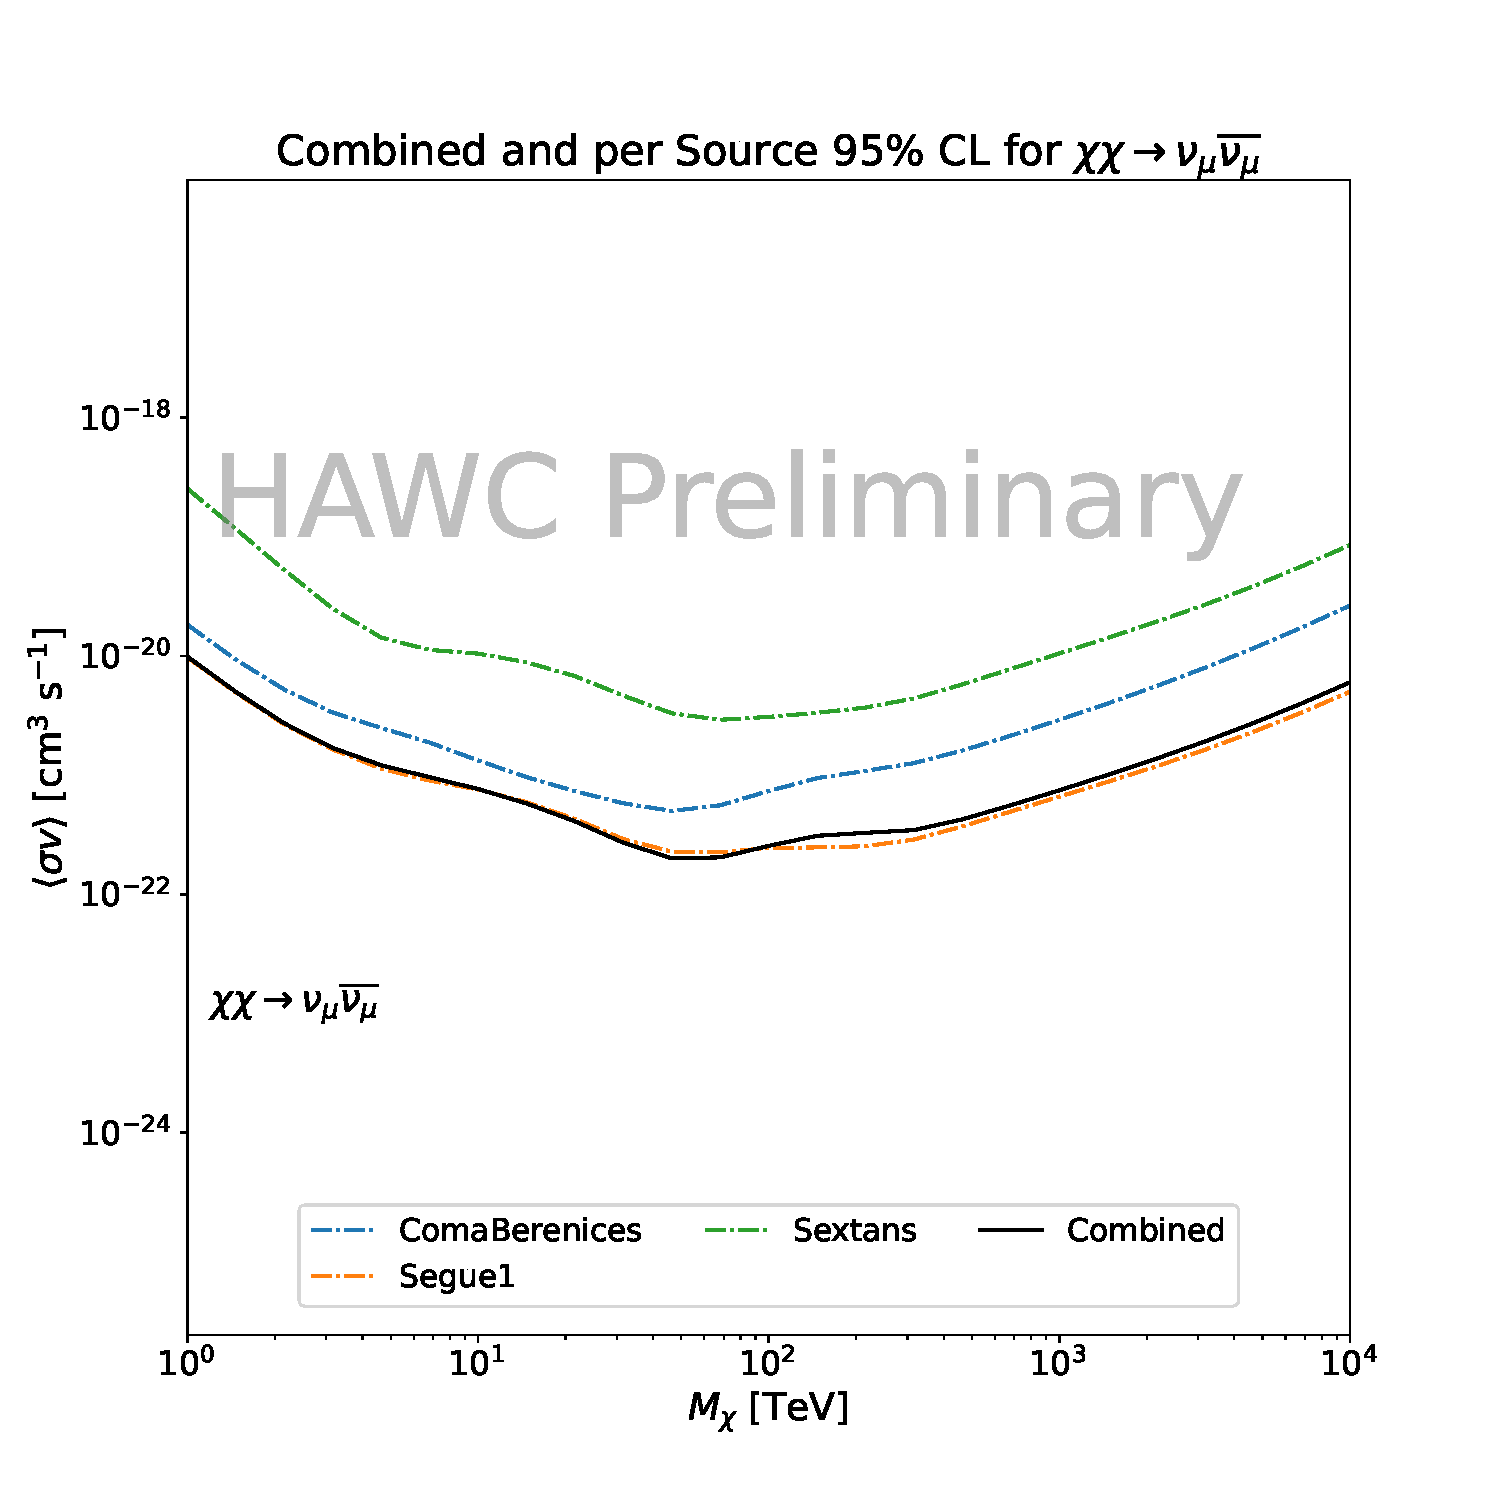
\includegraphics[scale=0.21]{figures/mtd_hawc_dm/results/Combined95_New_duck_numunumu_.pdf}
    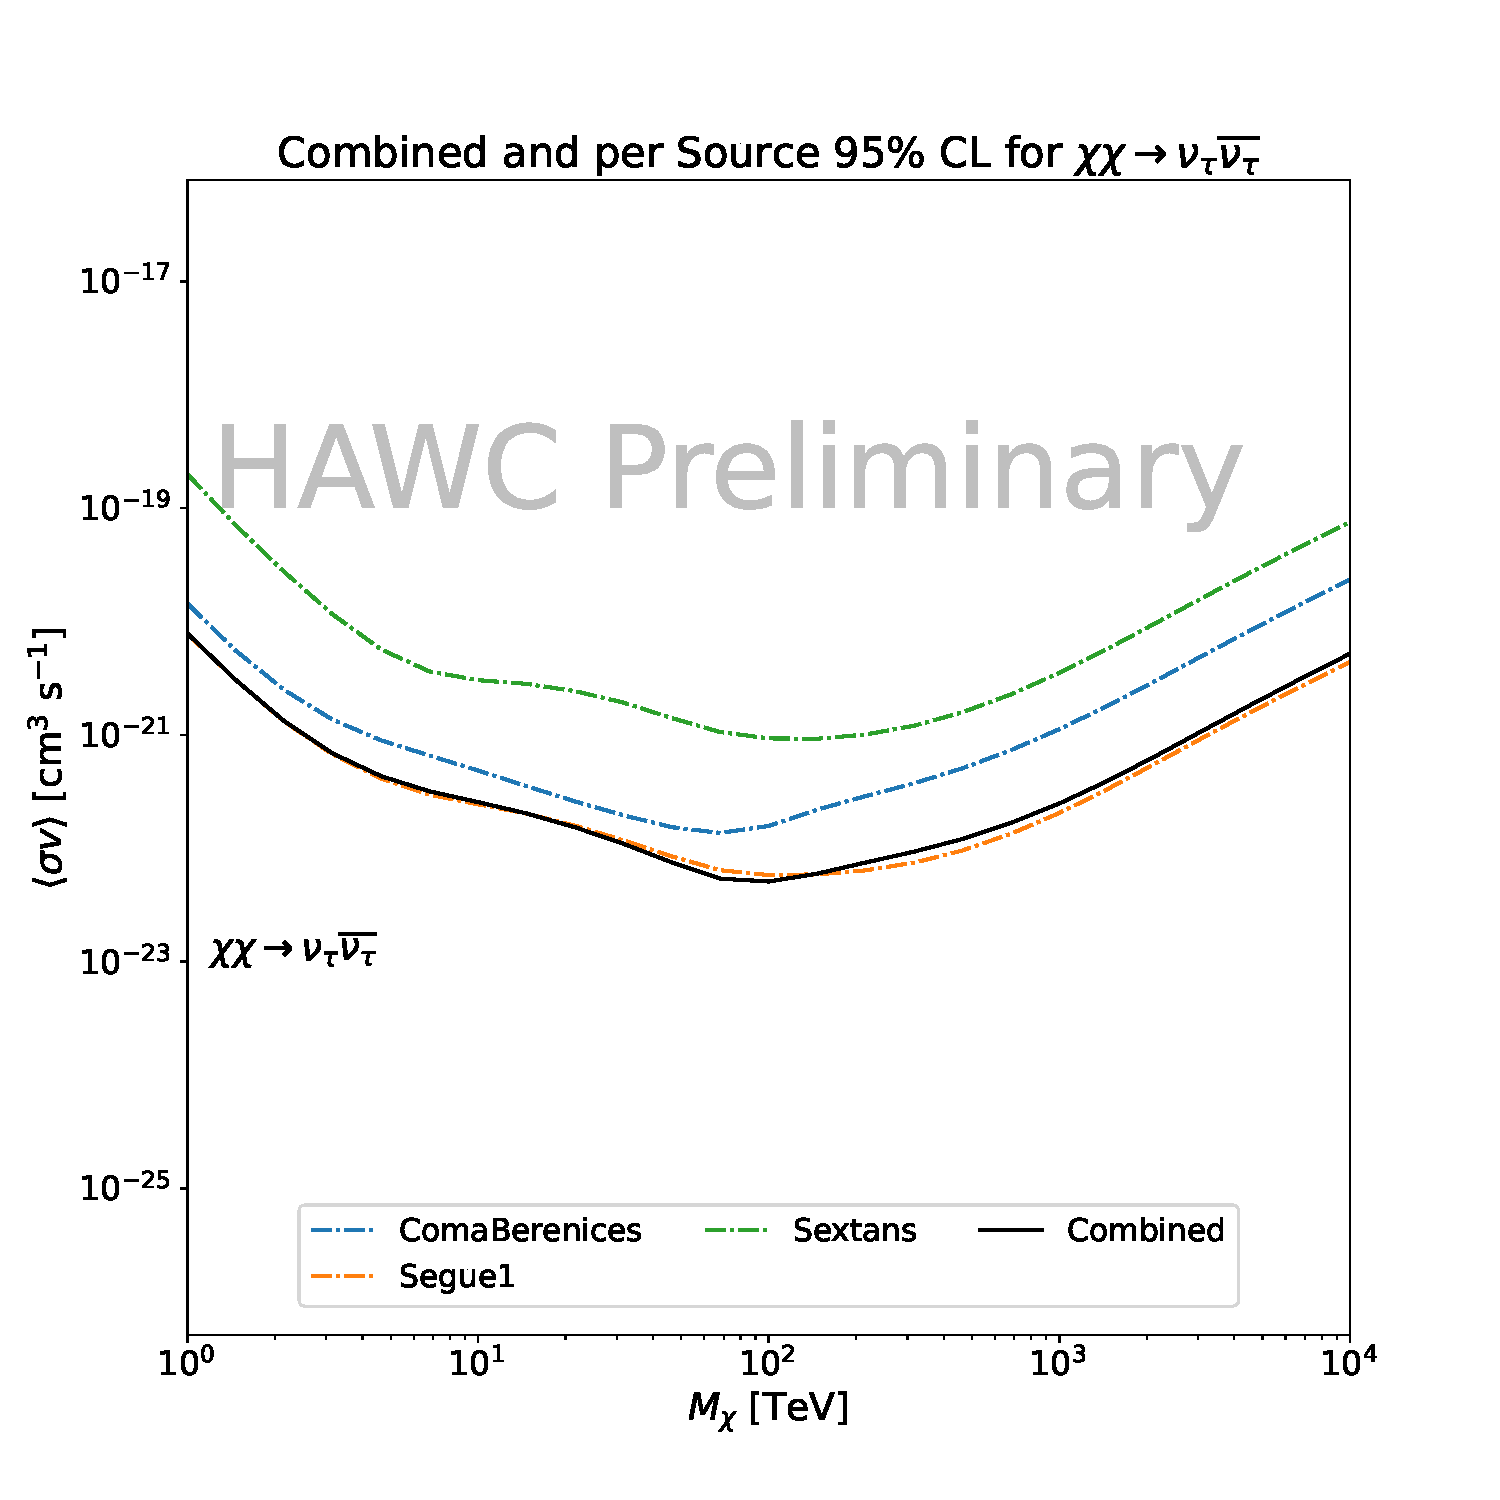
\includegraphics[scale=0.21]{figures/mtd_hawc_dm/results/Combined95_New_duck_nutaunutau_.pdf}
    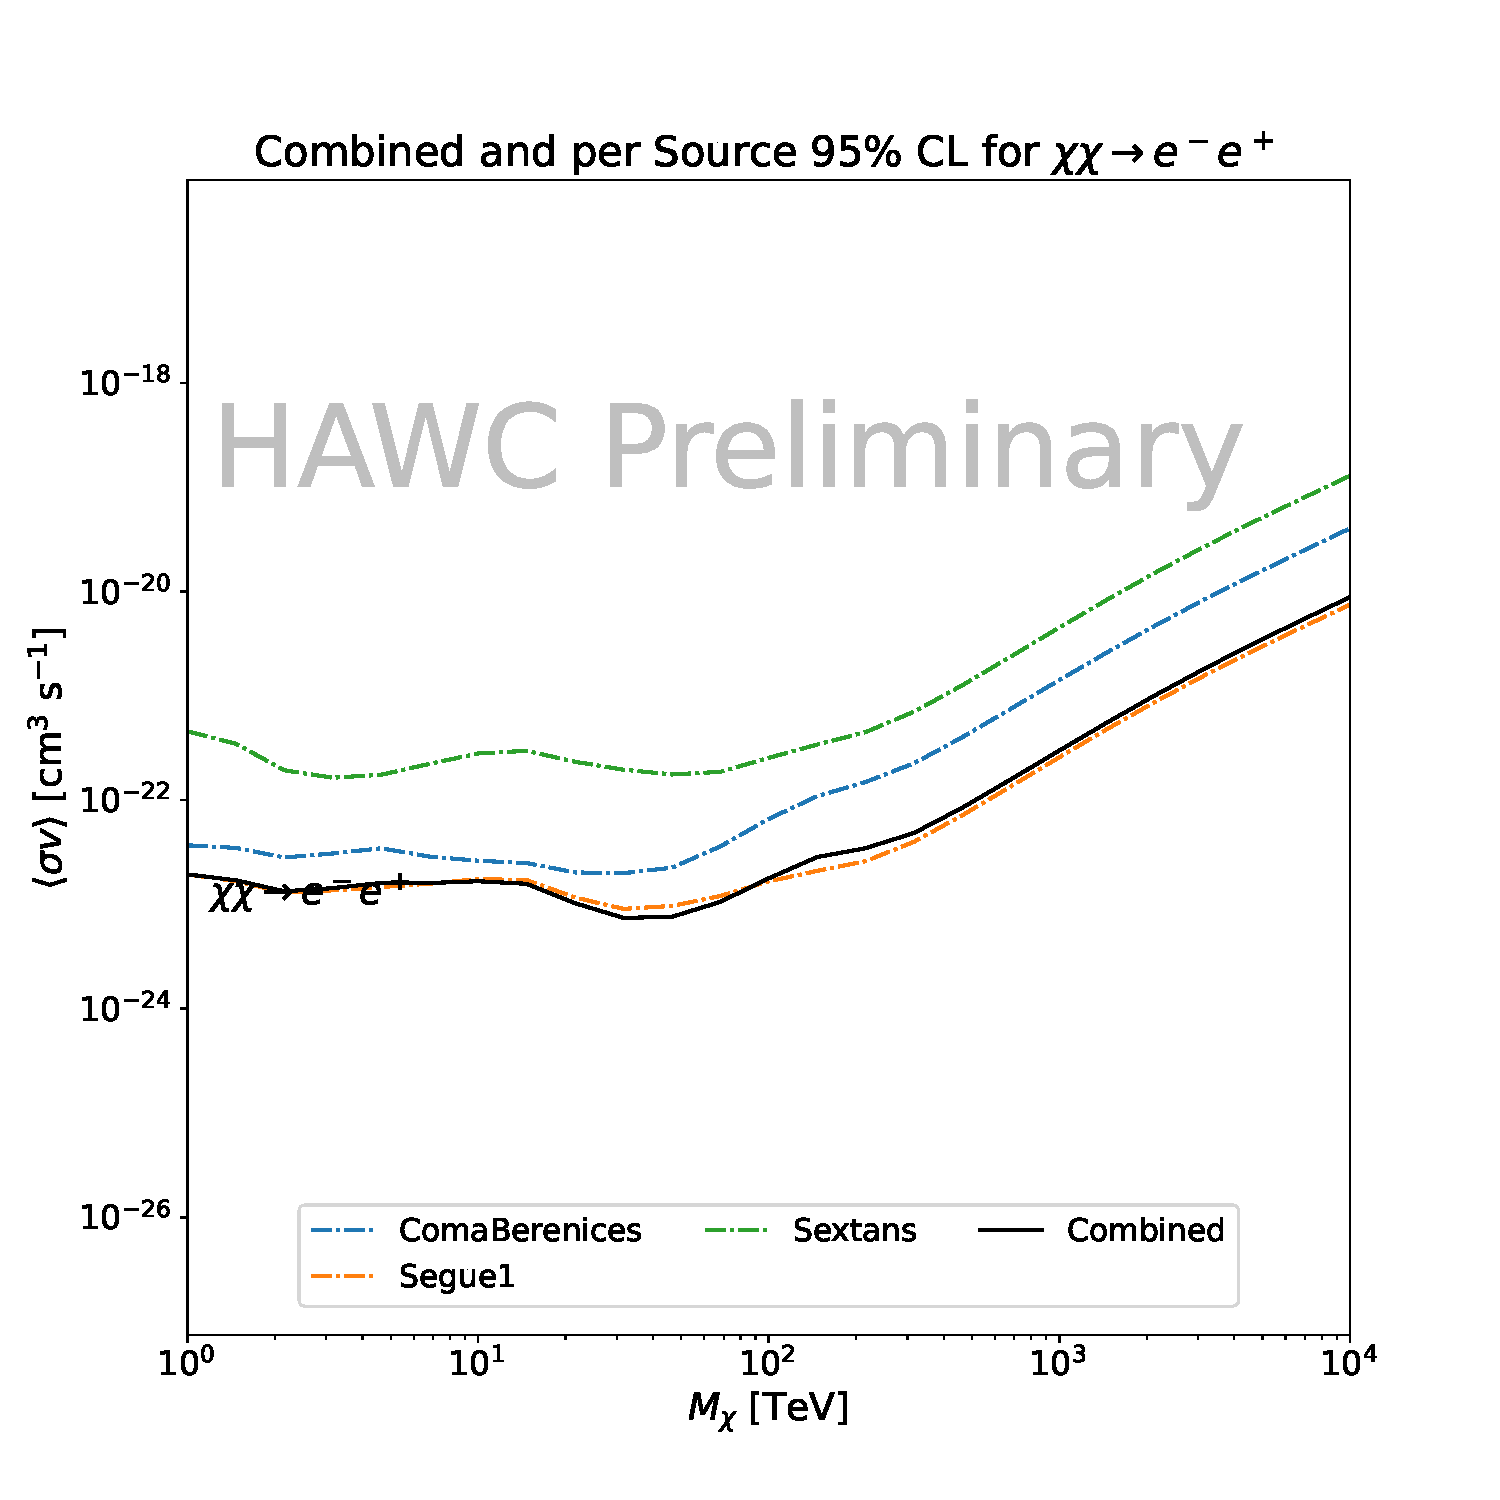
\includegraphics[scale=0.21]{figures/mtd_hawc_dm/results/Combined95_New_duck_ee_.pdf}
    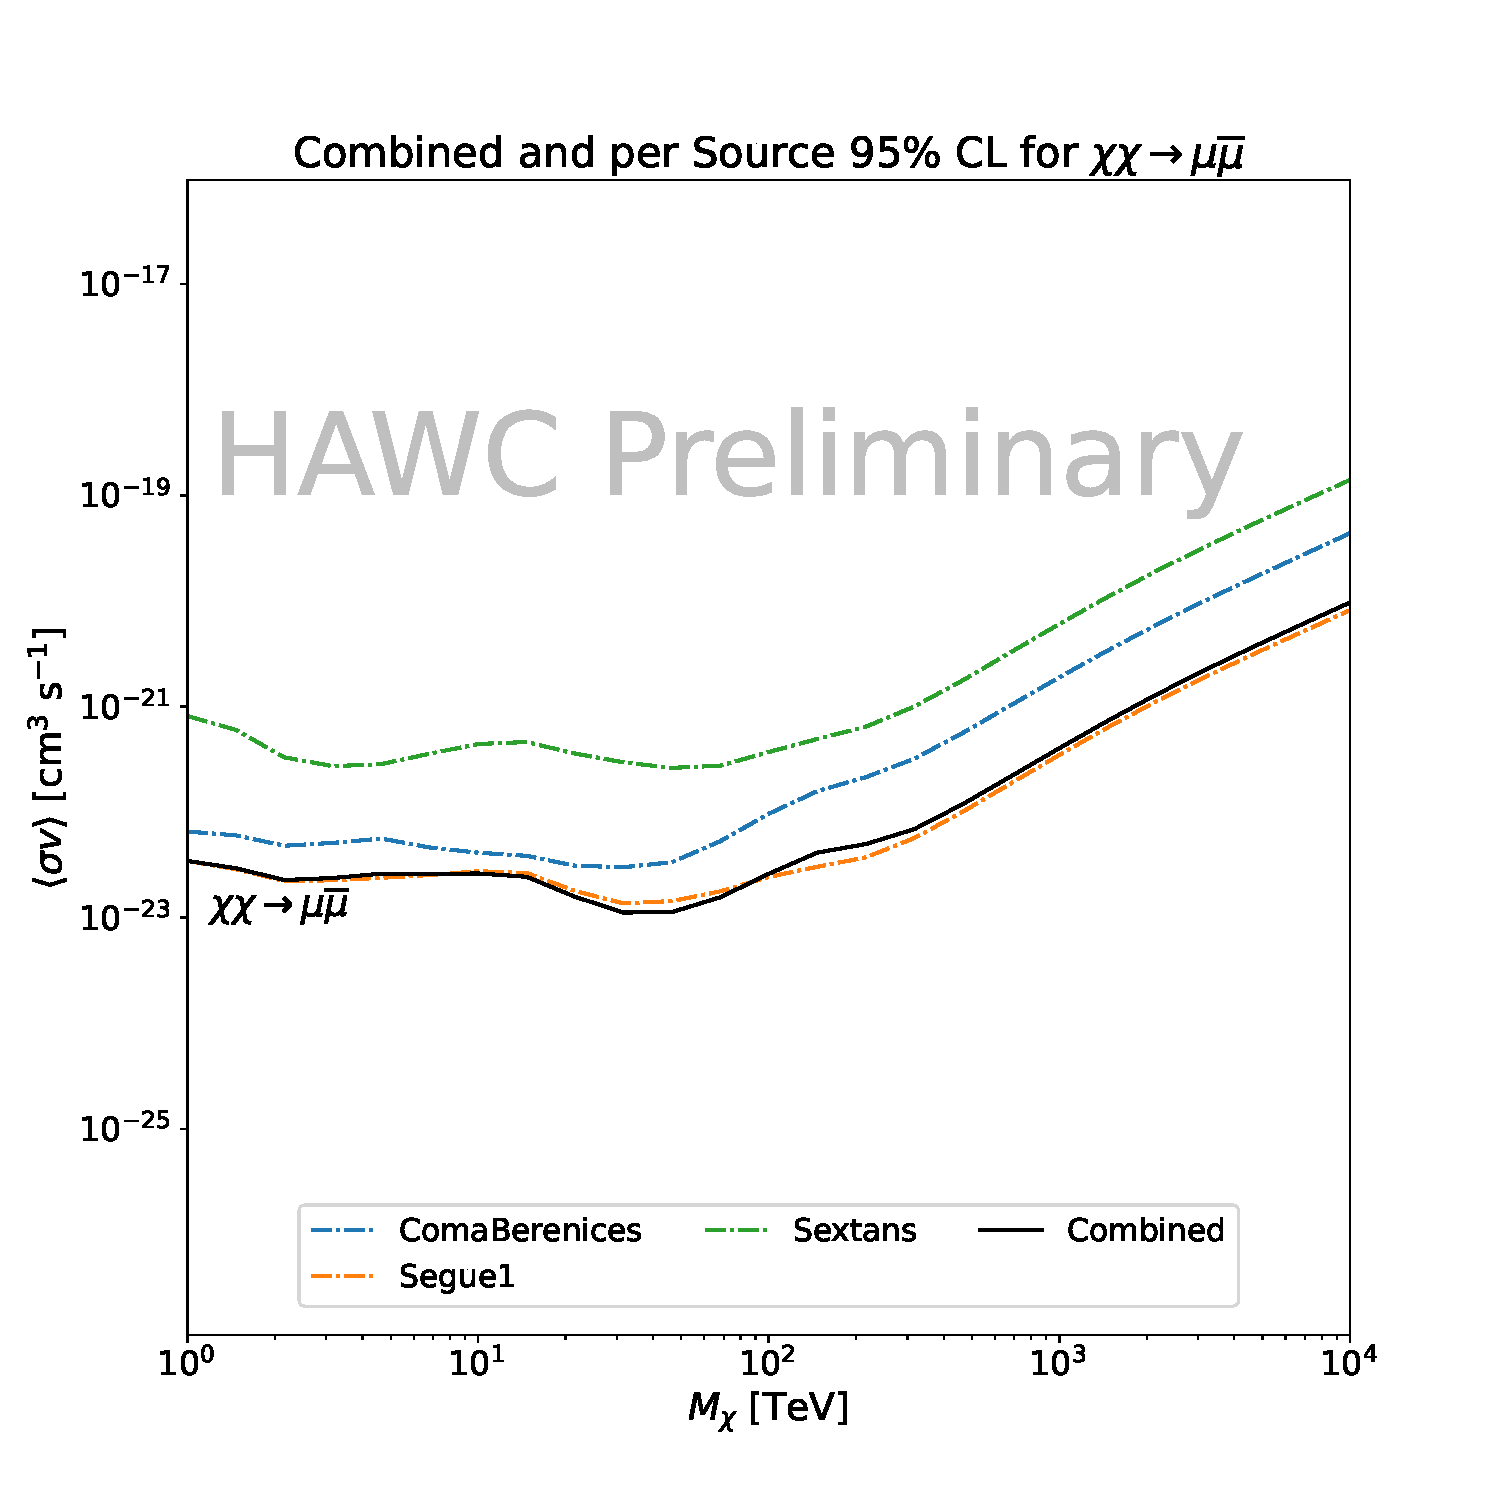
\includegraphics[scale=0.21]{figures/mtd_hawc_dm/results/Combined95_New_duck_mumu_.pdf}
    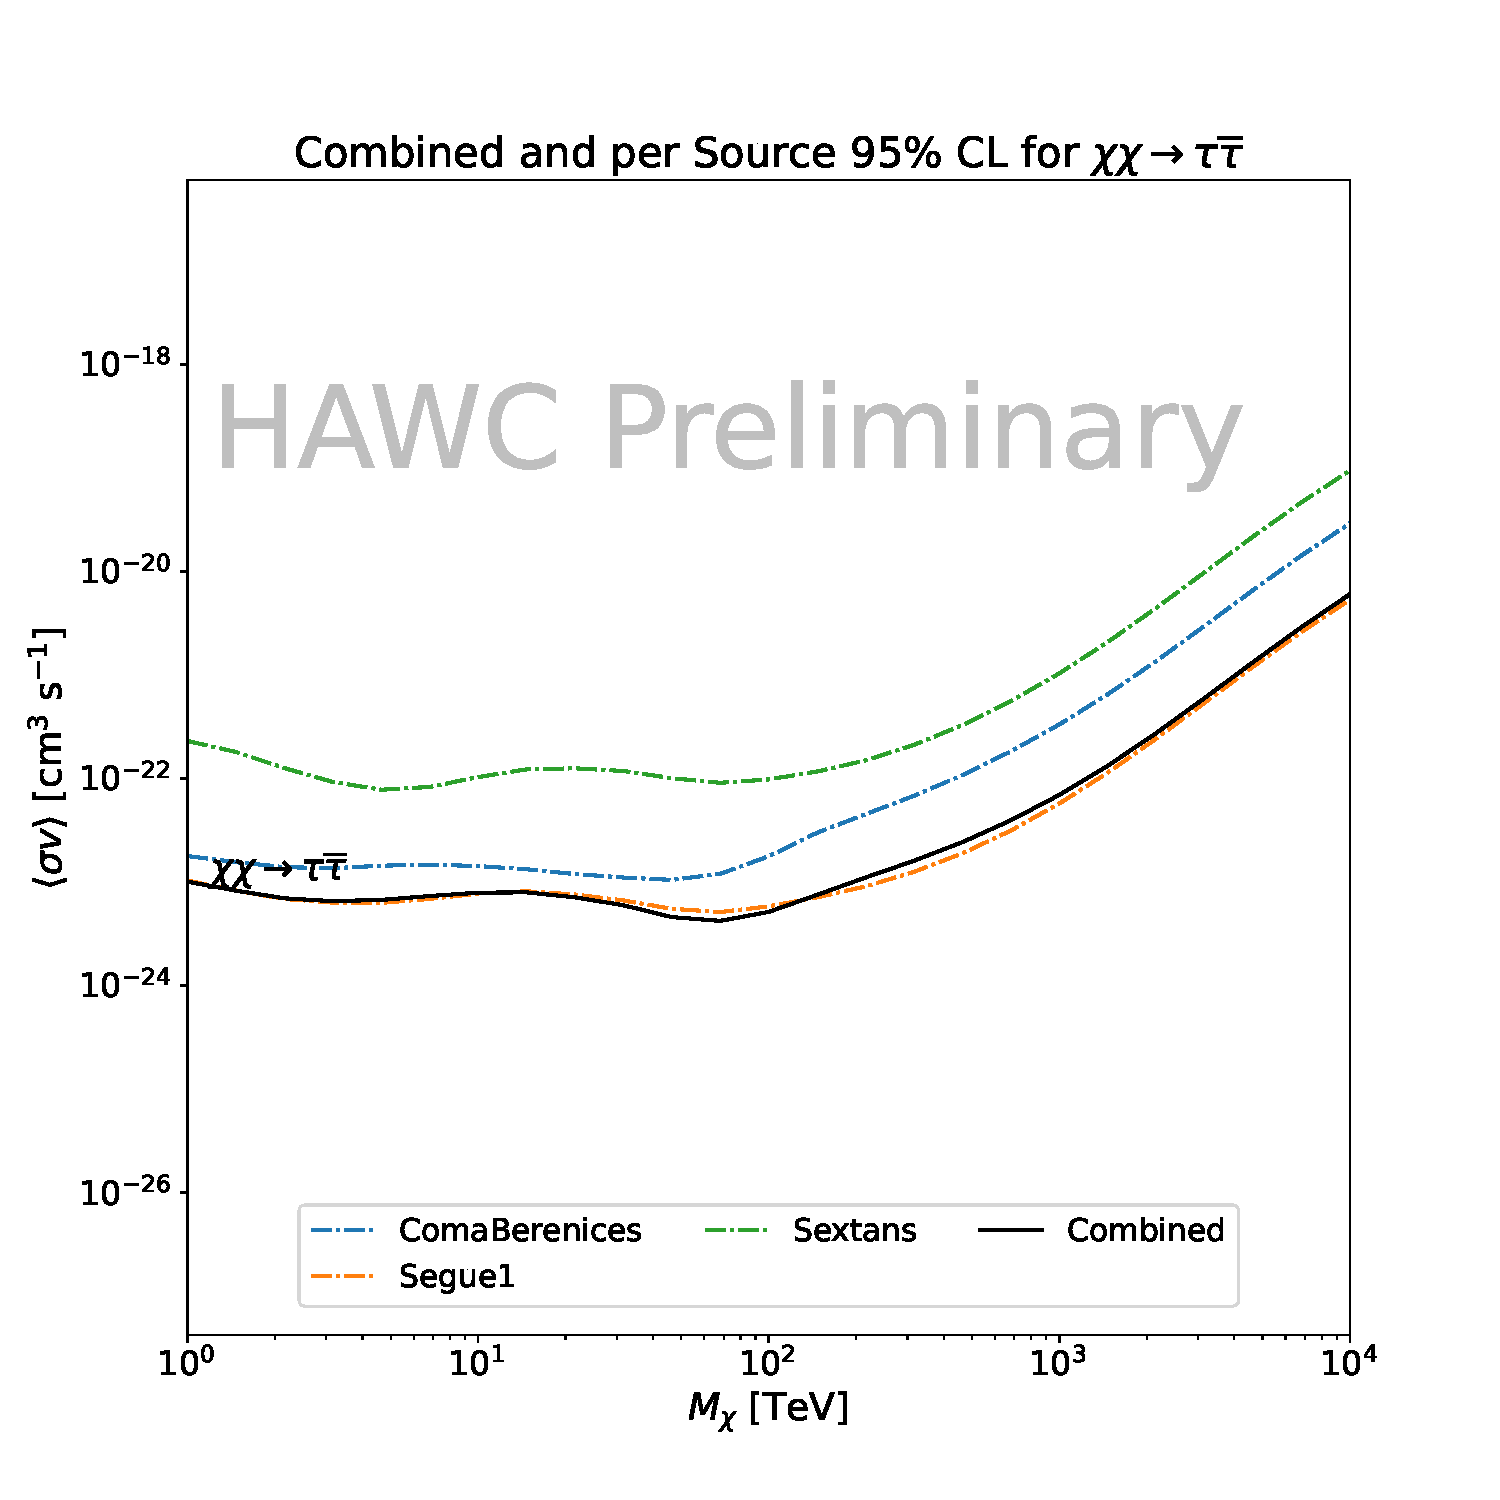
\includegraphics[scale=0.21]{figures/mtd_hawc_dm/results/Combined95_New_duck_tautau_.pdf}
    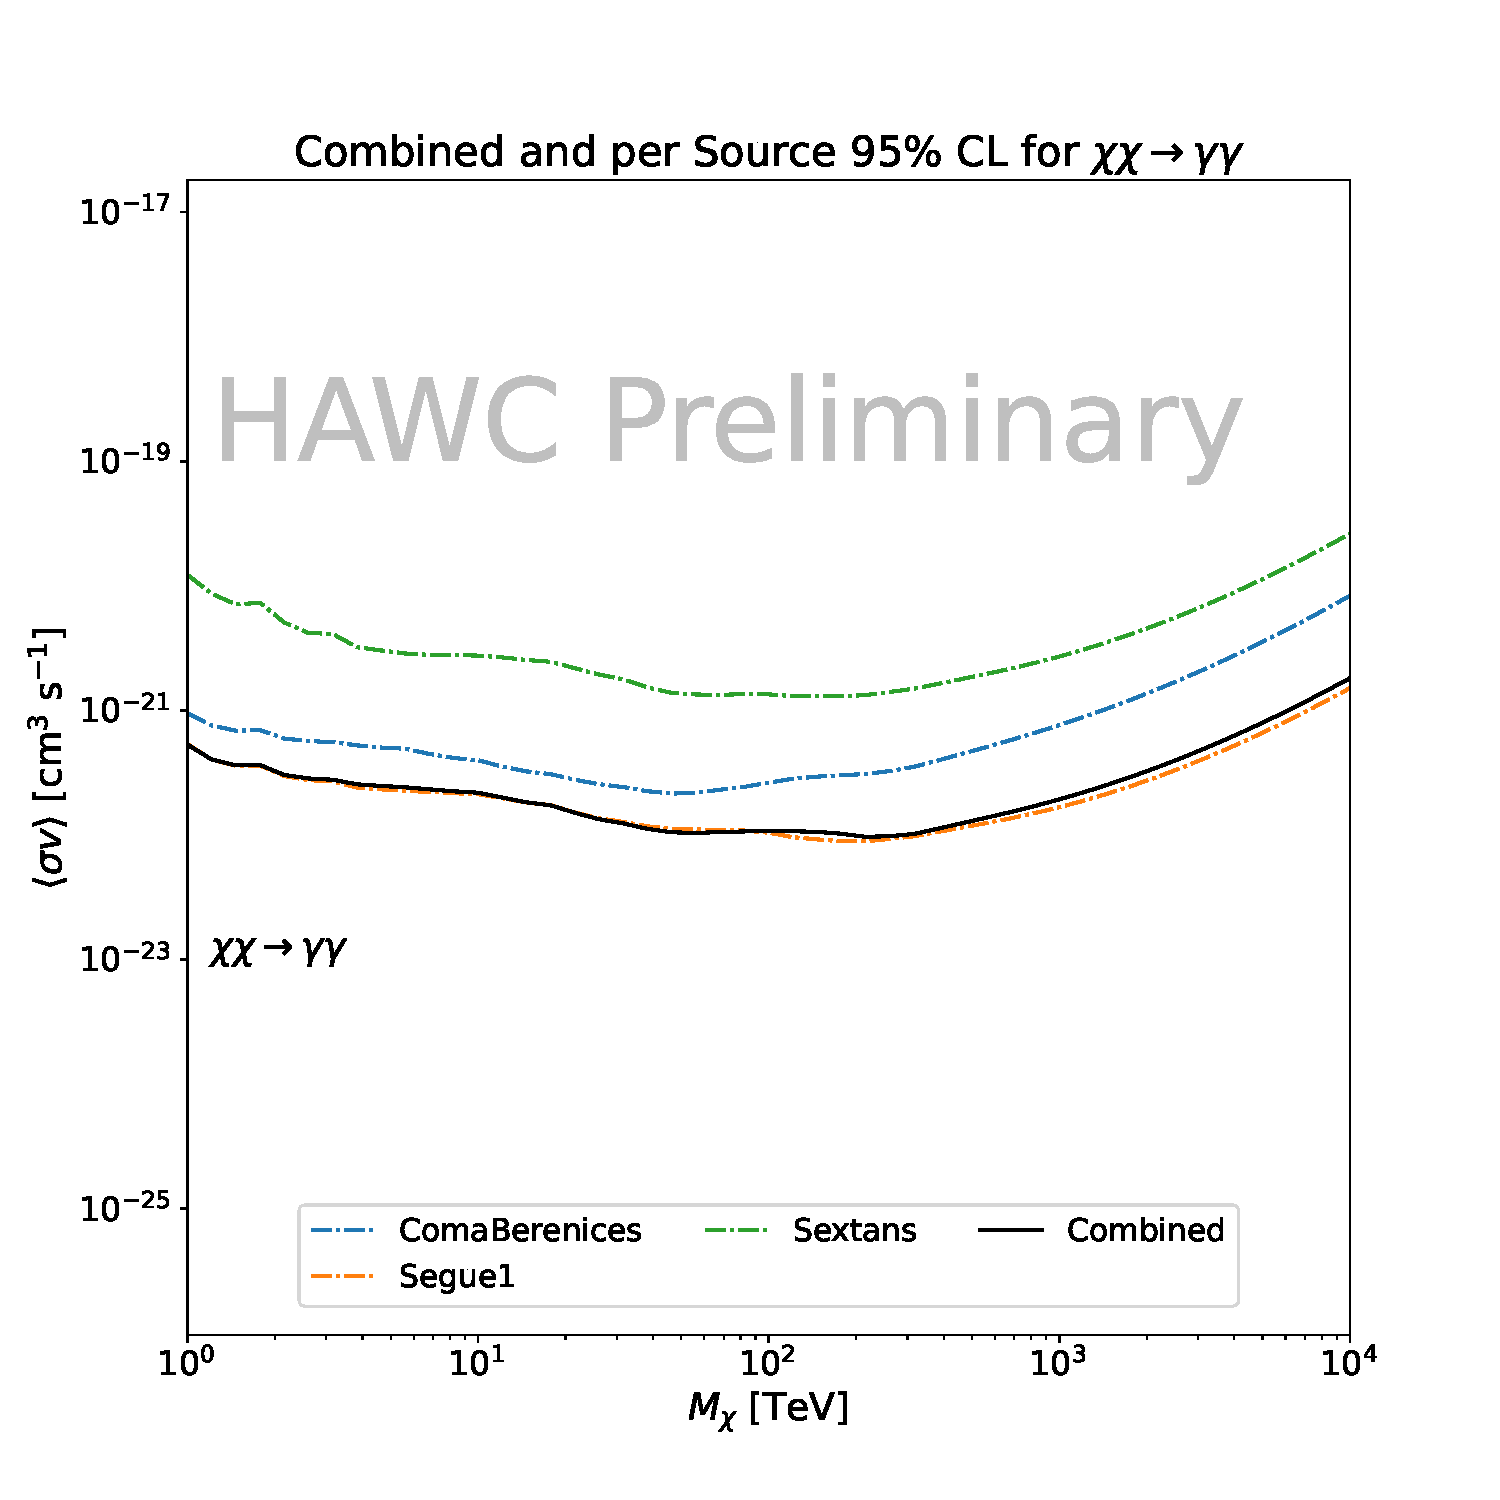
\includegraphics[scale=0.21]{figures/mtd_hawc_dm/results/Combined95_New_duck_gammagamma_.pdf}
    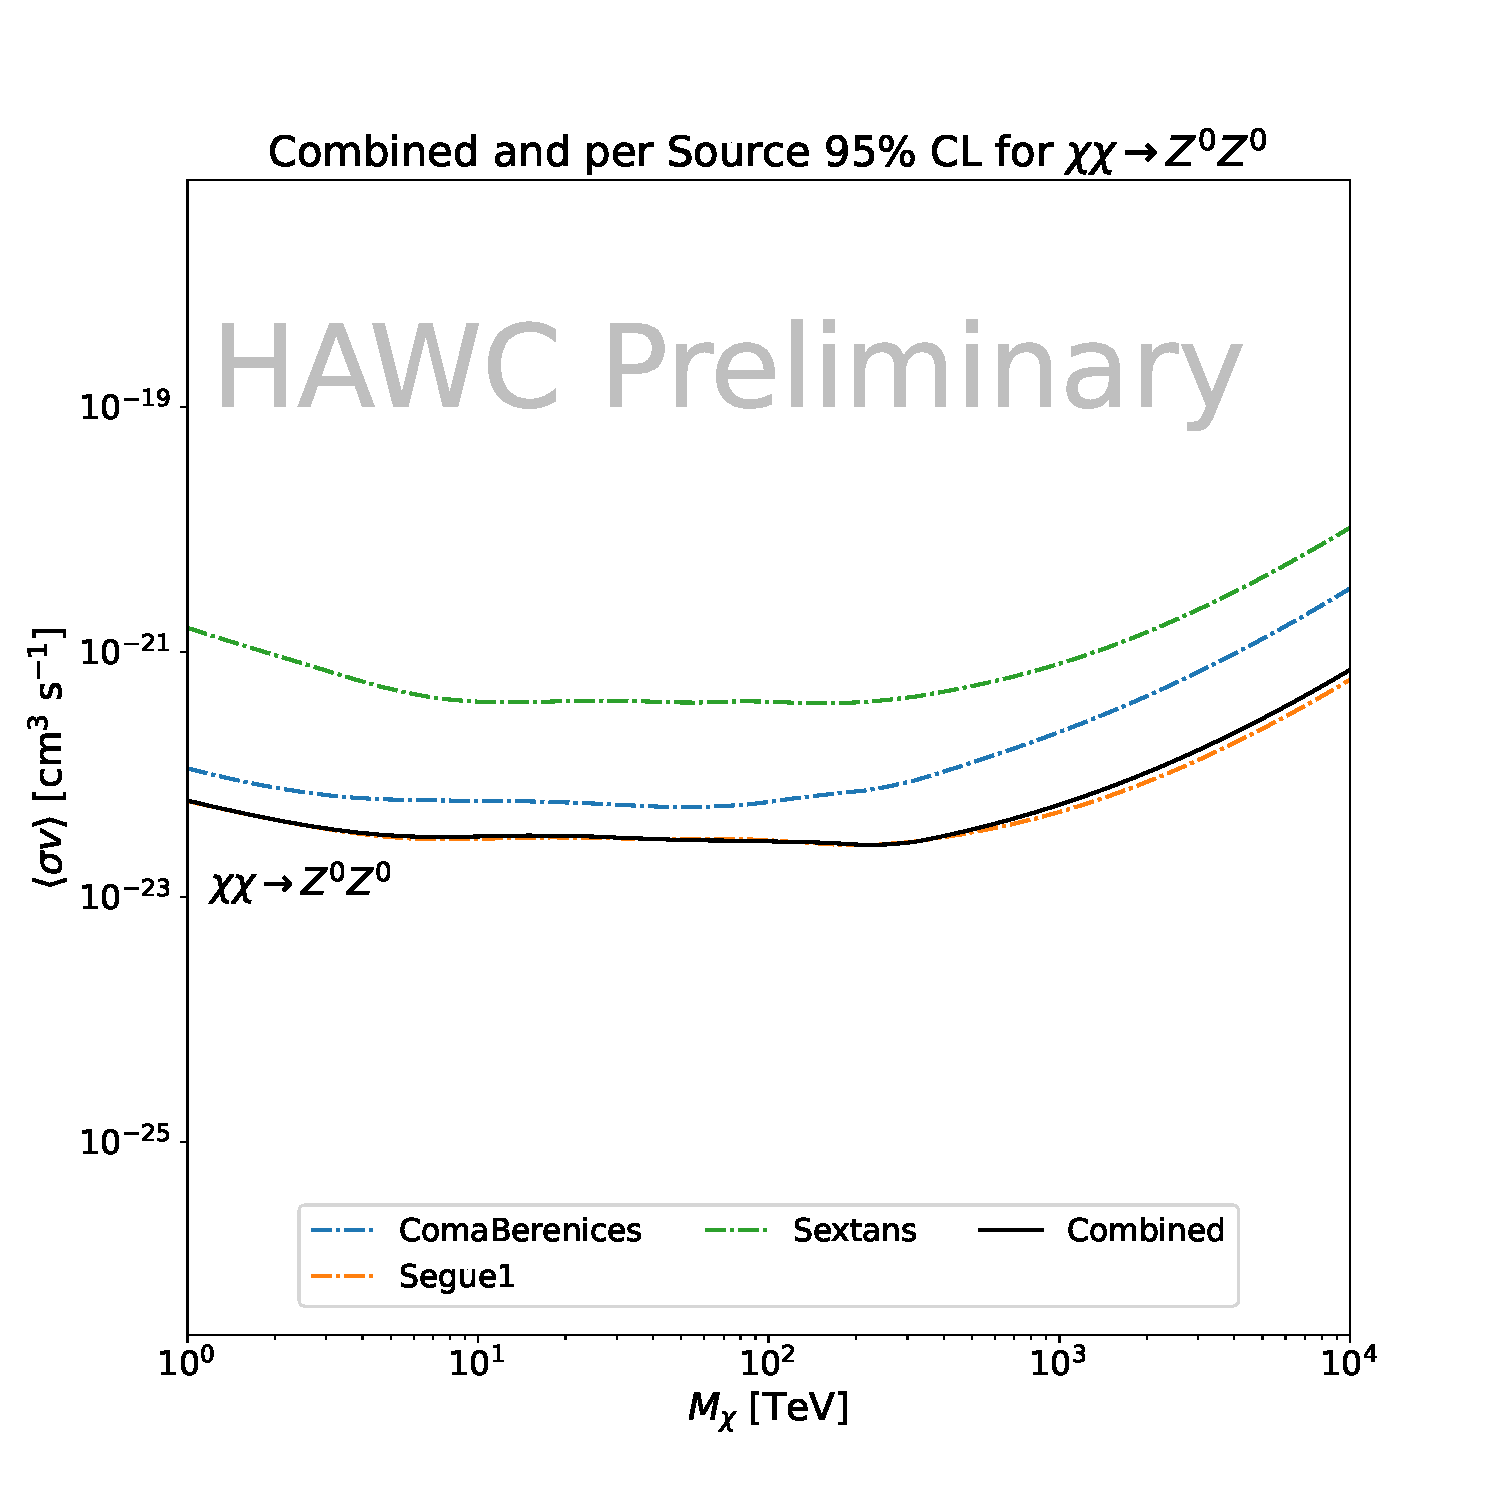
\includegraphics[scale=0.21]{figures/mtd_hawc_dm/results/Combined95_New_duck_zz_.pdf}
    }
    \caption{HAWC upper limits at 95\% confidence level on \sv~versus $m_\chi$ for $\chi\chi \rightarrow $ \parpar{\nu_e}, \parpar{\nu_\mu}, \parpar{\nu_\tau}, \parpar{e}, \parpar{\mu}, \parpar{\tau}, \pp{\gamma} and \pp{Z}. Limits use \LS \J-factors \cite{DM_Strigari20}. The solid line represents the observed combined limit. Dashed lines represent limits from individual dSphs.}
\label{fig:mtd_limits_2of2}
\end{figure}

\begin{figure}[h]
\centering{
    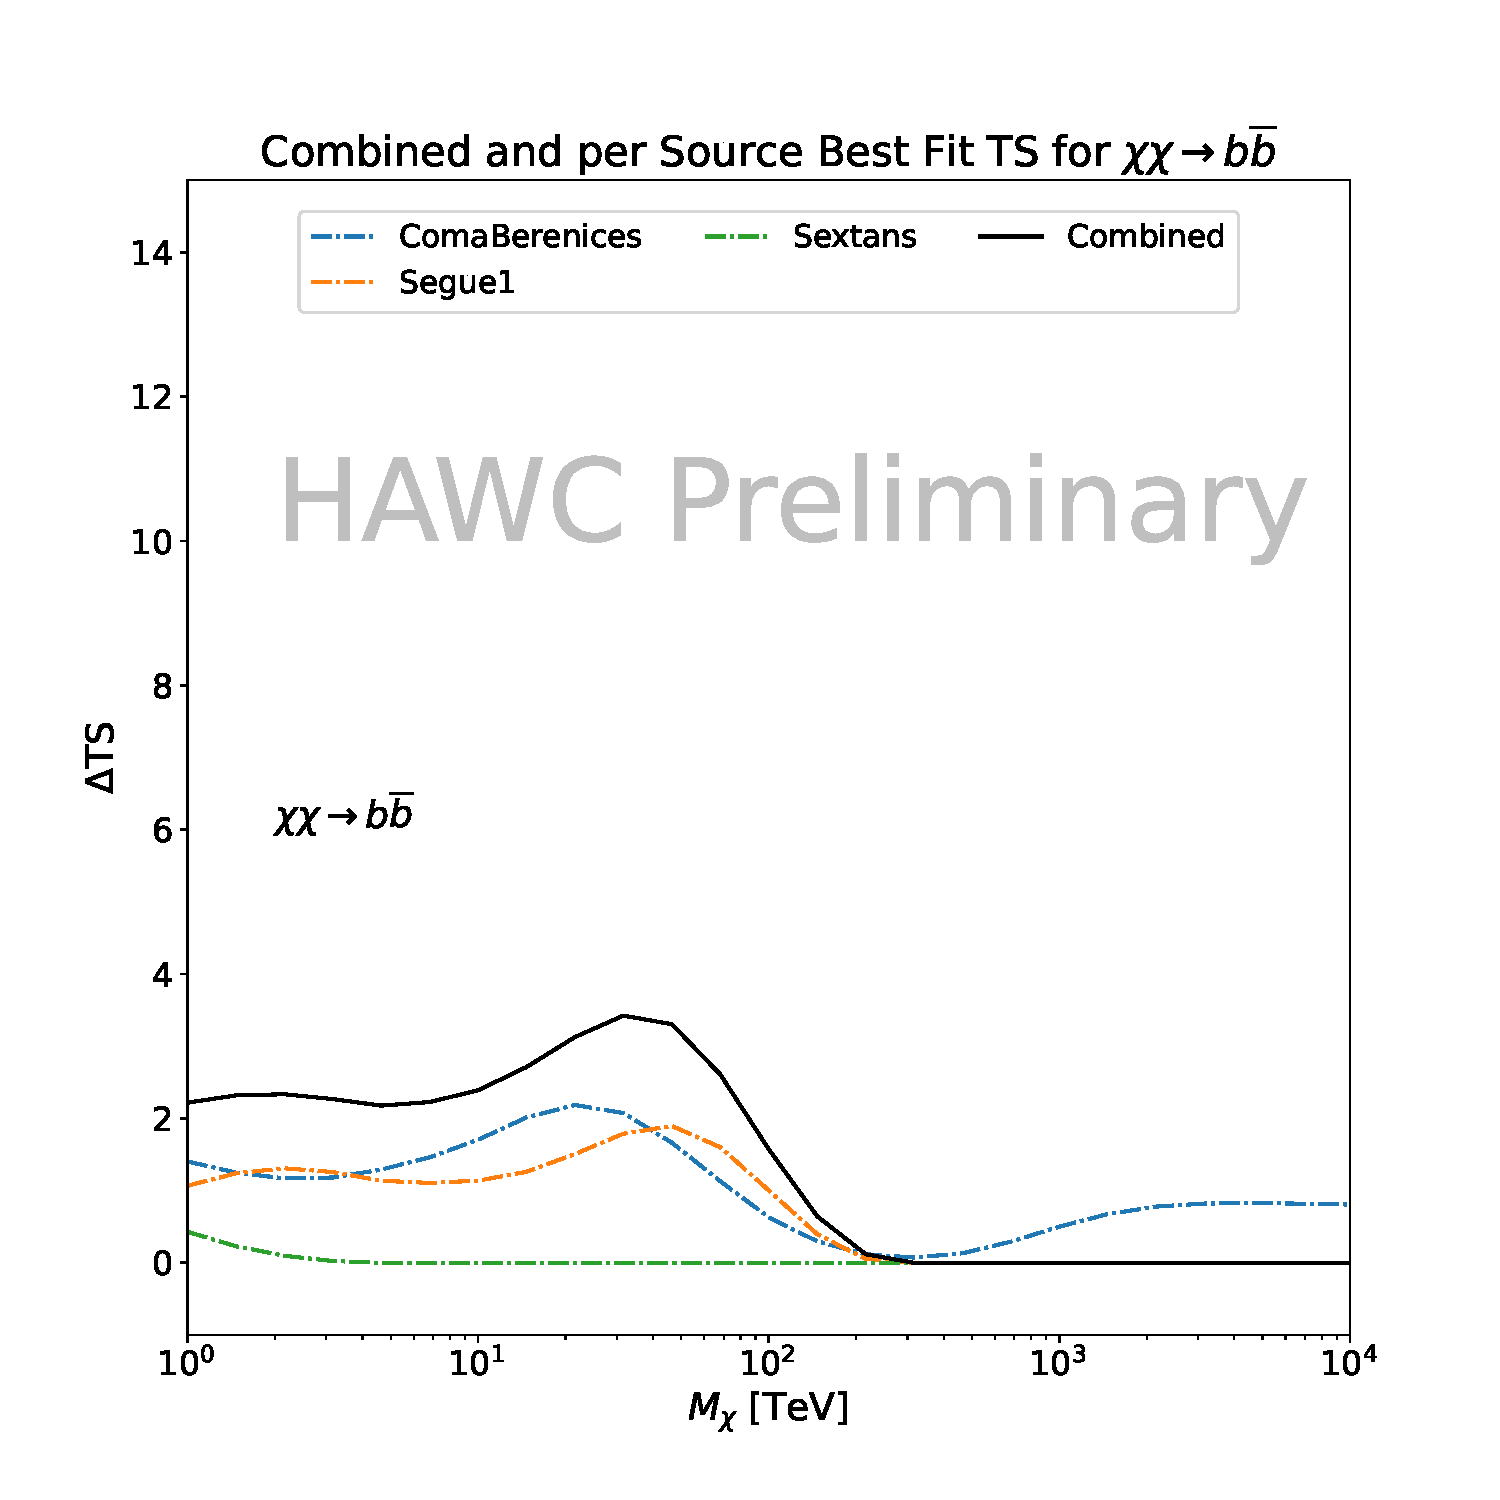
\includegraphics[scale=0.21]{figures/mtd_hawc_dm/results/CombinedTS_New_duck_bb_.pdf}
    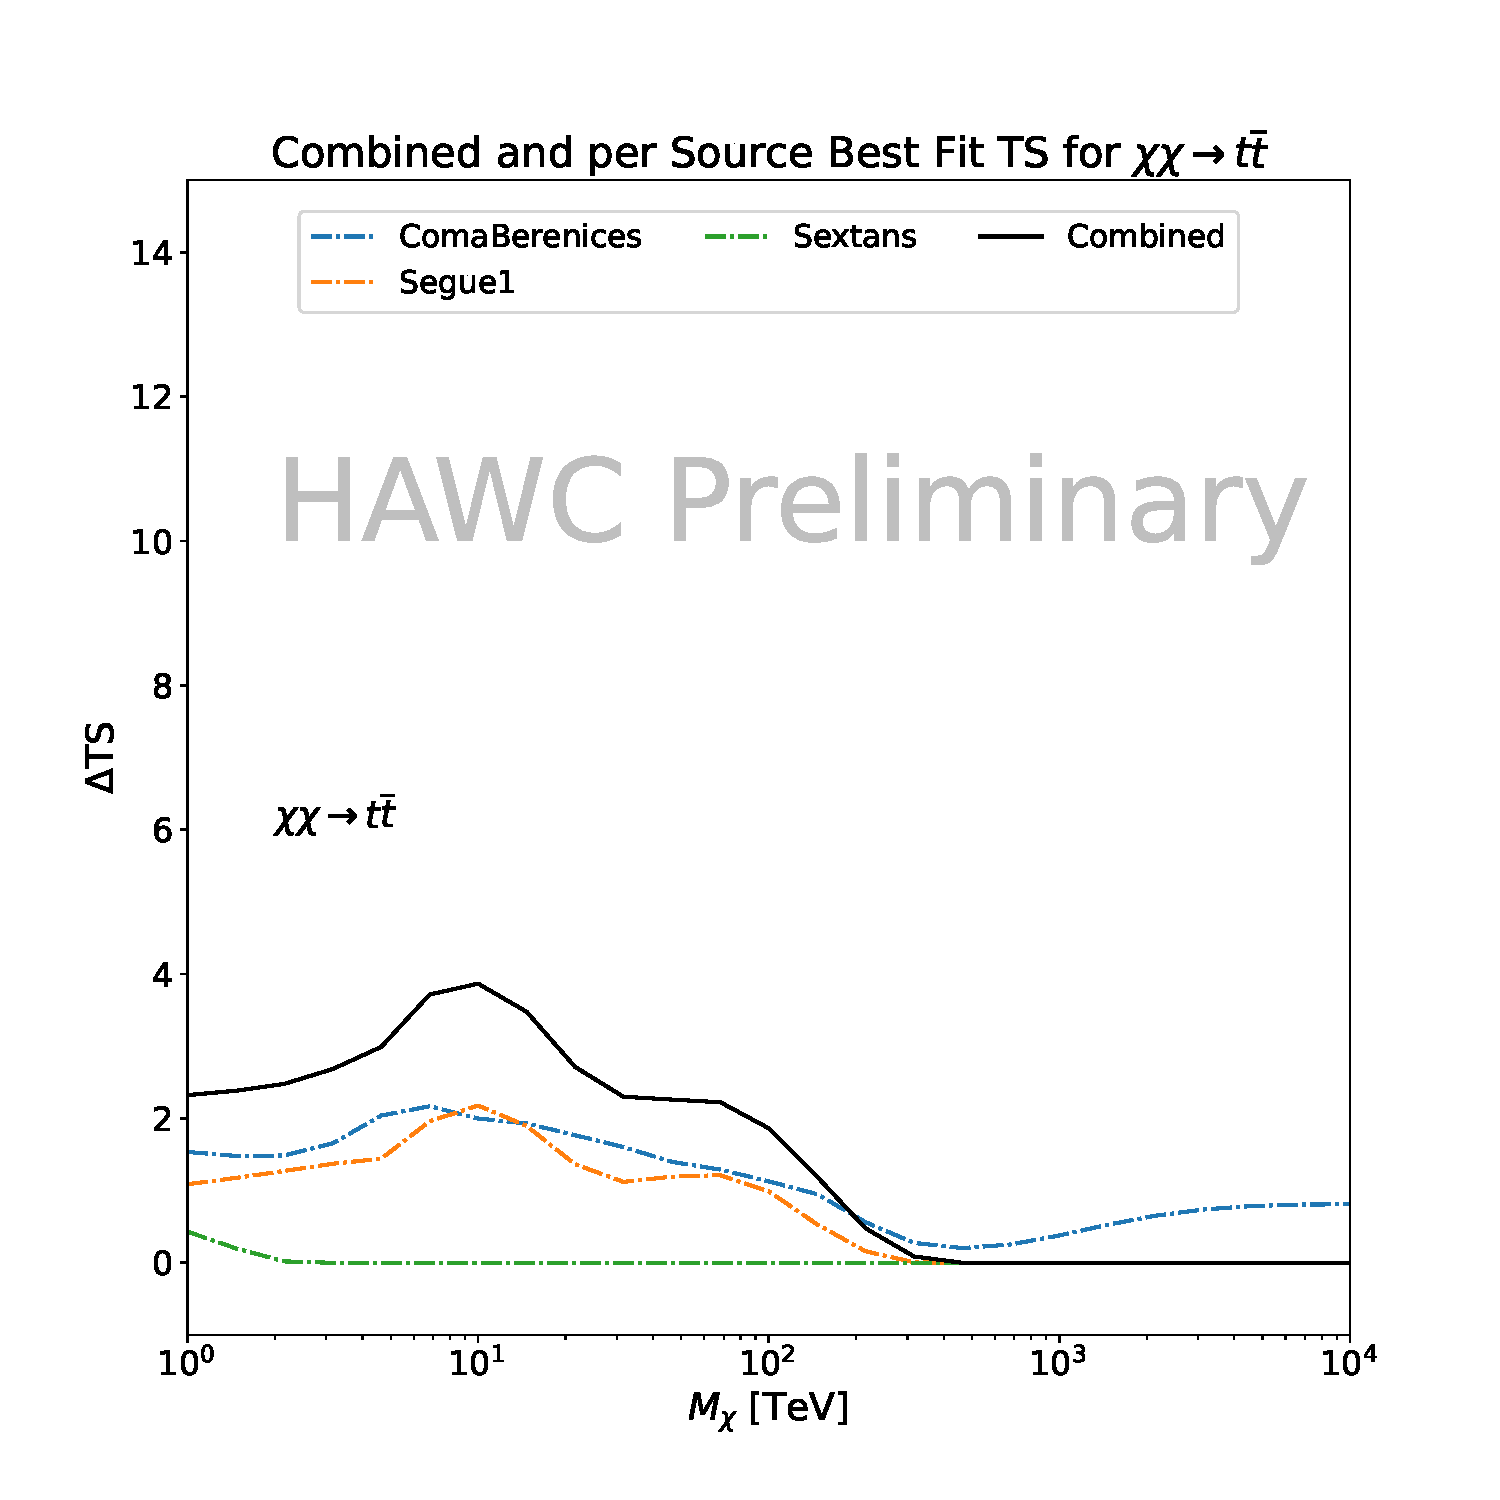
\includegraphics[scale=0.21]{figures/mtd_hawc_dm/results/CombinedTS_New_duck_tt_.pdf}
    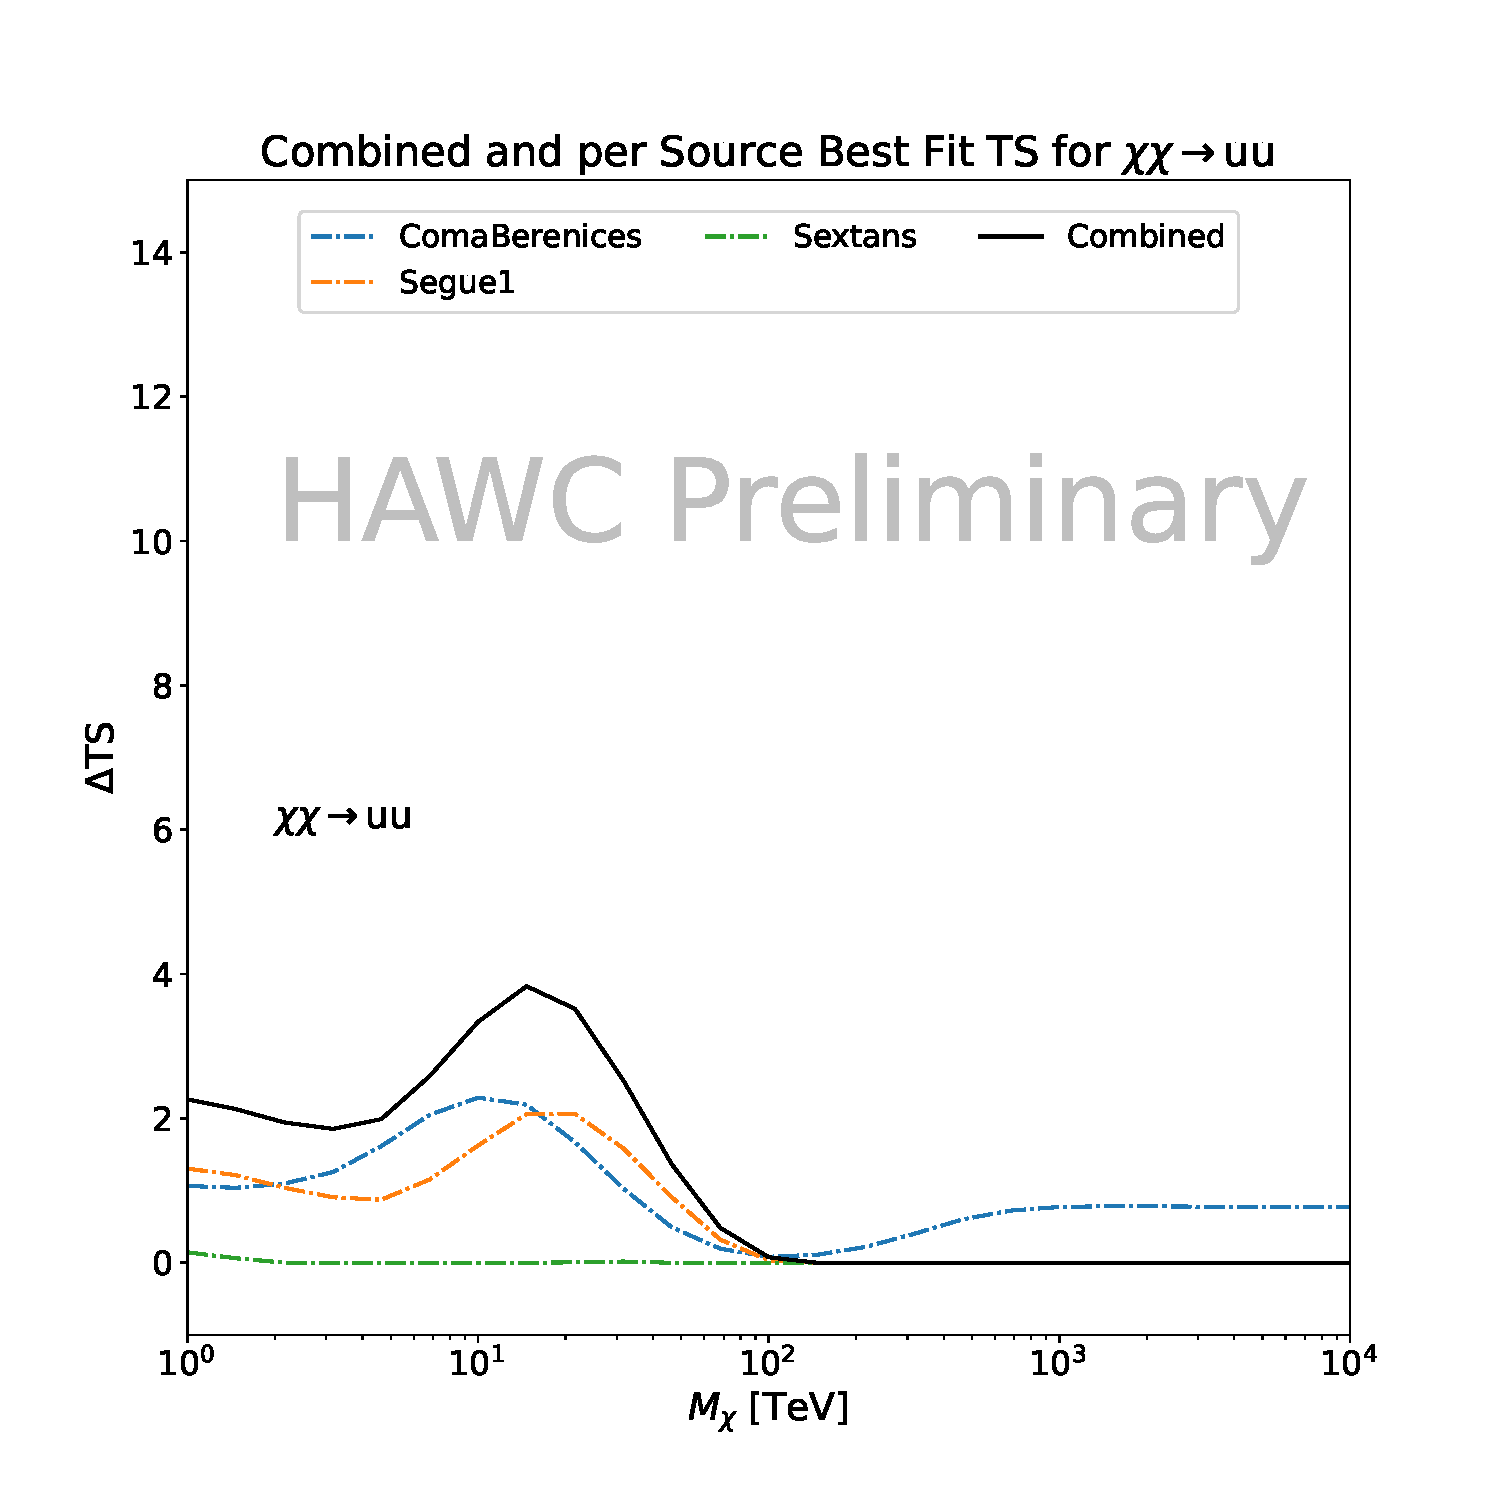
\includegraphics[scale=0.21]{figures/mtd_hawc_dm/results/CombinedTS_New_duck_uu_.pdf}
    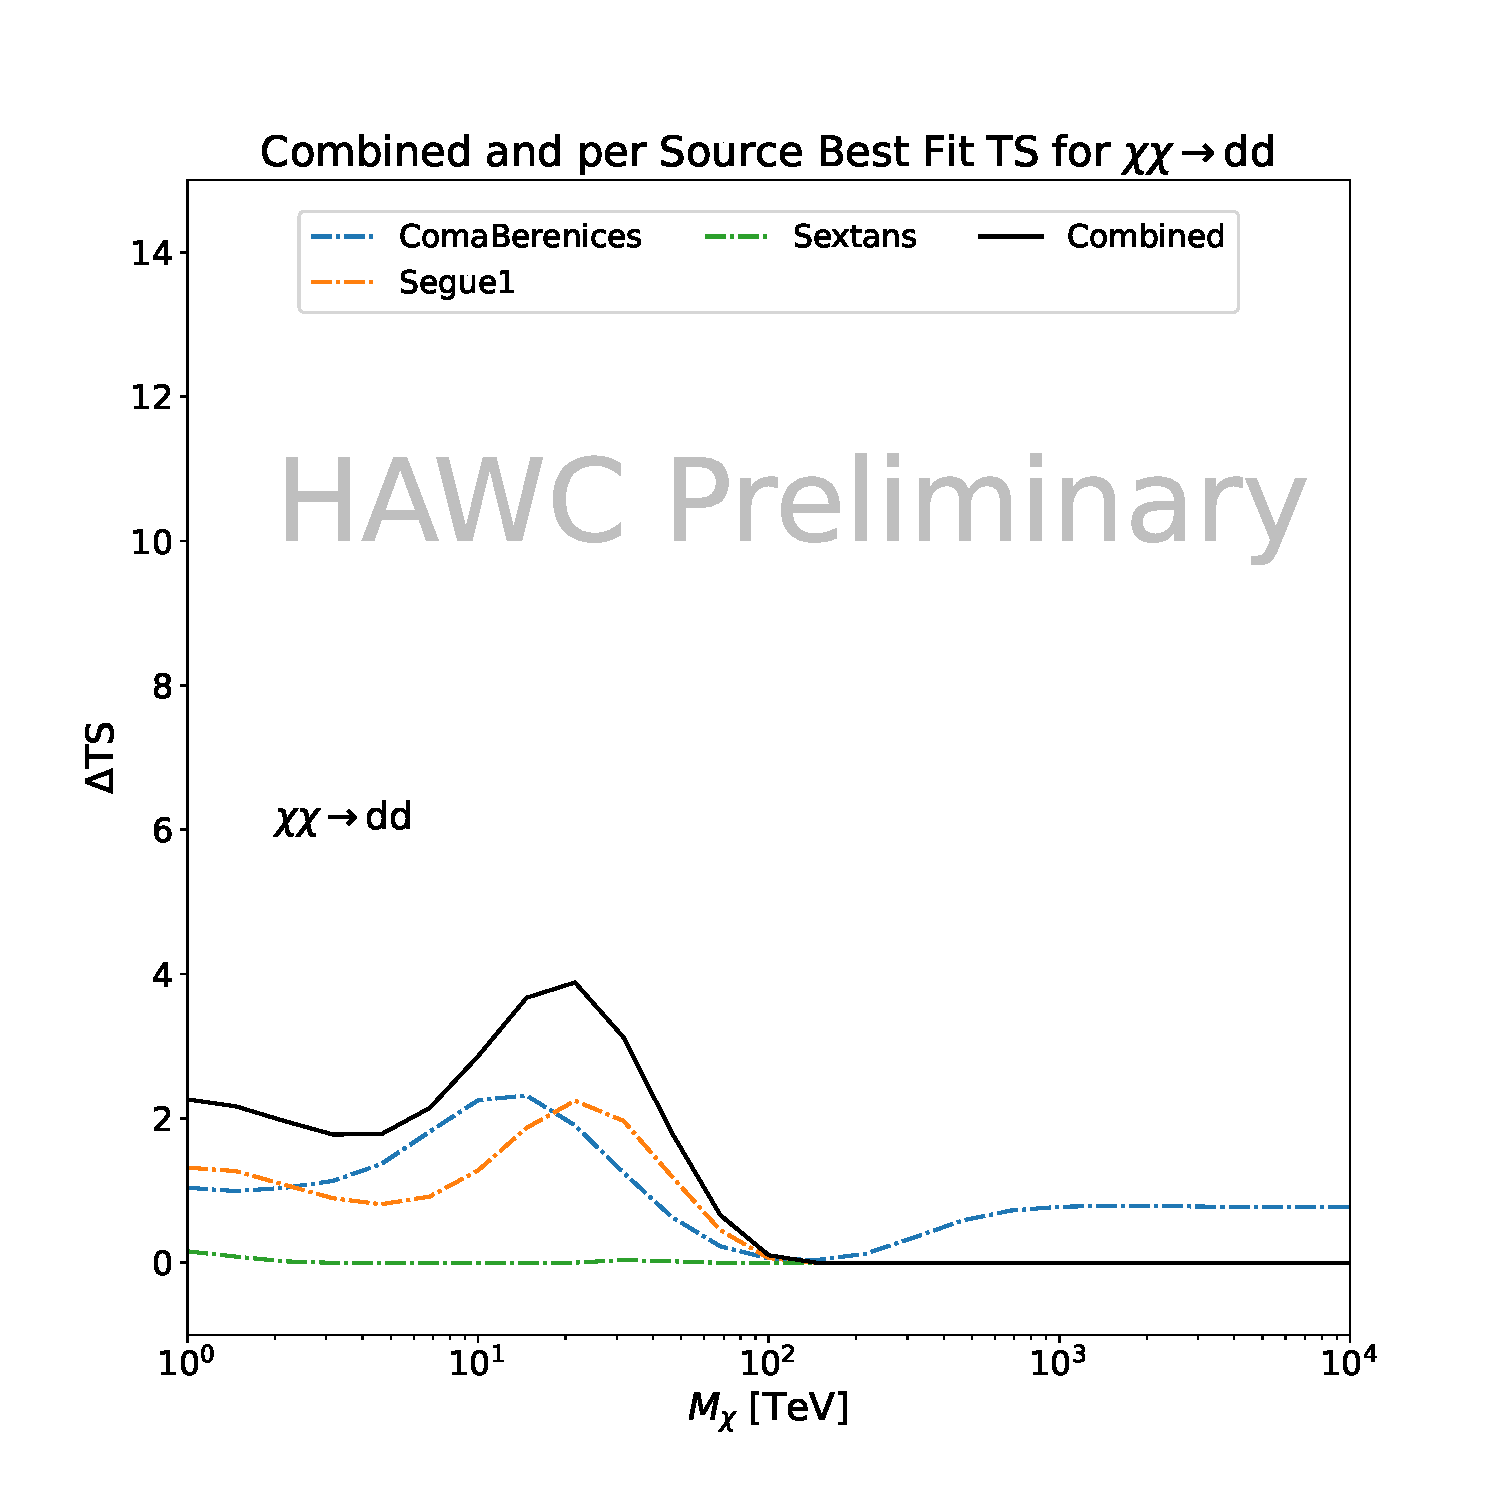
\includegraphics[scale=0.21]{figures/mtd_hawc_dm/results/CombinedTS_New_duck_dd_.pdf}
    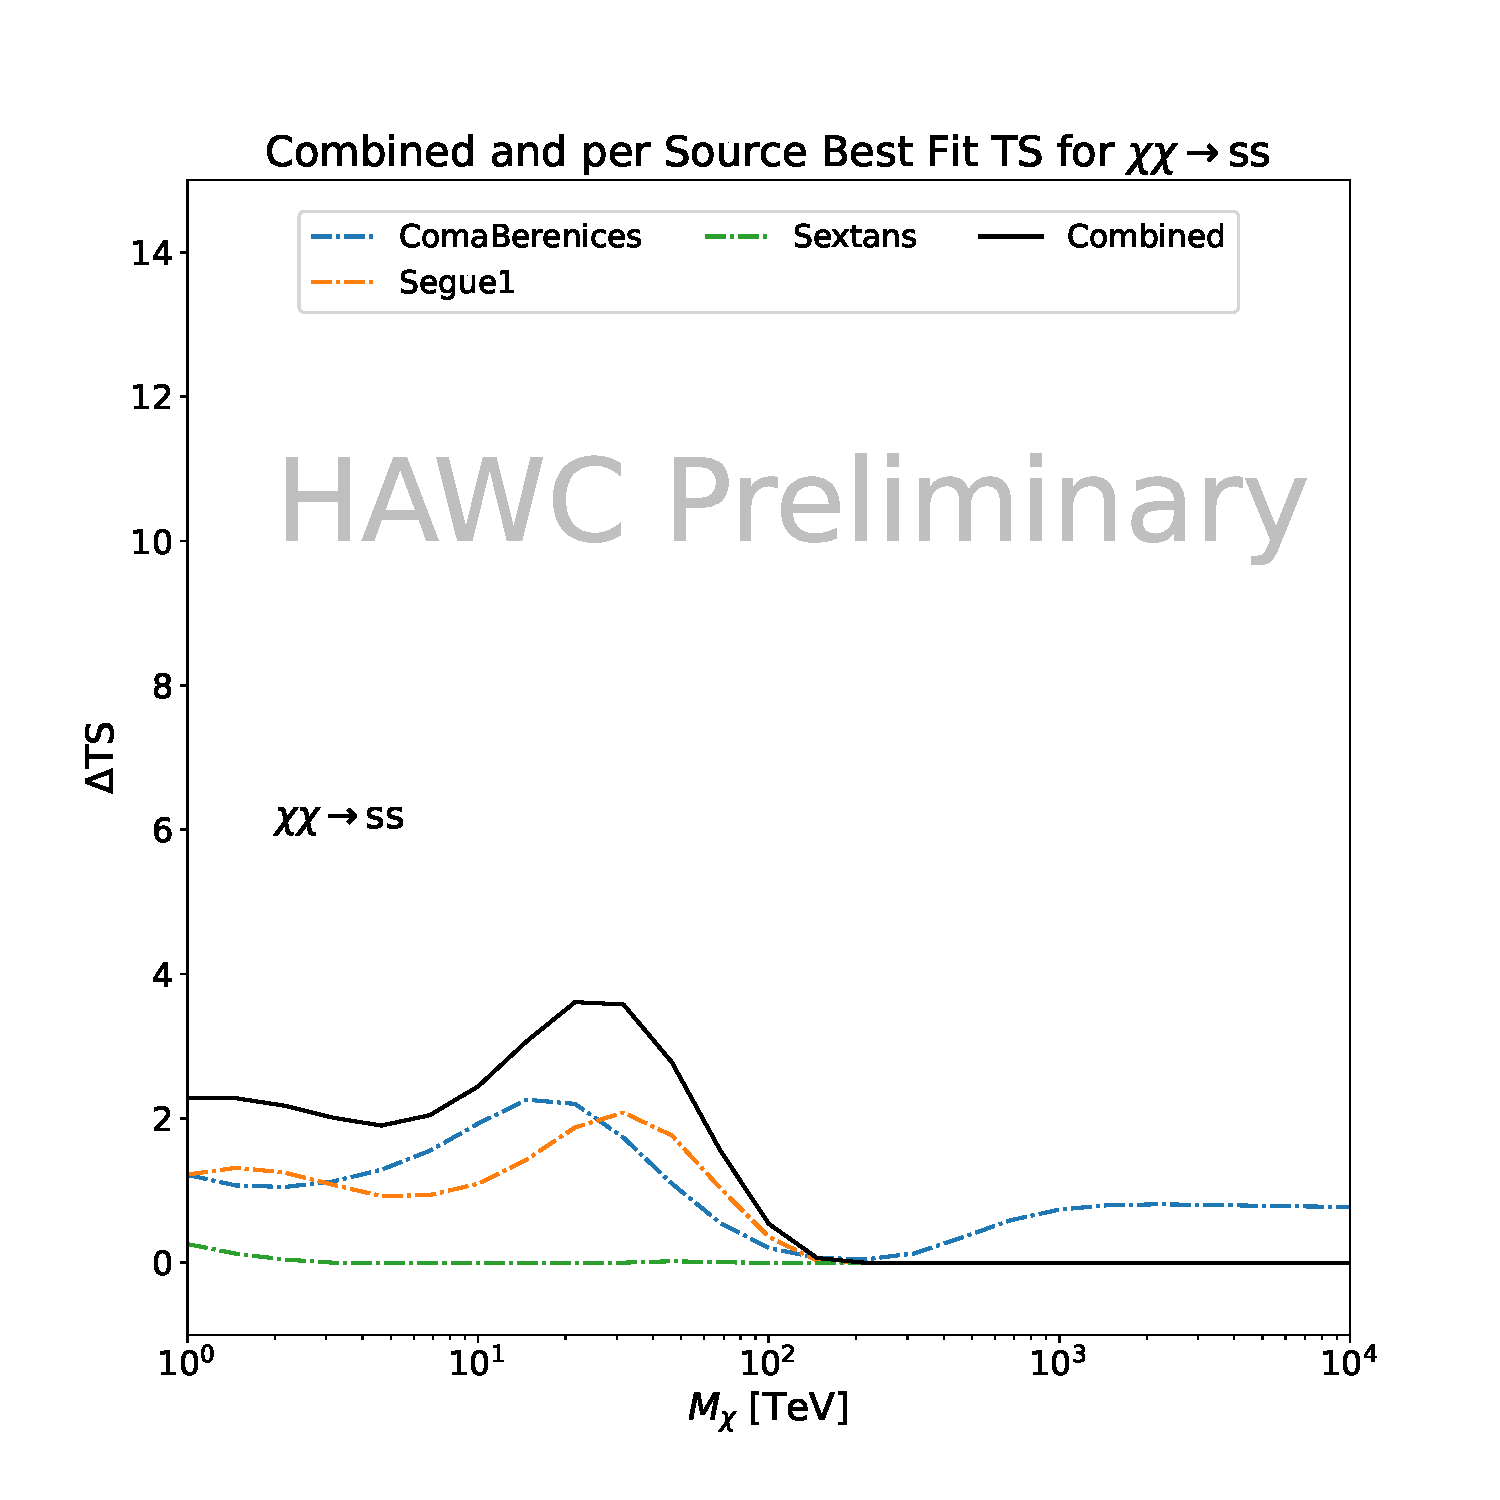
\includegraphics[scale=0.21]{figures/mtd_hawc_dm/results/CombinedTS_New_duck_ss_.pdf}
    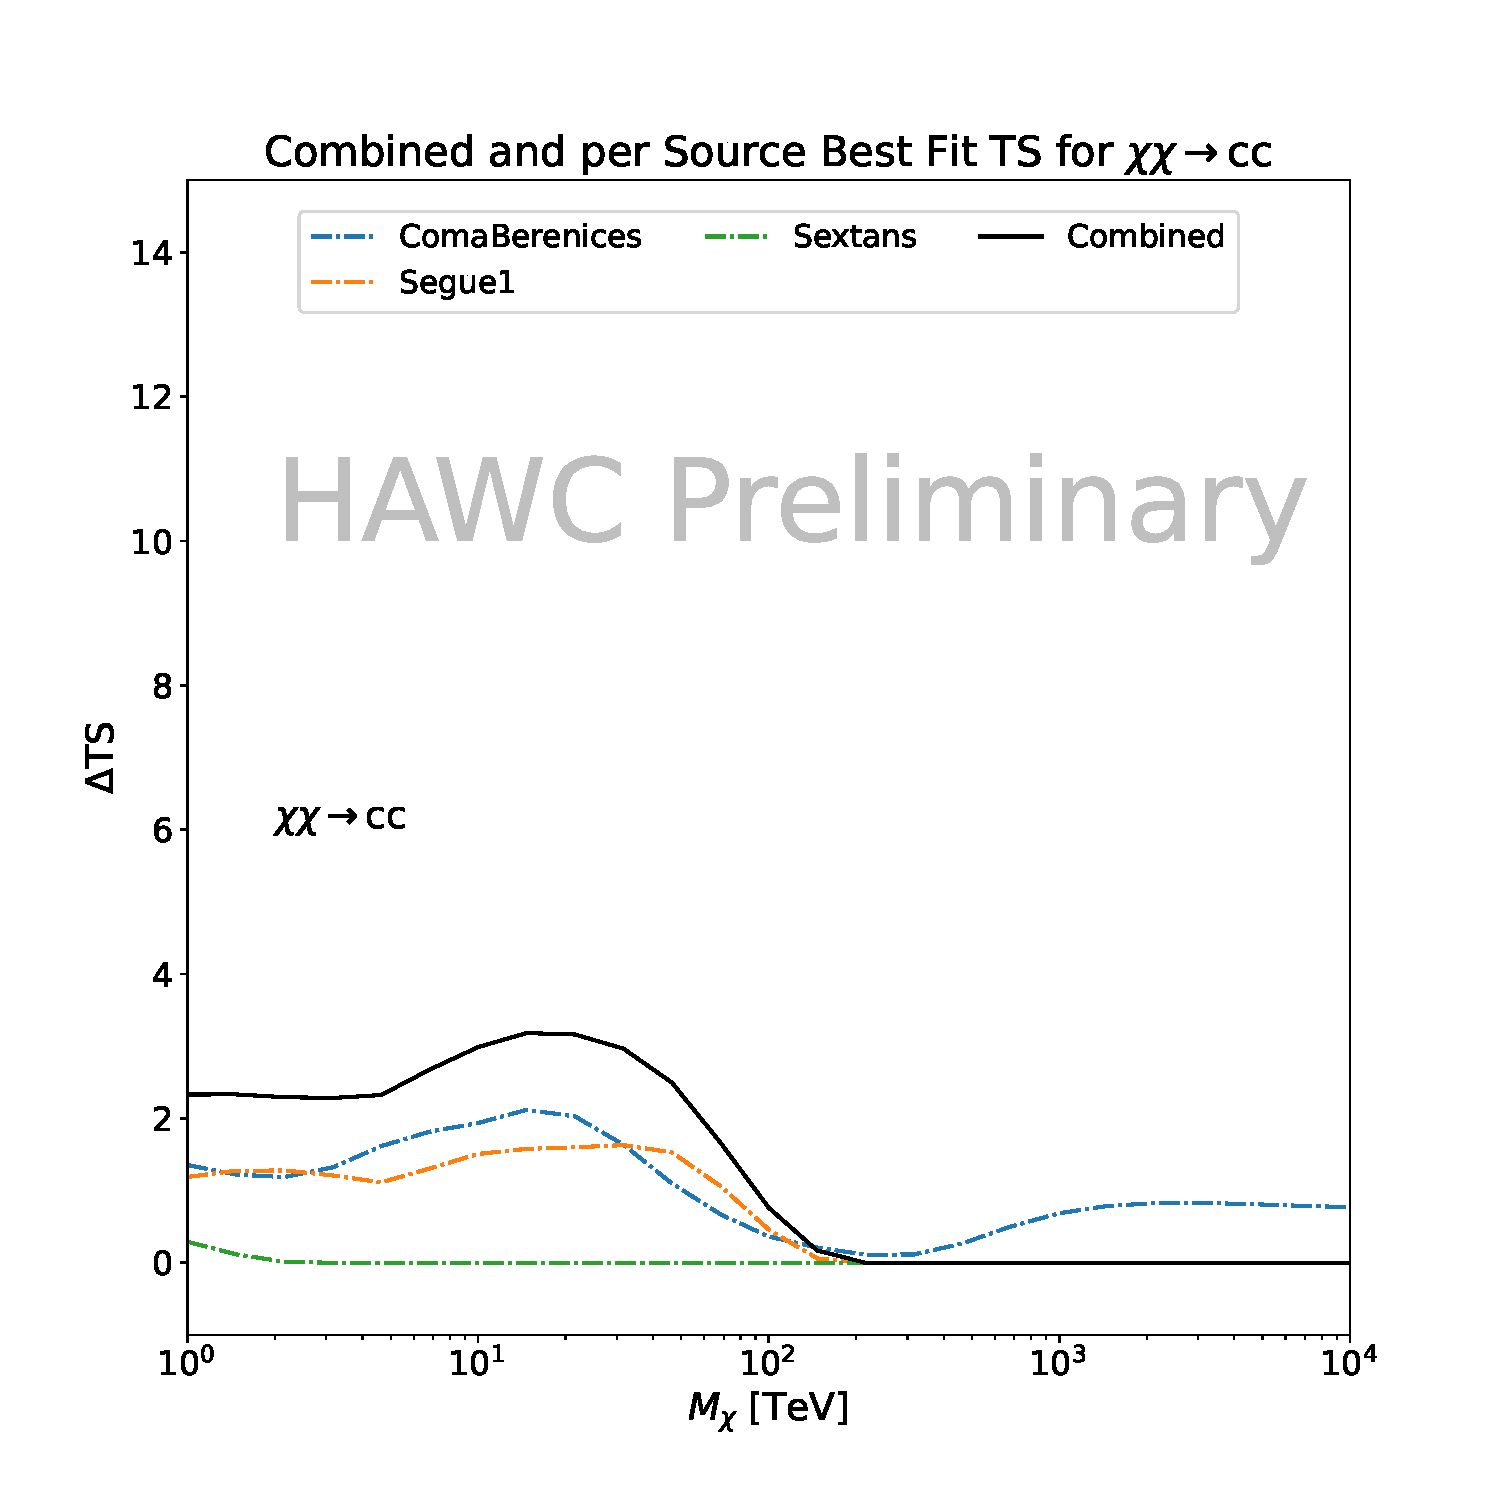
\includegraphics[scale=0.21]{figures/mtd_hawc_dm/results/CombinedTS_New_duck_cc_.pdf}
    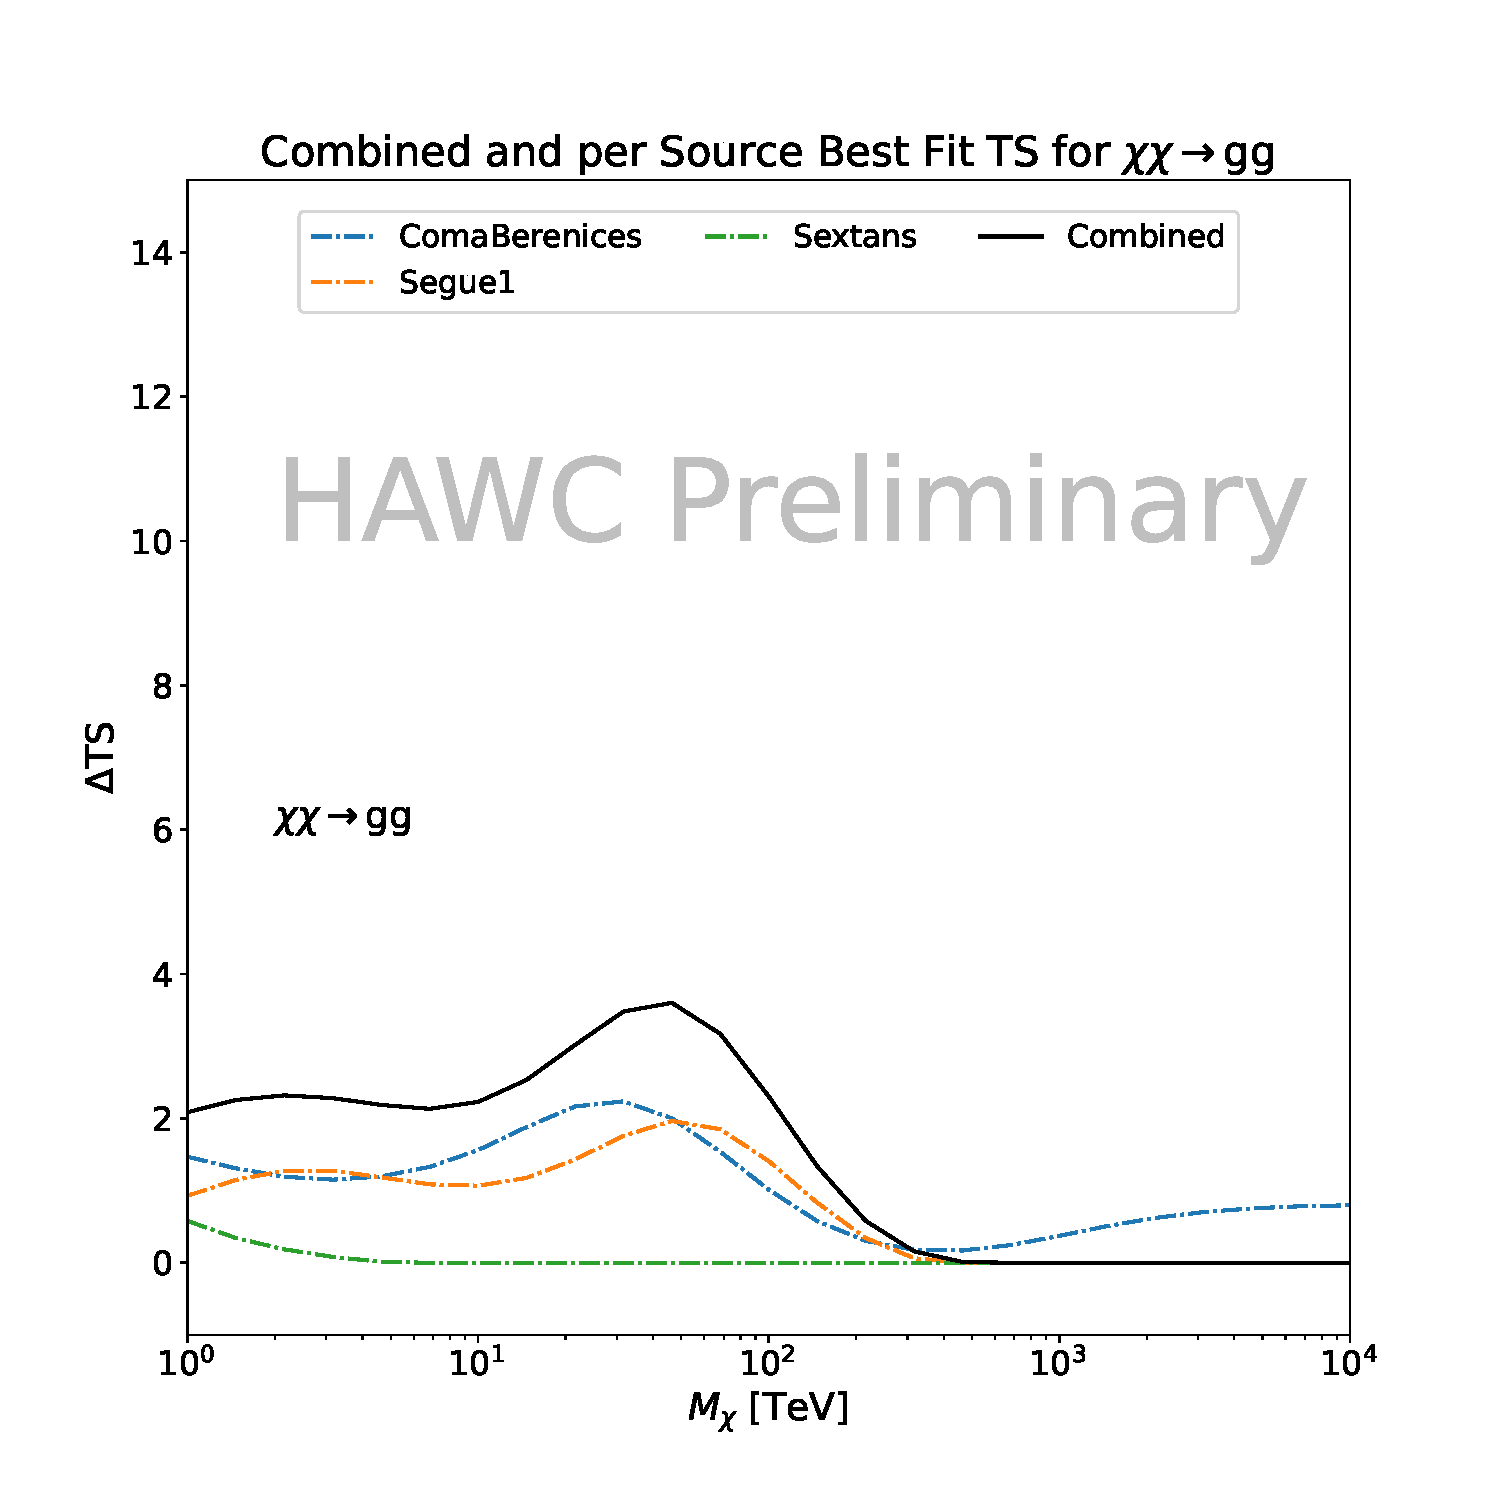
\includegraphics[scale=0.21]{figures/mtd_hawc_dm/results/CombinedTS_New_duck_gg_.pdf}
    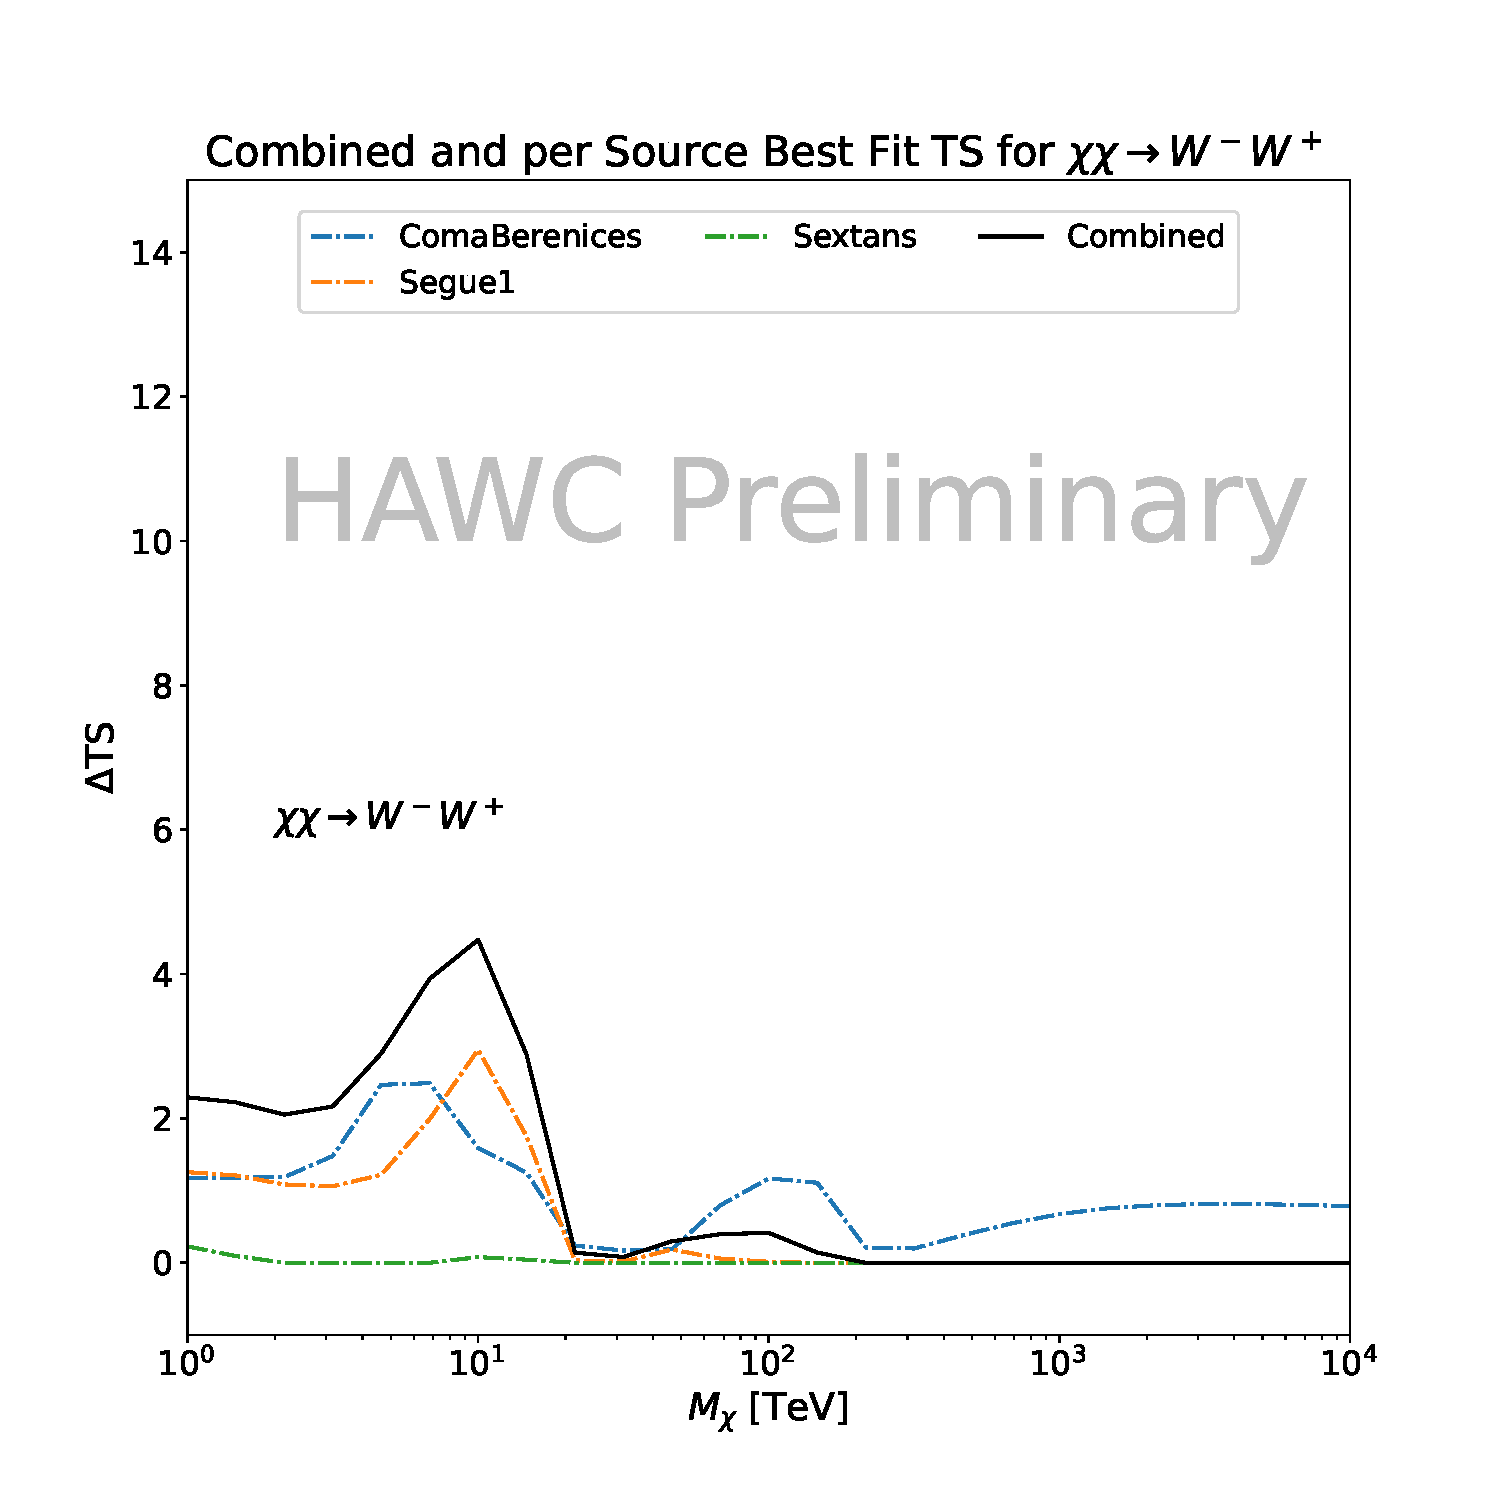
\includegraphics[scale=0.21]{figures/mtd_hawc_dm/results/CombinedTS_New_duck_ww_.pdf}
    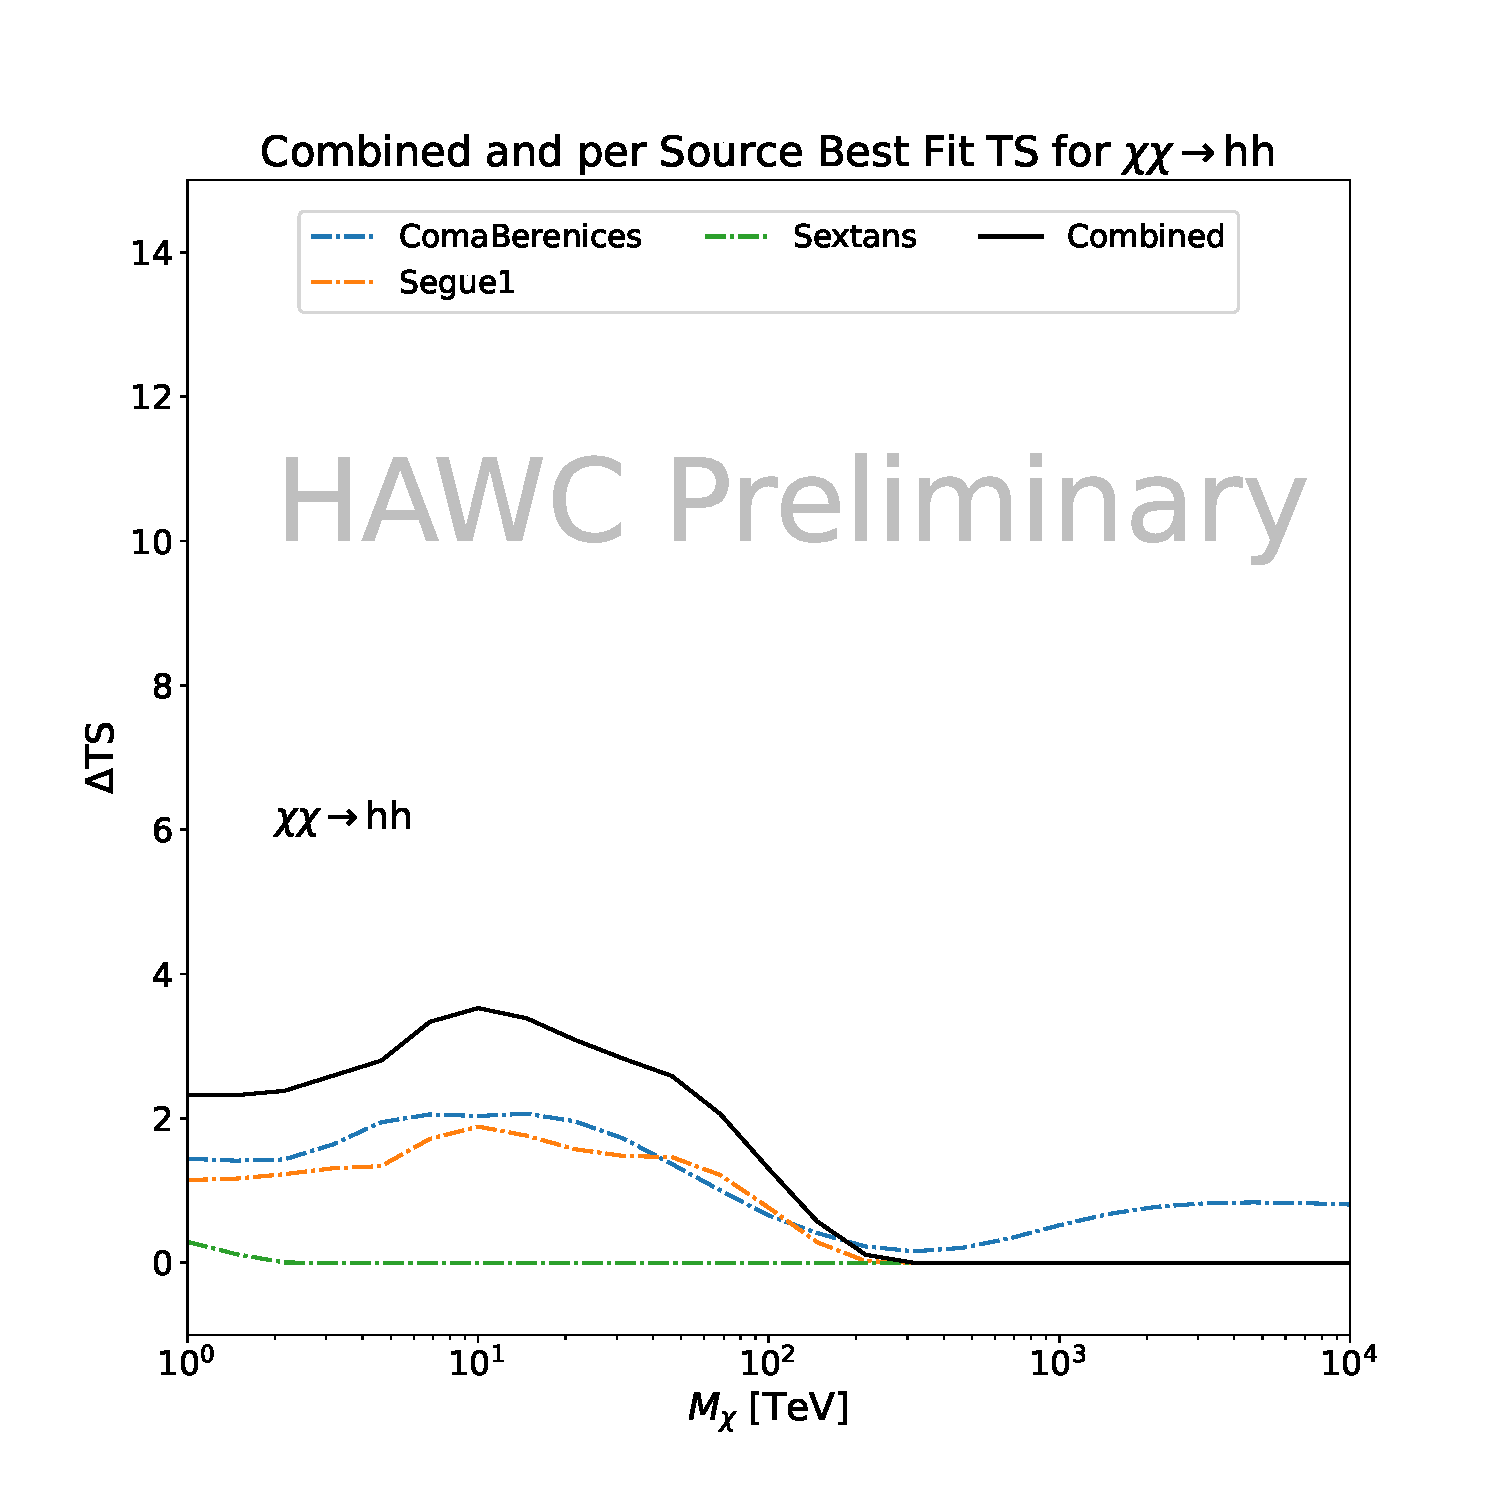
\includegraphics[scale=0.21]{figures/mtd_hawc_dm/results/CombinedTS_New_duck_hh_.pdf}
    }
    \caption{HAWC TS values for best fit \sv~versus $m_\chi$ for SM annihilation channels: $\chi\chi \rightarrow $ \parpar{b}, \parpar{t}, \parpar{u}, \parpar{d}, \parpar{s}, \parpar{c}, \pp{g}, $W^+ W^-$, and \pp{h}. Limits use \LS \J-factors. The solid black line shows the combined best fit TS values. The colored, dashed lines are the TS values from each dSph.}
\label{fig:mtd_TS_1of2}
\end{figure}

\begin{figure}[h]
\centering{
    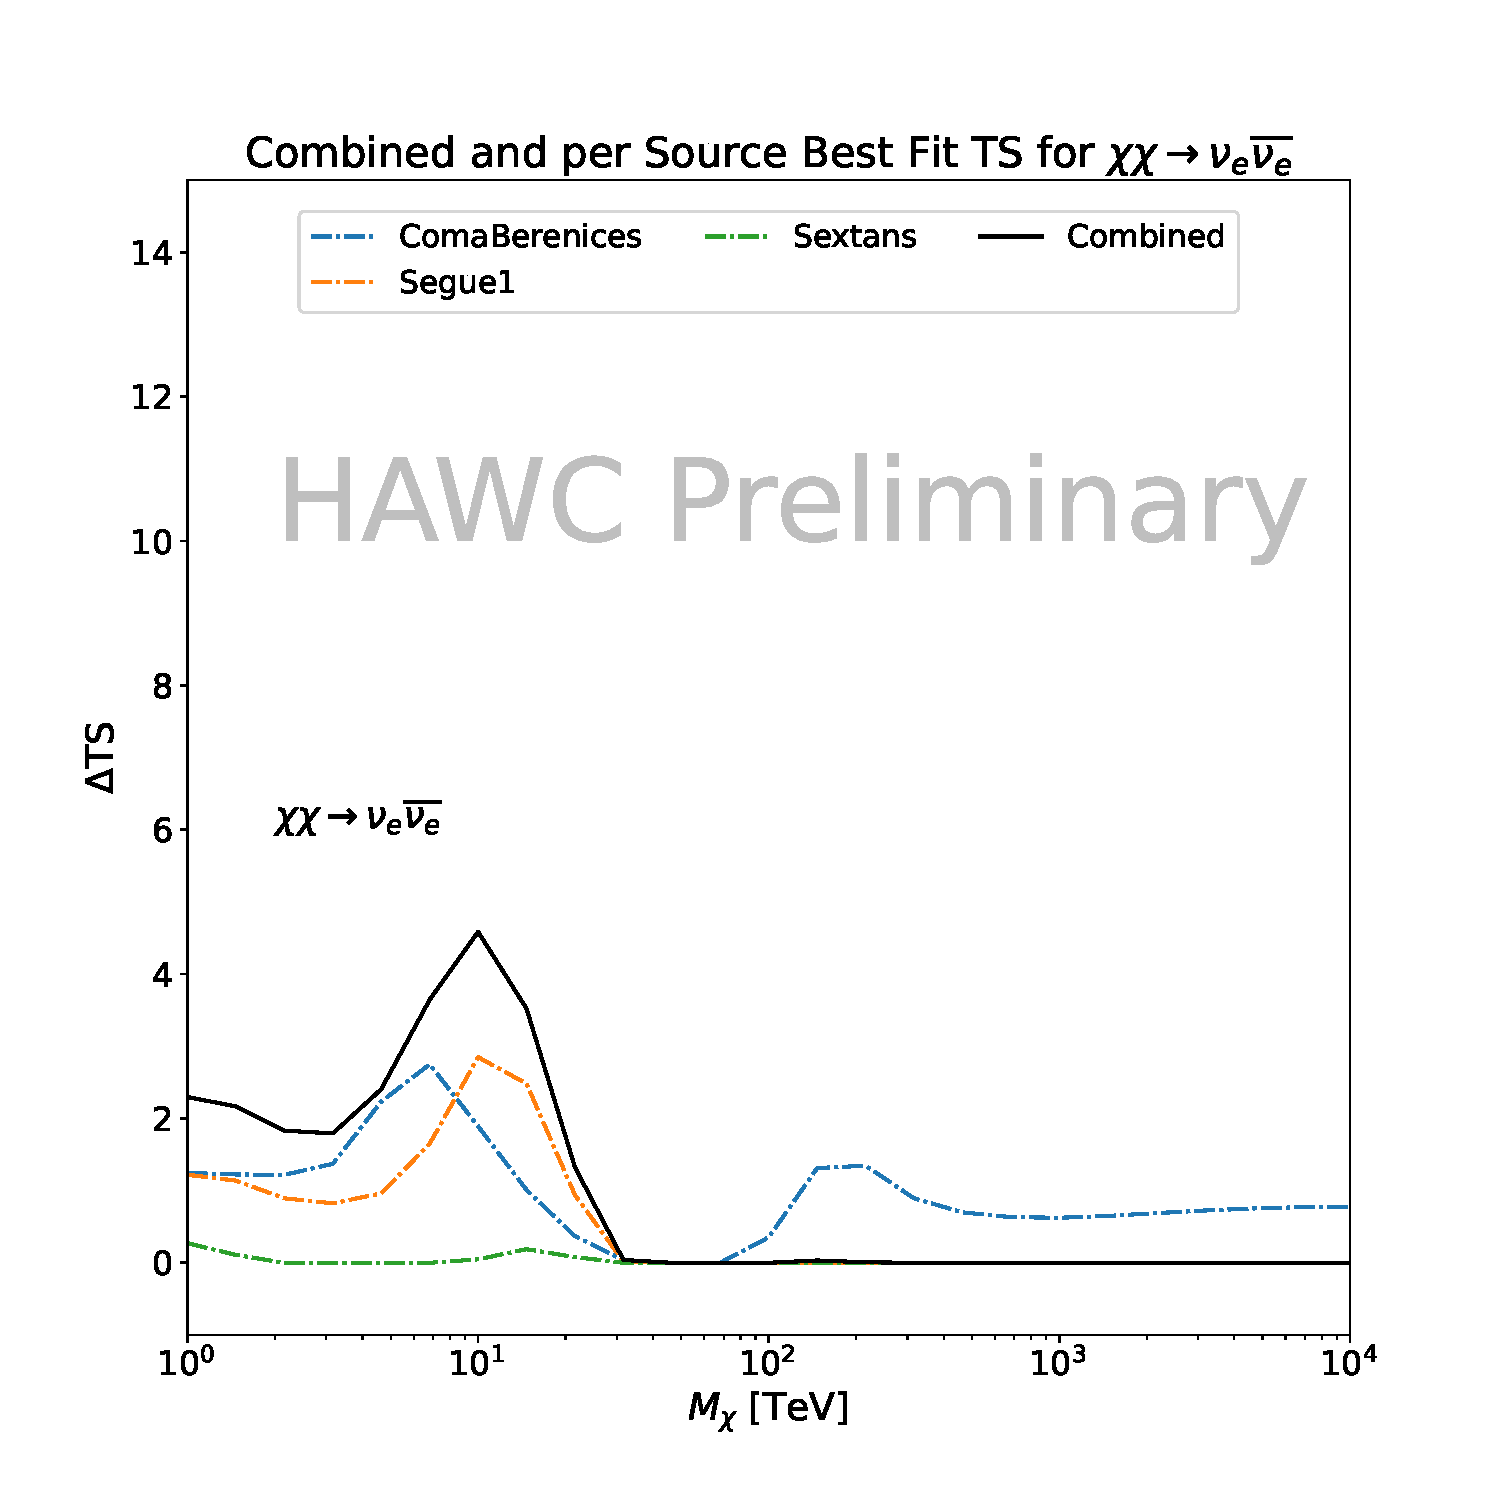
\includegraphics[scale=0.21]{figures/mtd_hawc_dm/results/CombinedTS_New_duck_nuenue_.pdf}
    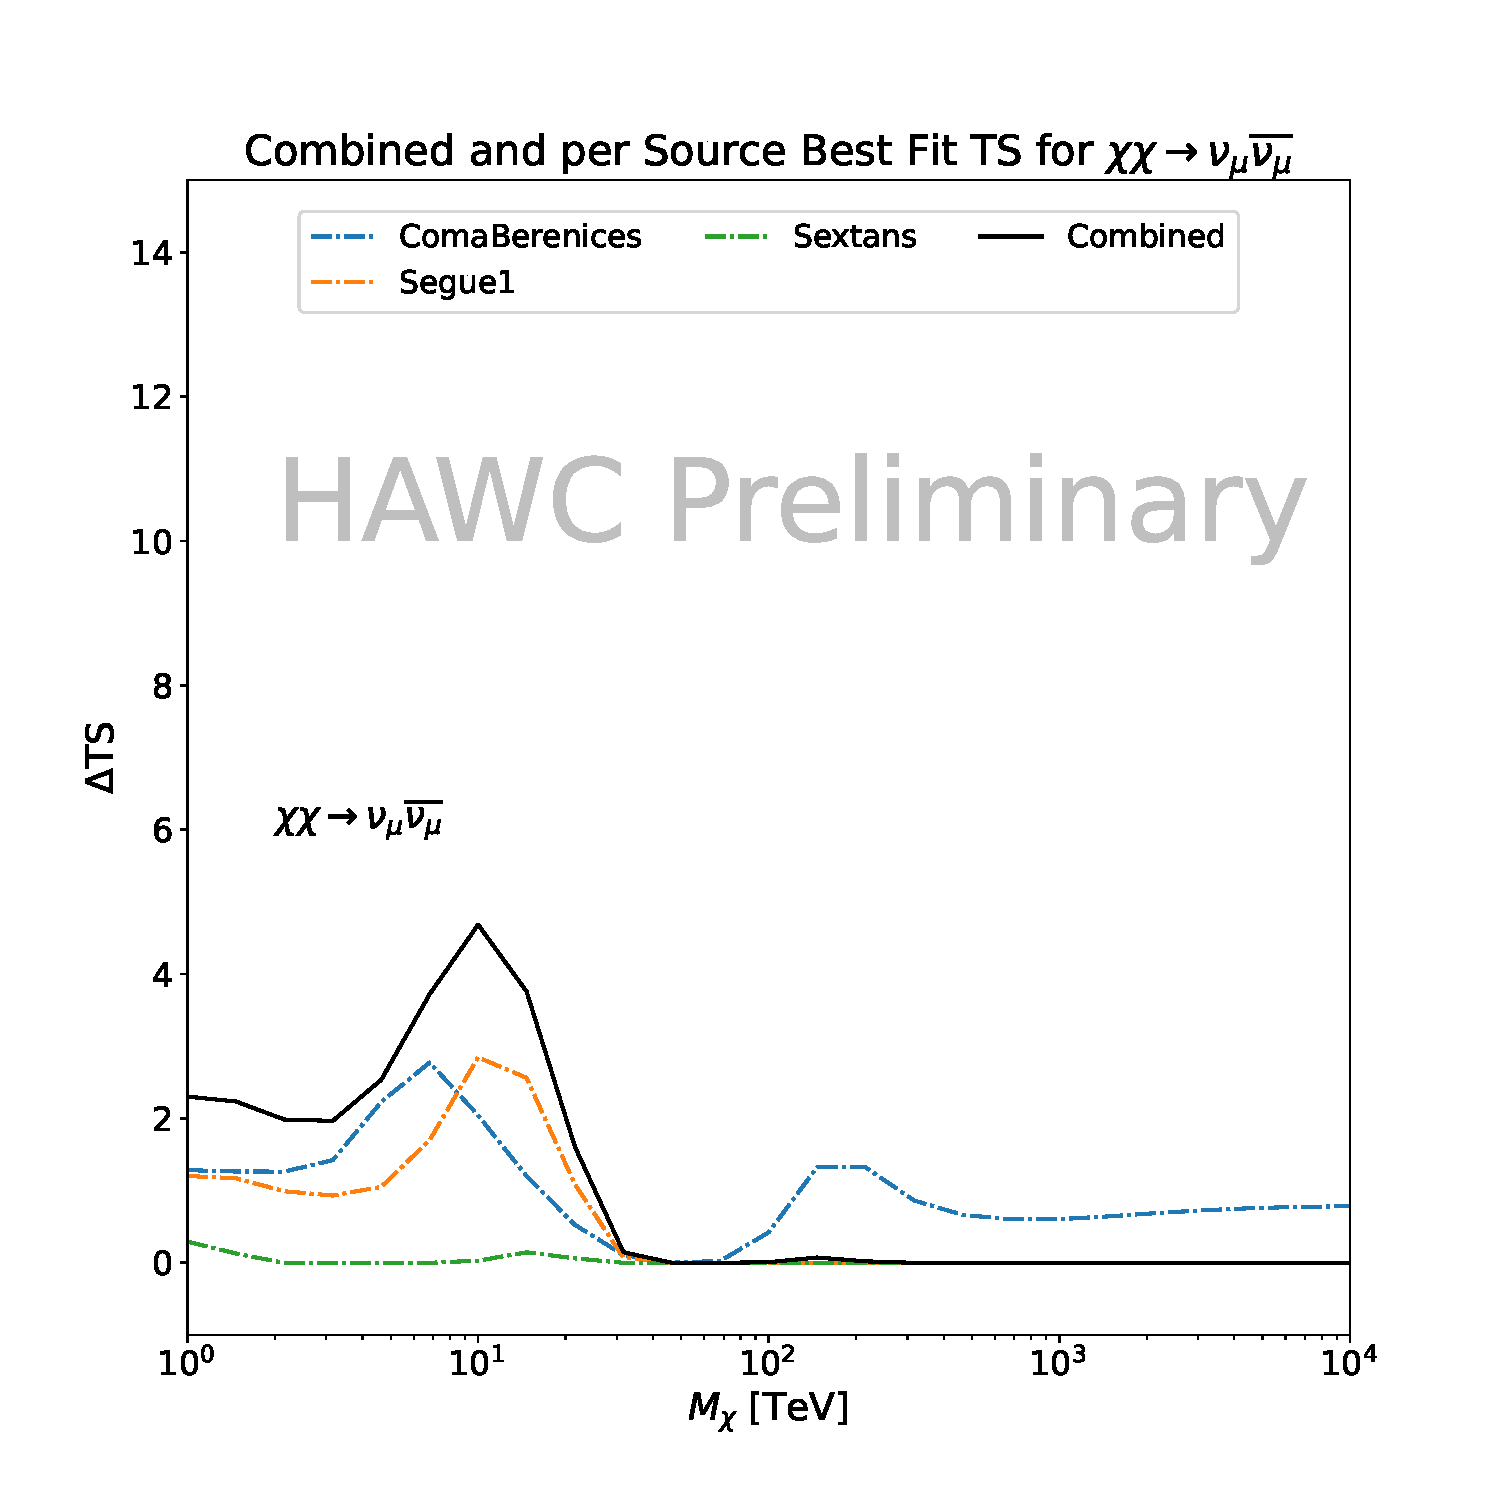
\includegraphics[scale=0.21]{figures/mtd_hawc_dm/results/CombinedTS_New_duck_numunumu_.pdf}
    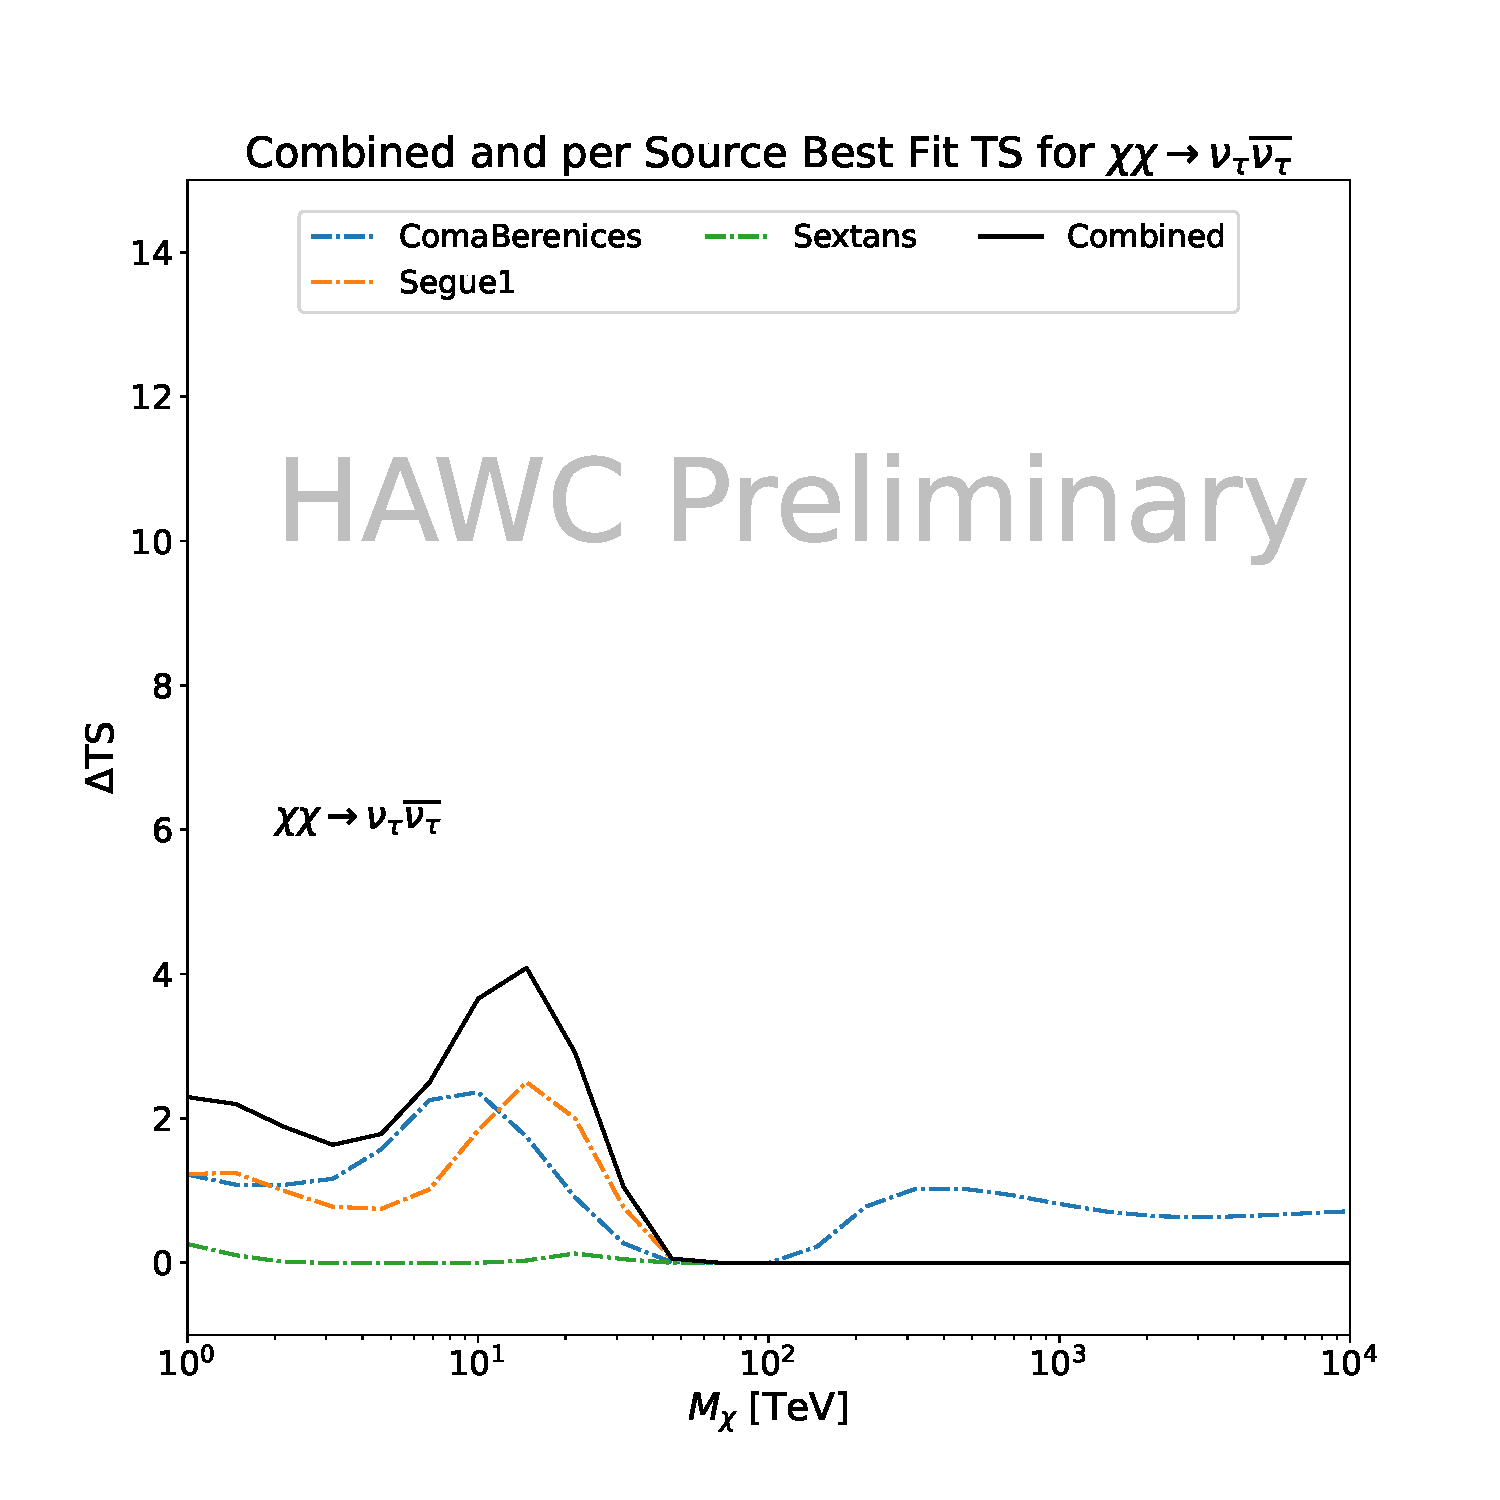
\includegraphics[scale=0.21]{figures/mtd_hawc_dm/results/CombinedTS_New_duck_nutaunutau_.pdf}
    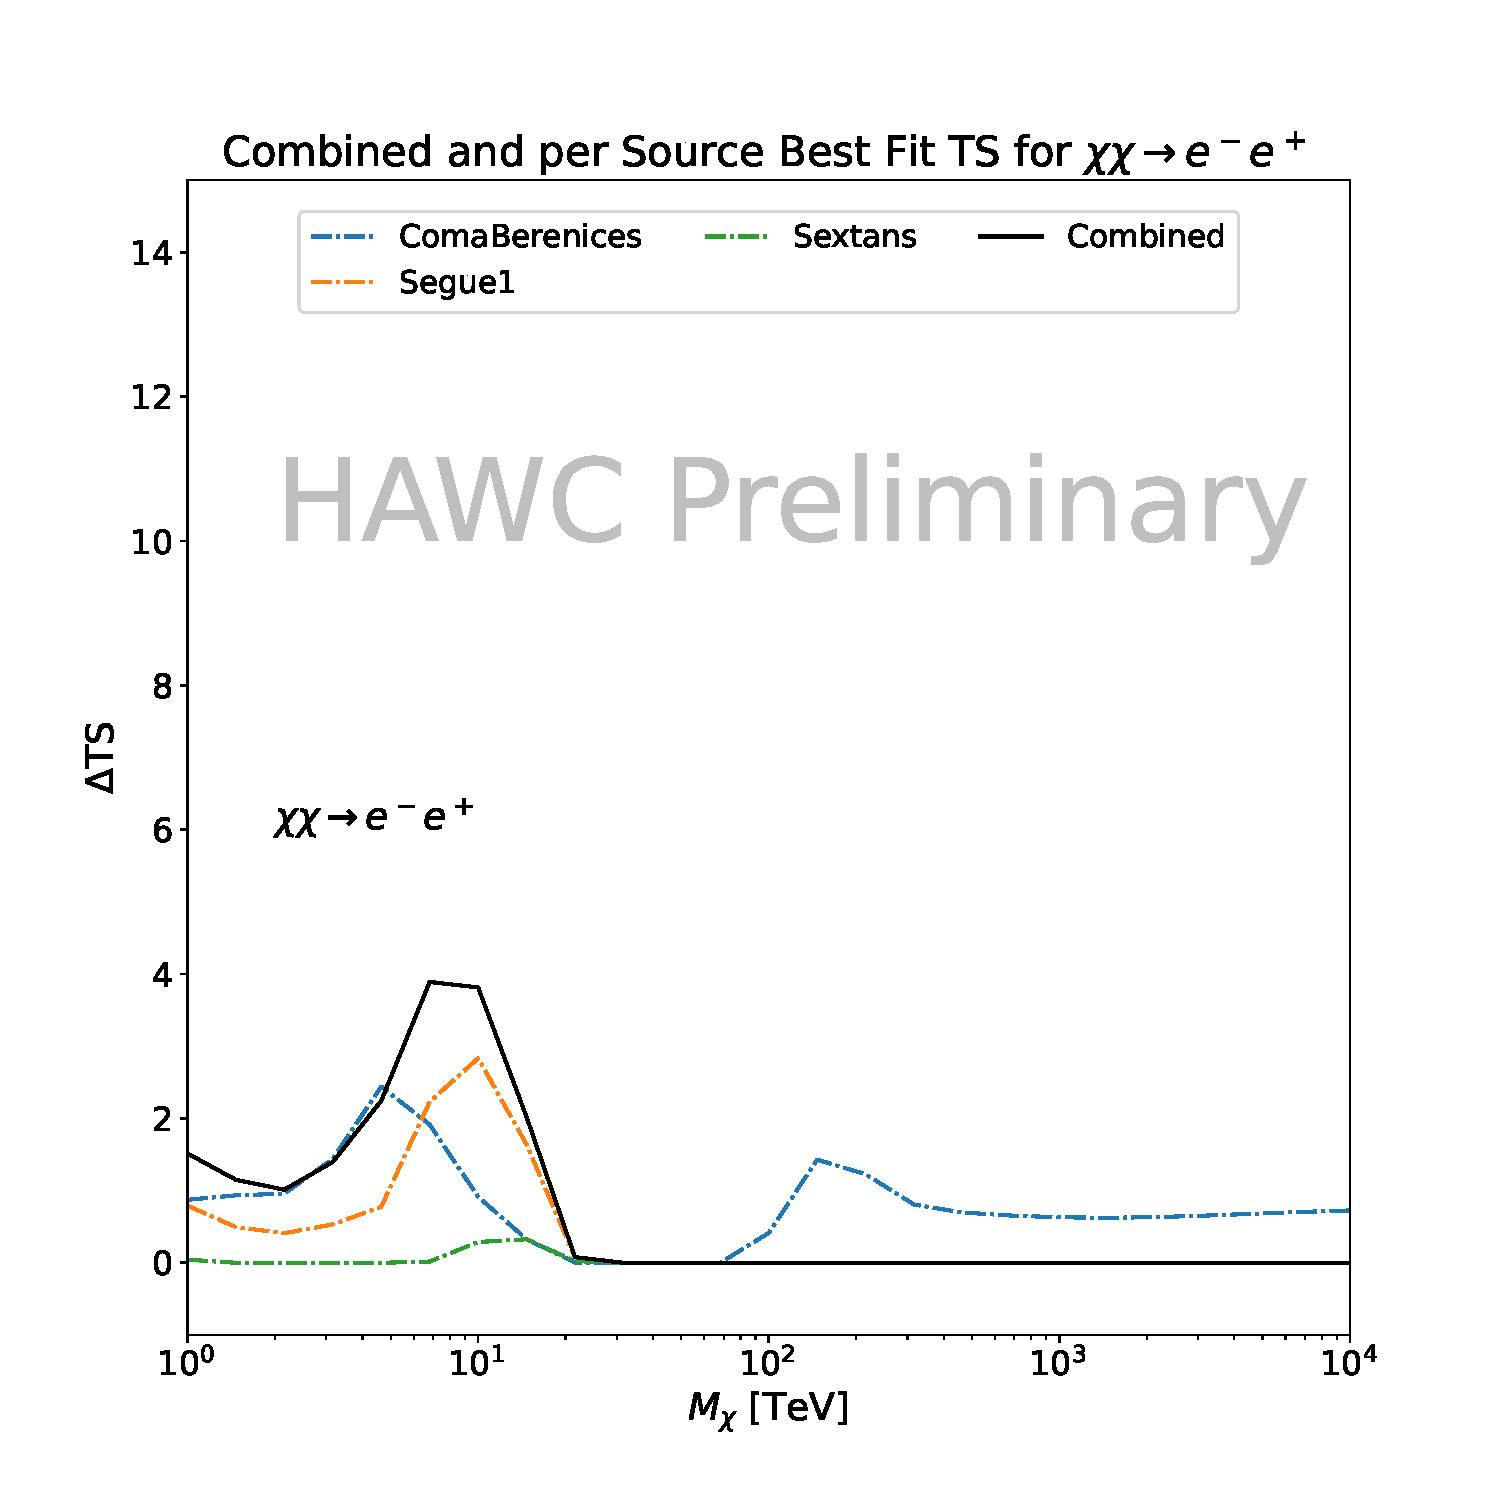
\includegraphics[scale=0.21]{figures/mtd_hawc_dm/results/CombinedTS_New_duck_ee_.pdf}
    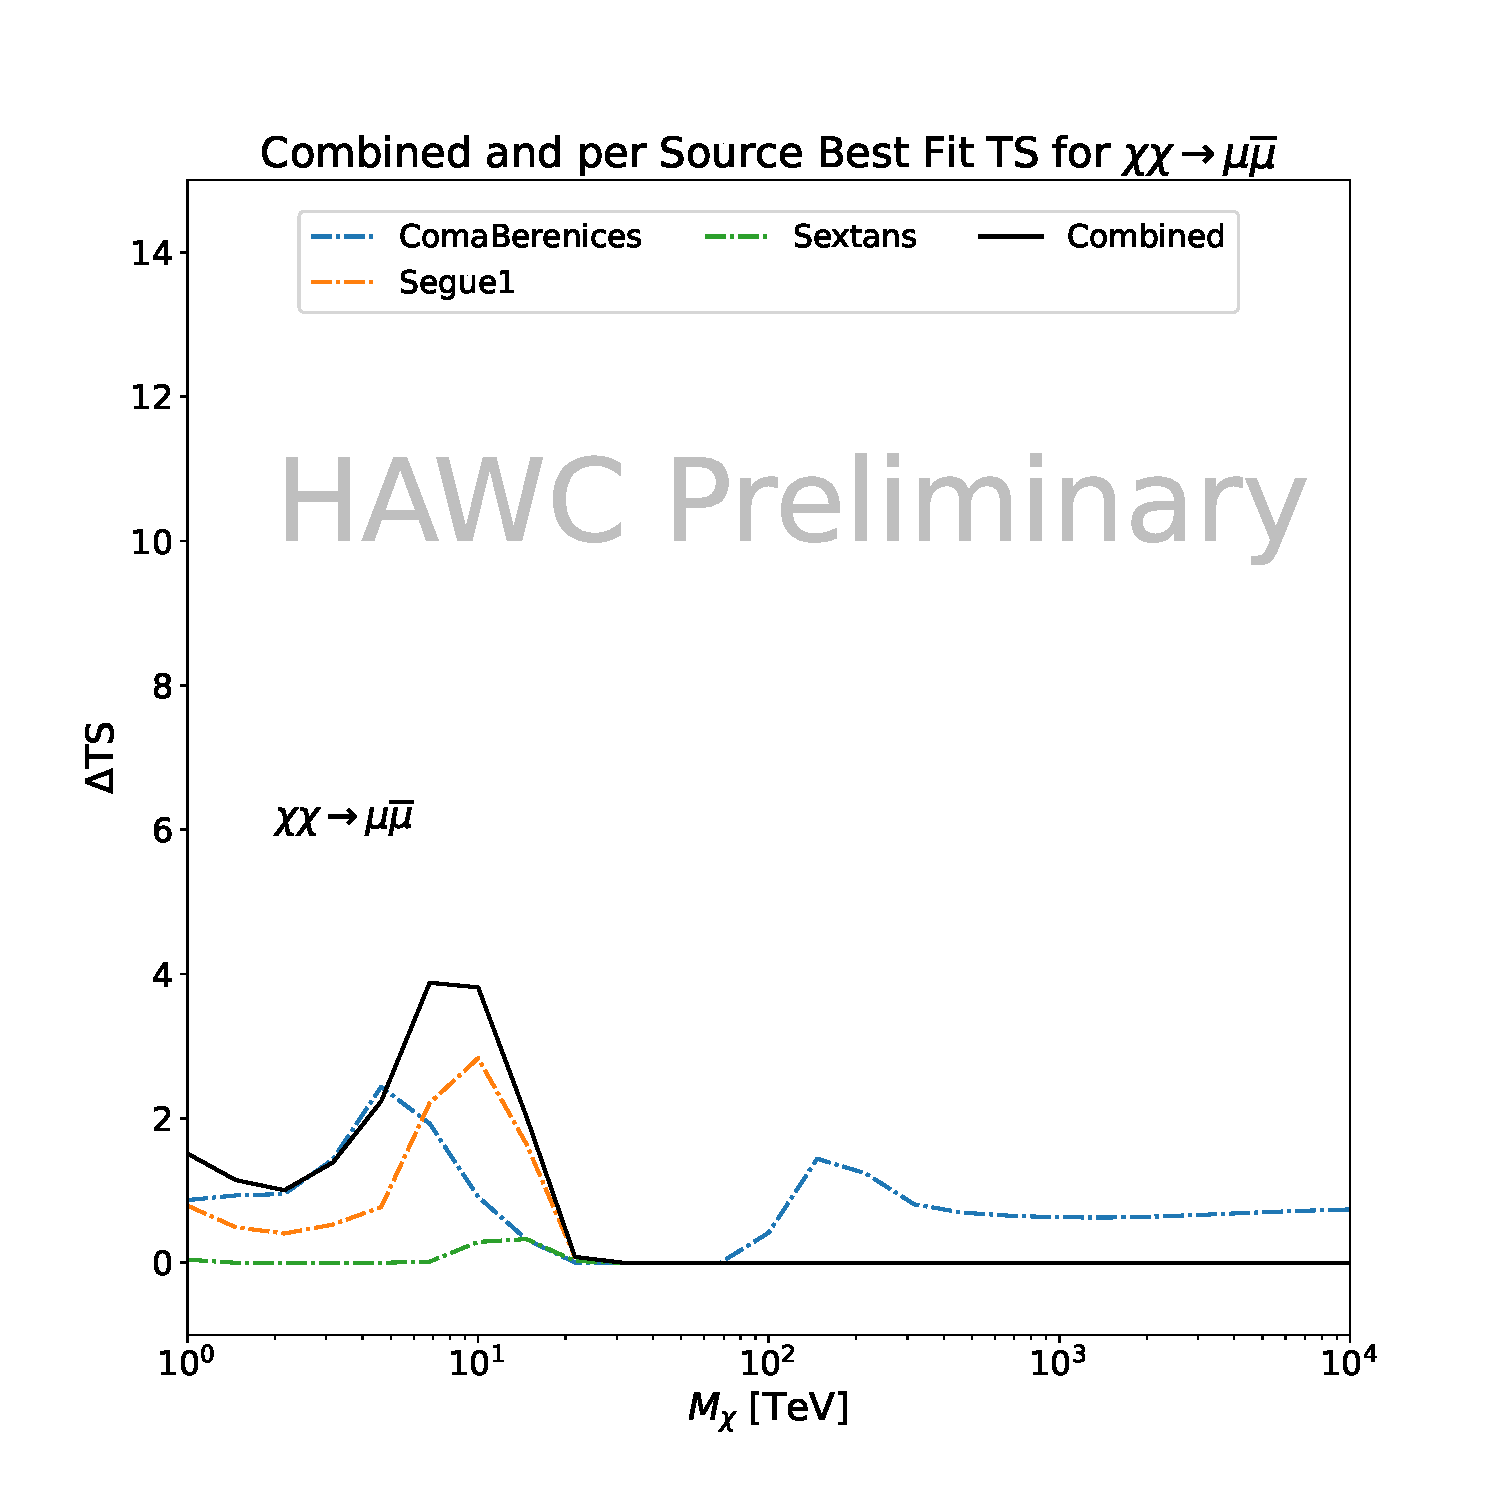
\includegraphics[scale=0.21]{figures/mtd_hawc_dm/results/CombinedTS_New_duck_mumu_.pdf}
    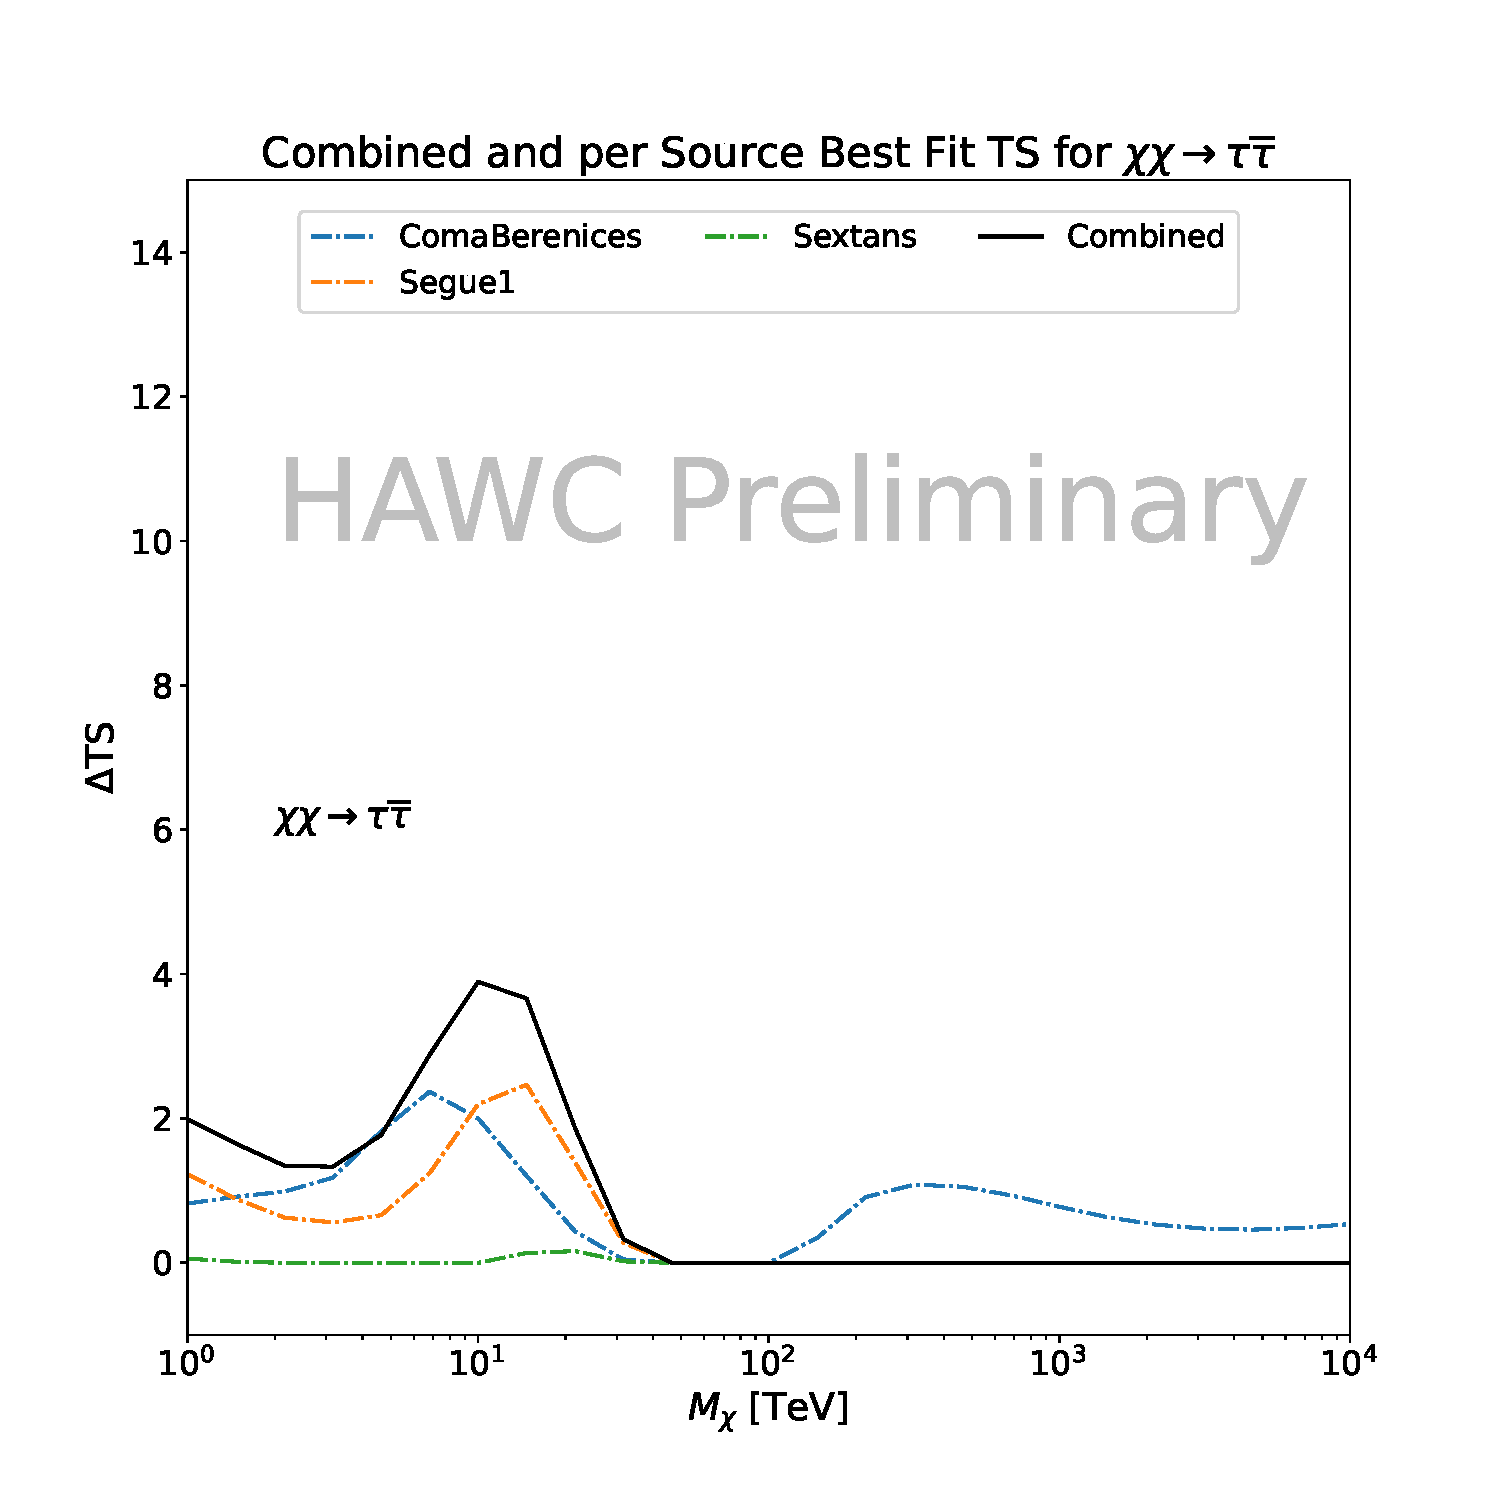
\includegraphics[scale=0.21]{figures/mtd_hawc_dm/results/CombinedTS_New_duck_tautau_.pdf}
    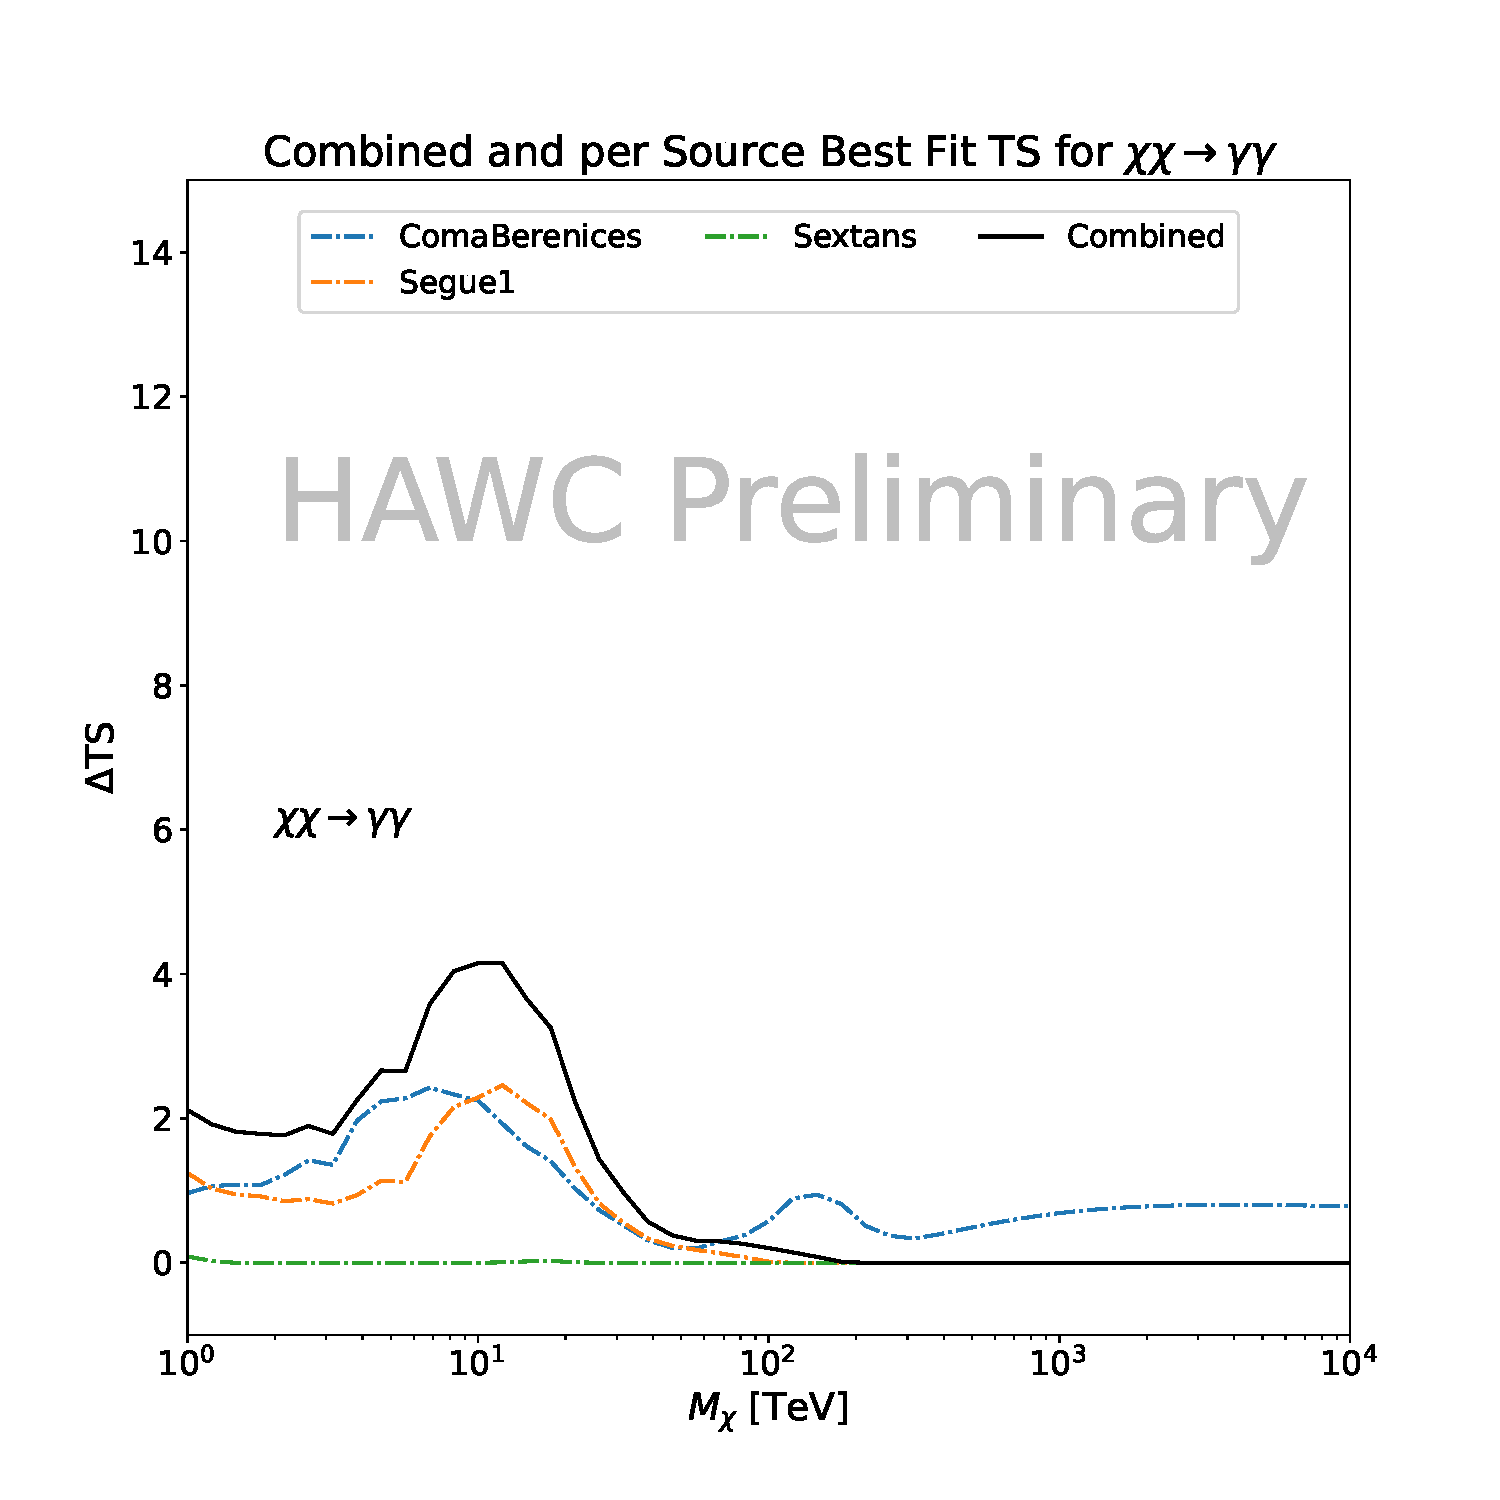
\includegraphics[scale=0.21]{figures/mtd_hawc_dm/results/CombinedTS_New_duck_gammagamma_.pdf}
    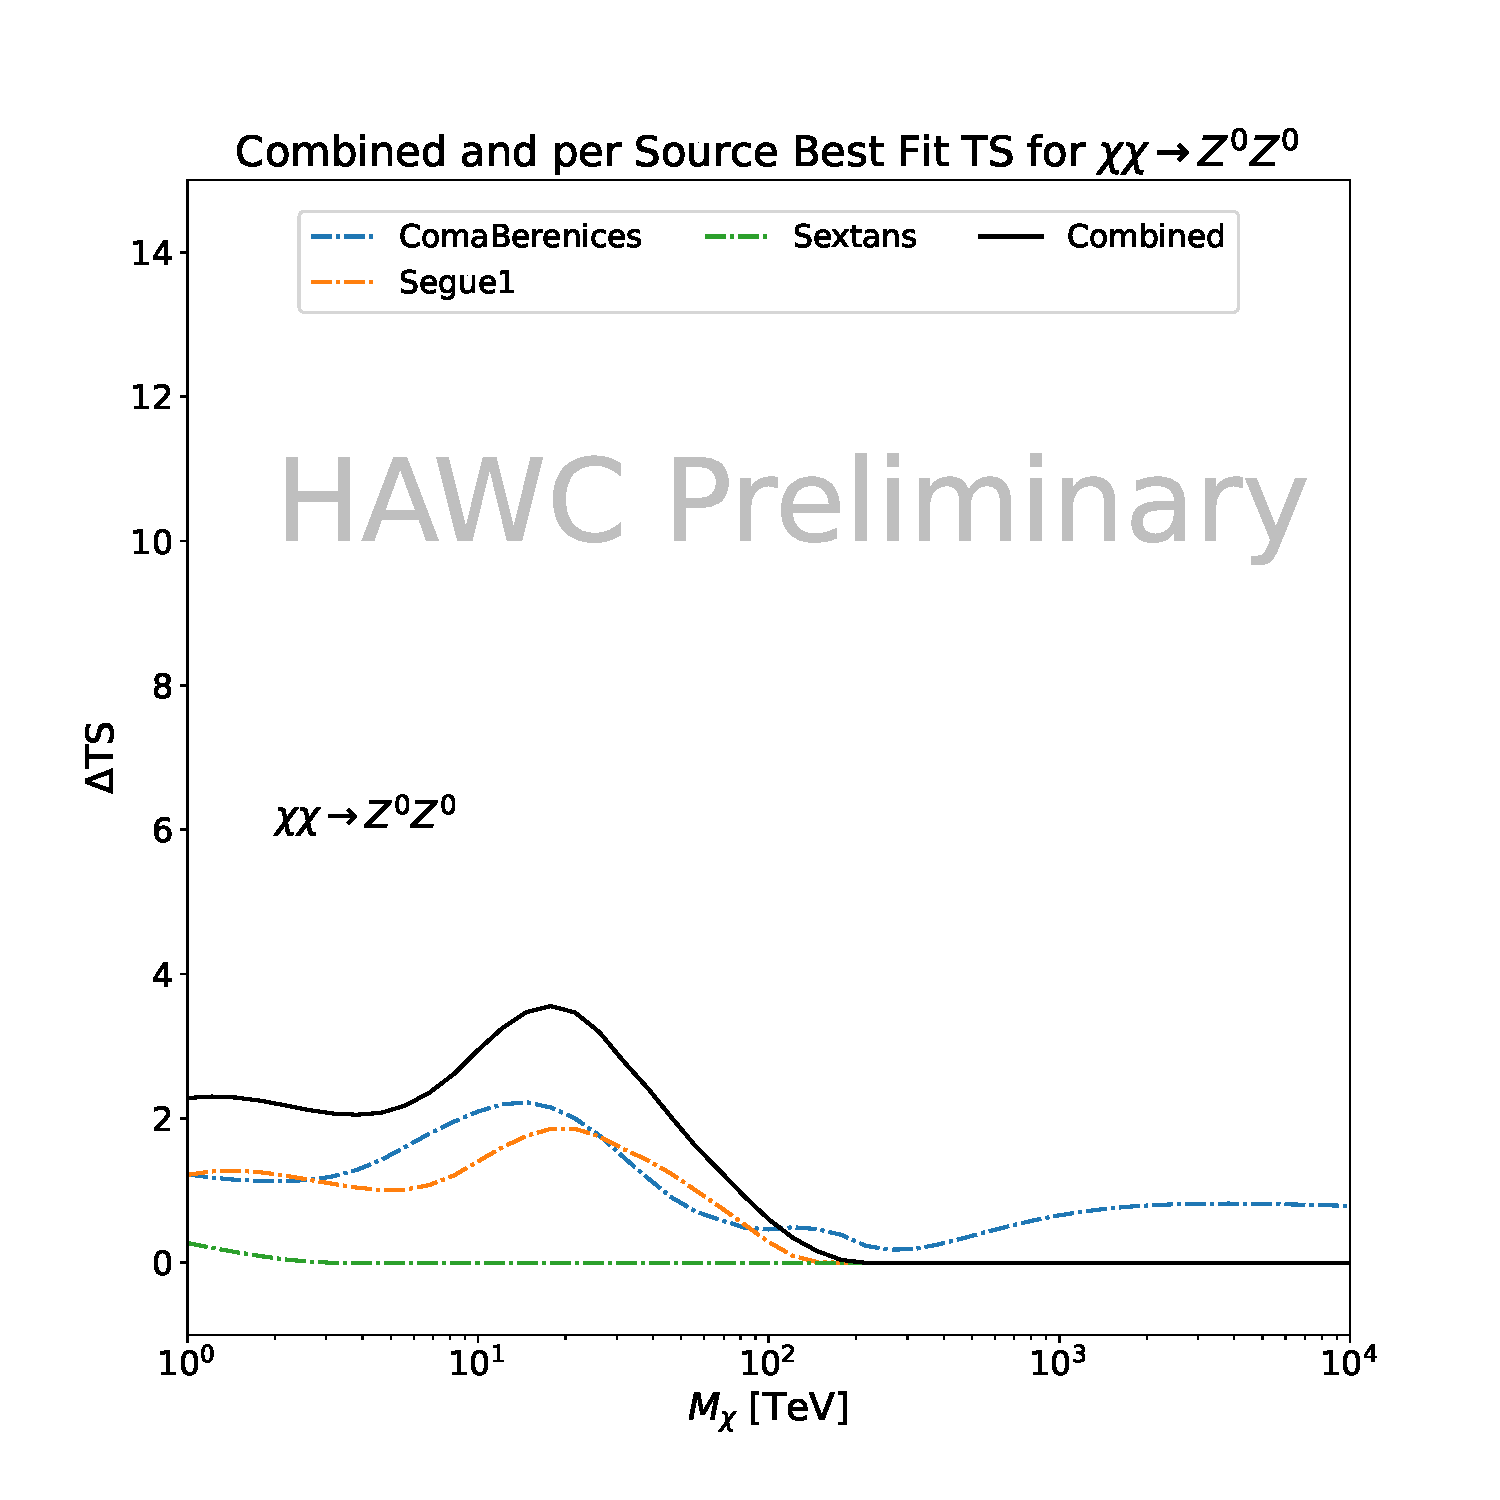
\includegraphics[scale=0.21]{figures/mtd_hawc_dm/results/CombinedTS_New_duck_zz_.pdf}
    }
    \caption{HAWC TS values for best fit \sv~versus $m_\chi$ for SM annihilation channels: $\chi\chi \rightarrow $ \parpar{\nu_e}, \parpar{\nu_\mu}, \parpar{\nu_\tau}, \parpar{e}, \parpar{\mu}, \parpar{\tau}, \pp{\gamma} and \pp{Z}. Limits use \LS \J-factors. The solid black line shows the combined best fit TS values. The colored, dashed lines are the TS values from each dSph.}
\label{fig:mtd_TS_2of2}
\end{figure}

No DM was found in HAWC observations.
The largest excess found in HAWC data was for DM annihilating to $W$-bosons or \parpar{\nu_e} for $m_\chi = 10$~TeV at significance $2.11\sigma$ and $2.14\sigma$ respectively.
HAWC's limits and excesses are dominated by Segue1.
Coma Berenices shows excesses at higher DM mass, yet no similar excesses were observed in Segue1 or Sextans.
Sextans did not contribute significantly to signal excesses or the combined limit as it is at high zenith.
Draco is at a high zenith for HAWC, so the effort required to include it was not justified by the benefits.

\begin{figure}[h]
\centering{
    \begin{tabular}{cccc}
        & Segue1 & Coma Berenices & Sextans \\
        \rotatebox[origin=c]{90}{$\chi\chi \rightarrow b\bar{b}$} &
        \raisebox{-.5\height}{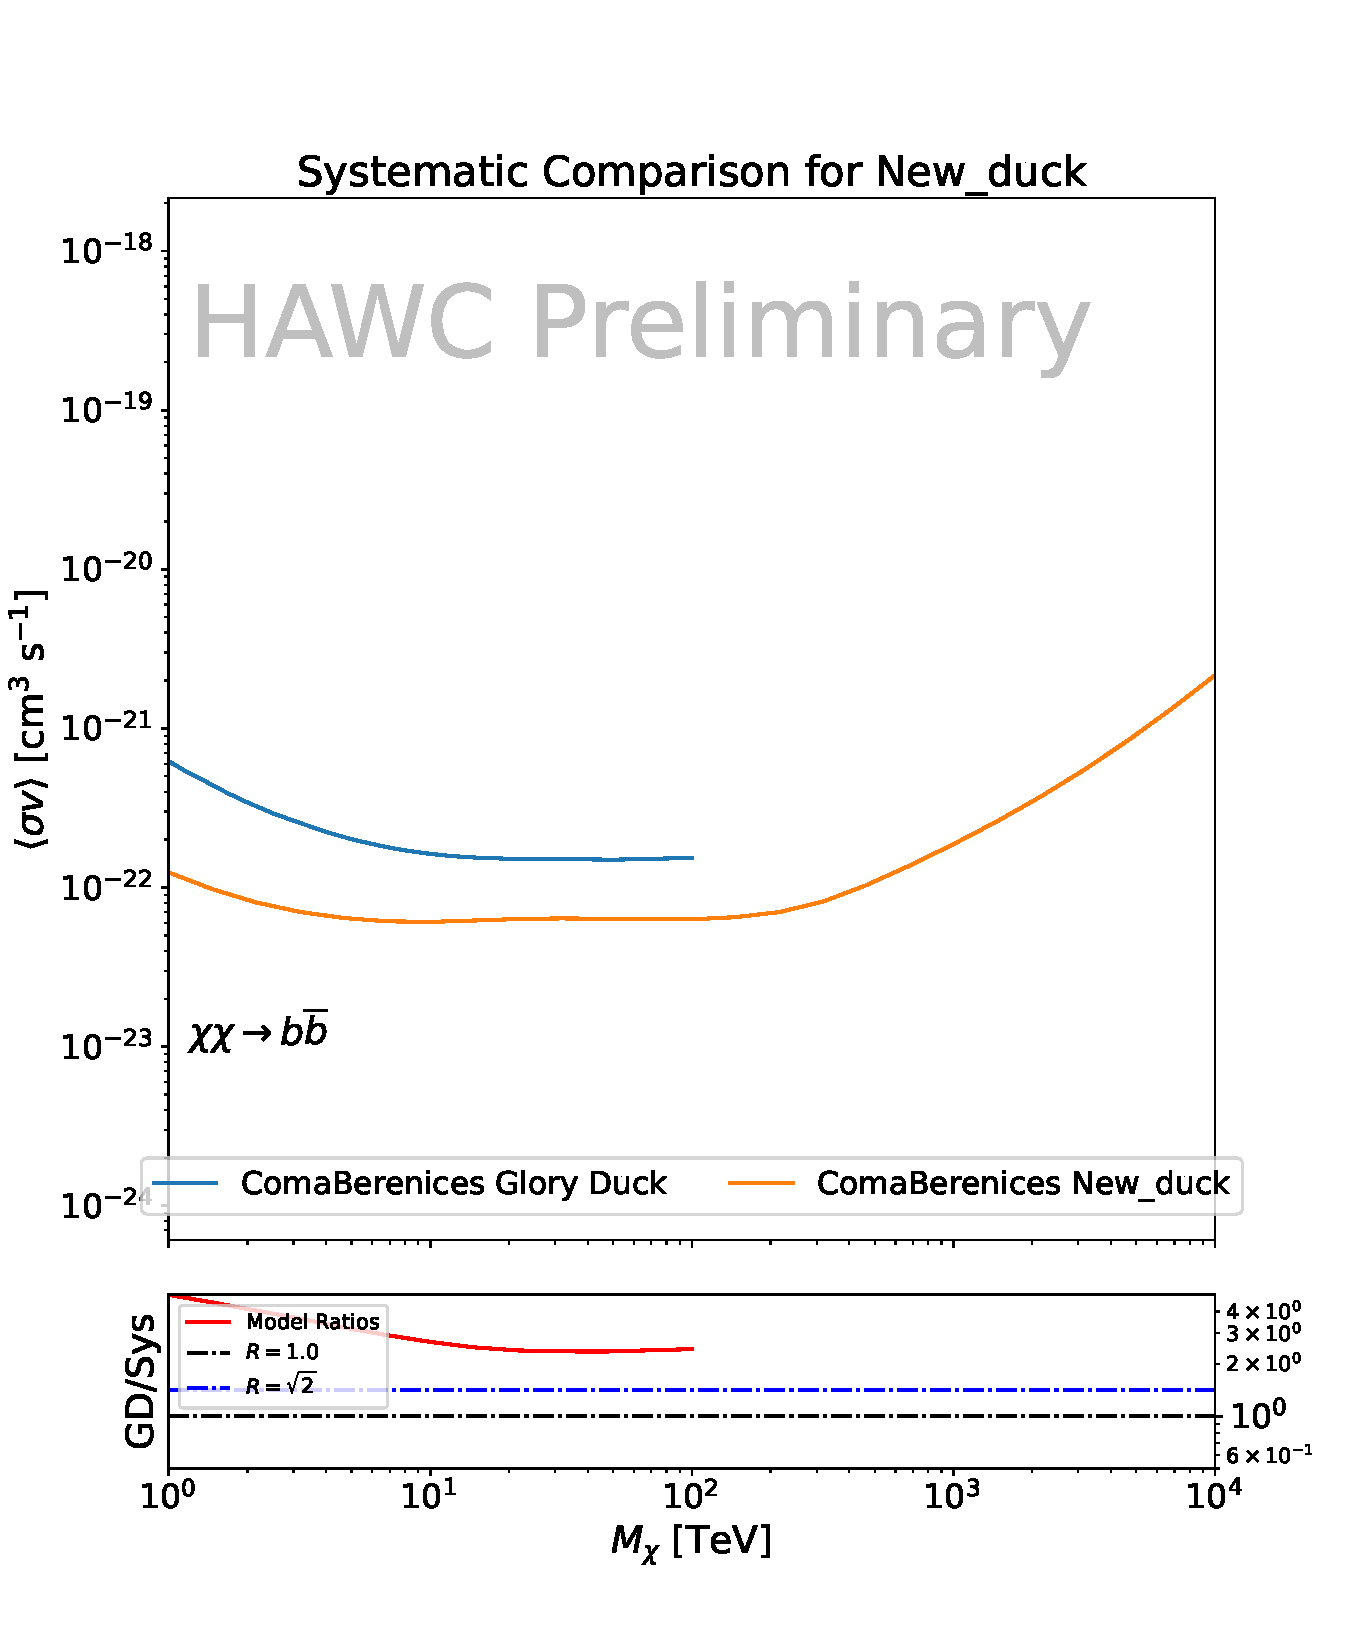
\includegraphics[scale=0.2]{figures/mtd_hawc_dm/systematics/Systematic_GD_New_duck_ComaBerenices_bb.pdf}} &
        \raisebox{-.5\height}{\includegraphics[scale=0.2]{figures/mtd_hawc_dm/systematics/Systematic_GD_New_duck_Segue1_bb.pdf}} &
        \raisebox{-.5\height}{\includegraphics[scale=0.2]{figures/mtd_hawc_dm/systematics/Systematic_GD_New_duck_Sextans_bb.pdf}} \\
        \rotatebox[origin=c]{90}{$\chi\chi \rightarrow \tau\overline{\tau}$} &
        \raisebox{-.5\height}{\includegraphics[scale=0.2]{figures/mtd_hawc_dm/systematics/Systematic_GD_New_duck_ComaBerenices_tautau.pdf}} &
        \raisebox{-.5\height}{\includegraphics[scale=0.2]{figures/mtd_hawc_dm/systematics/Systematic_GD_New_duck_Segue1_tautau.pdf}} &
        \raisebox{-.5\height}{\includegraphics[scale=0.2]{figures/mtd_hawc_dm/systematics/Systematic_GD_New_duck_Sextans_tautau.pdf}} \\
        \rotatebox[origin=c]{90}{$\chi\chi \rightarrow e^-e^+$} &
        \raisebox{-.5\height}{\includegraphics[scale=0.2]{figures/mtd_hawc_dm/systematics/Systematic_GD_New_duck_ComaBerenices_ee.pdf}} &
        \raisebox{-.5\height}{\includegraphics[scale=0.2]{figures/mtd_hawc_dm/systematics/Systematic_GD_New_duck_Segue1_ee.pdf}} &
        \raisebox{-.5\height}{\includegraphics[scale=0.2]{figures/mtd_hawc_dm/systematics/Systematic_GD_New_duck_Sextans_ee.pdf}} \\
    \end{tabular}
    }
    \caption{Comparison of HAWC limits from this analysis to Glory Duck (\cref{fig:hawc_combined_limit}) for 3 dSphs and 3 DM annihilation channels: \parpar{b}, \parpar{\tau}, and \parpar{e}. Each sector shows the 95\% confidence limit from Glory Duck (blue line) and this analysis (orange line) in the top plot. The lower plot features the ratio in log scale of Glory Duck to this analysis in a red solid line. Horizontal dashed lines are for ratios of 1.0 (black) and $\sqrt{2}$ (blue). Ratios larger than 1.0 are for limits smaller, or stricter, than Glory Duck. Ratios larger than $\sqrt{2}$ indicates limits are stricter than a simple doubling of the Glory Duck data.}
\label{fig:mtd_compare2gd}
\end{figure}

We did not generate background trials in time of writing this thesis.
These are not shown and are an immediate next step for this analysis before publication.

When comparing these results to \cref{sec:hawc_results}, we see an overall decrease in the observed confidence limits on \sv, therefore improvement to HAWC's expected sensitivity.
This improvement is generally stronger than a doubling of data, or a factor $\sqrt{2}$ decrease.
The comparison is somewhat complex and dependent on the dSph and SM annihilation channel.
\Cref{fig:mtd_compare2gd} shows the comparisons of limits calculated for this analysis and Glory Duck (\cref{sec:hawc_results}).
Segue 1 and Coma Berenices are sources at low zenith angles where improvements to HAWC's analysis come almost entirely from energy estimation.
Differences between these two are dominantly from their differences in \J-factor, half-light radii of the dSphs, and the particle physics inputs.
Substantial gains in HAWC's analysis methods (pass 5.F) were made at high zenith which is important for sources like Sextans.
The HDM particle physics model produces almost identical spectra to the PPPC for $\chi\chi \rightarrow e^-e^+$.
This channel can be used to compare limits between dSph spatial models.
Overhead sources see modest improvement to the observed limits on \sv, while high zenith sources see an order of magnitude improvement for all DM masses.
Softer SM annihilation channels see broad improvements to the limit compared to harder channels.


%%%%%%%%%%%%%%%%%%%%%%%%%%%%%%%%%%%%%%%%%%%%%%%%%%%%%%%%%%%%%
\section{Systematics}\label{sec:mtd_systemaics}
%%%%%%%%%%%%%%%%%%%%%%%%%%%%%%%%%%%%%%%%%%%%%%%%%%%%%%%%%%%%%

Systematics to this analysis are identical to what was performed earlier in Glory Duck, \cref{sec:hawc_systematic}.
We are also sensitive to the choice in spatial template, and this was explored in \cref{sec:gd_ext_limitvs_ptsrc} and \cref{sec:gd_gsVb}.

%%%%%%%%%%%%%%%%%%%%%%%%%%%%%%%%%%%%%%%%%%%%%%%%%%%%%%%%%%%%%
\section{Conclusion and Discussion}\label{sec:mtd_conclusion}
%%%%%%%%%%%%%%%%%%%%%%%%%%%%%%%%%%%%%%%%%%%%%%%%%%%%%%%%%%%%%

In this multithreaded analysis, we have used observations of 3 dSphs from HAWC to perform a collective DM annihilation search towards dSphs.
The data were combined across sources to significantly increase the sensitivity of the search.
Advanced computational techniques were deployed to accelerate wall-time spent analyzing by an order of magnitude.
We have observed no significant deviation from the null DM hypothesis, and so present our results in terms of upper limits on the velocity-weighted cross-section, \sv, for seventeen potential DM annihilation channels across four decades of DM mass.

This analysis serves as a proof of concept for multithreaded HAWC analyses with large parameter spaces.
Larger datasets with fast techniques will be essential to tackling the DM problem.
The models we used for this study include annihilation channels with neutrinos in the final state.
Advanced studies could aim to merge our results with those from neutrino observatories with large data sets.

A full HAWC analysis will include systematic studies of the \J-factor distributions.
Additionally, because of the timing reduction, the study can be doubled in size to include DM decay.
We have not yet received the remaining spatial profiles to the \LS catalog, and limits can be quickly computed once these are received.
Finally, statistical studies with Poisson variation of HAWC's background are essential to a comprehensive understanding of our observed excesses.